\chapter{Comparison across channels}\label{chap:17}
Dark matter of \SI{1}{MeV} that scatters through a heavy mediator coupled to electrons gives a kilogram of silicon 17 events a year at $\sigmae = \SI{e-37}{cm^2}$ by creating electron--hole pairs. If the mediator couples to the electrons alone, the same particle gives $7\times10^5$ events through acoustic phonons, carried by the electrons that move with the nuclei; if the mediator is a dark photon, the particle gives no events through acoustic phonons (\cref{sec:10.2}). Both rates, from electron--hole pairs and from acoustic phonons, come from one section; most of the comparisons that an experimentalist needs are spread over seven chapters. The multiphonon rate is in \cref{chap:11}, the Migdal rate in \cref{chap:12}, the phonon-assisted rate in \cref{chap:13}, magnons and superconductors in \cref{chap:14,chap:15}, and the special targets in \cref{chap:16}, each computed with the approximations its own excitation allows. A detector, however, is built for one material and one threshold, and the question that its design faces starts from the coupling instead of the excitation: for a given coupling, which excitation of which material gives the largest rate and the lowest reachable mass, and why?

The atlas of \cref{chap:9} places each excitation of a solid, and each coupling, in the section that treats it. Read along the interaction axis, the atlas answers this question at the level of the response. For each coupling it gives the channel that dominates at each mass and threshold, the few material numbers that set the rate and reach of that channel, and how firmly those numbers rank materials once the uncertainty of every input is carried through. Which experiment to build also depends on the energy per quantum, the readout and the backgrounds; the guide to next targets of \cref{sec:21.7} combines these measurement-side quantities with the rankings of this chapter (\cref{fig:17-map}).

\begin{figure}[tbp]
  \centering
  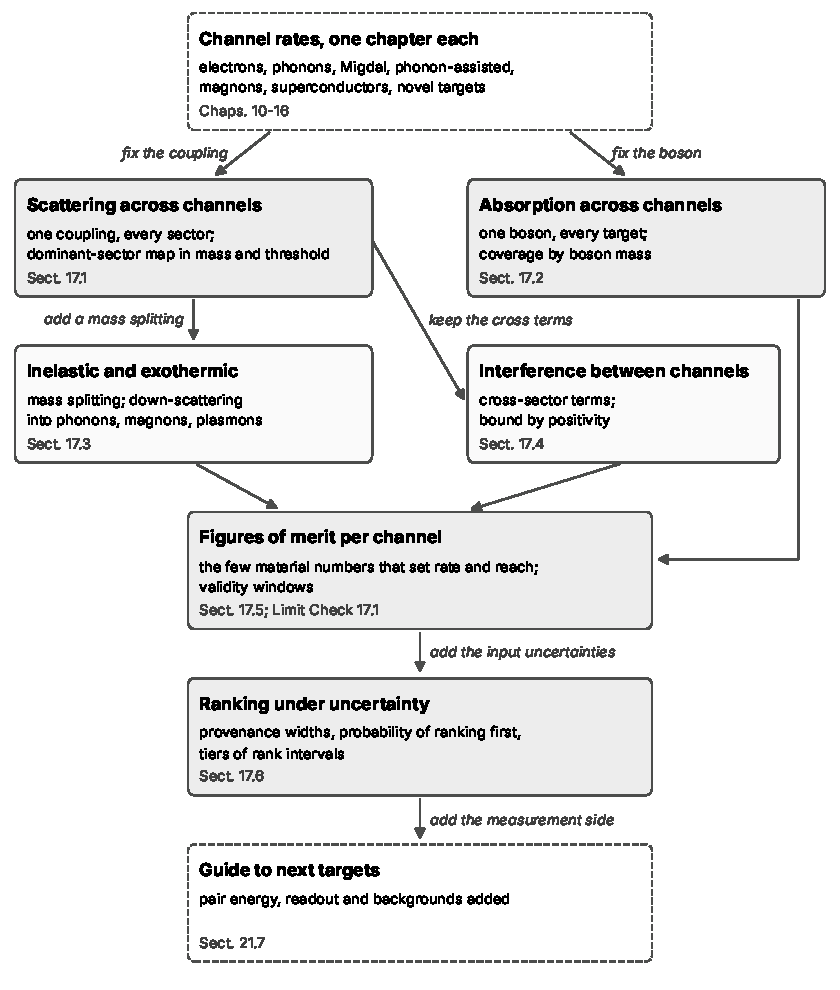
\includegraphics[width=0.85\linewidth]{figures/ch17/map17.pdf}
  \caption{Comparison across channels, from the rates of \cref{chap:10,chap:11,chap:12,chap:13,chap:14,chap:15,chap:16}. At fixed coupling: scattering in every sector and its dominant-sector map (\cref{sec:17.1}); at fixed boson: absorption on every target (\cref{sec:17.2}). Side branches: dark matter with a mass splitting, including down-scattering into collective modes (\cref{sec:17.3}), and the interference between sectors with its positivity bound (\cref{sec:17.4}). All four sections feed the figures of merit of each channel, with their validity windows (\cref{sec:17.5}; \cref{lim:17.5a}), and the ranking under the uncertainty of the inputs (\cref{sec:17.6}); the guide to next targets of \cref{sec:21.7} combines that ranking with the measurement side.}
  \label{fig:17-map}
\end{figure}

\section{Scattering across channels}\label{sec:17.1}

A silicon calorimeter with a threshold of \SI{0.1}{eV} records $3\times10^4$ events per kilogram and year from dark matter of \SI{10}{MeV} that couples to nucleons through a heavy mediator with $\sigma_p = \SI{e-38}{cm^2}$, nearly all of them multiphonon excitations of the lattice. At a threshold of \SI{0.5}{eV} it records 1.5 events, and every one of them is a Migdal ionization. Between the two thresholds the dominant final state moves from the electron-following sector of the decomposition theorem to the two electronic sectors (\cref{sec:8.6}), and the rate drops by four orders of magnitude. For each coupling, the choice of target and threshold depends on where in mass and threshold the dominant sector changes.

\subsection{Kinematic ceilings of the sectors}\label{sec:17.1-ceilings}

At fixed coupling the rate is \cref{eq:8.2-spectrum} with one coupling matrix $\mathfrak{D}$, and by the decomposition theorem \cref{eq:8.6-decomp} the structure factor is the sum of the electron-following, zero-phonon and phonon-dressed sectors. The interference between electrons and nuclei, the bottom row of \cref{tab:8-sectors}, vanishes for a coupling to one species alone (\cref{sec:17.4}). We compare two single-species couplings: a nucleon coupling, with equal couplings to protons and neutrons and the cross-section $\sigma_p$ per nucleon of \cref{sec:11.1}, and an electron coupling with the reference cross-section $\sigmae$. Both couplings have a heavy mediator. The threshold $\omega_{\mathrm{th}}$ acts on the total deposited energy, as in a calorimeter. A charge readout records the electronic sectors alone; the fraction of a lattice deposit that a phonon sensor collects is a question for the chapters on readout.

The first factor that decides the dominant sector is the largest energy that each sector can absorb. A single phonon carries at most the top of the phonon band, \SI{64.1}{meV} in silicon (\cref{sec:5.2}); the PBE density of states used for the maps ends at $\omega_{\mathrm{max}} = \SI{63.7}{meV}$ (\cref{sec:11.3}). A nucleus recoiling freely absorbs at most $E_R^{\mathrm{max}} = 2\mu_{\chi N}^2v_{\mathrm{max}}^2/M$ (\cref{eq:1.3-ERmax}), which is \SI{0.054}{eV} at \SI{10}{MeV} and \SI{5.3}{eV} at \SI{100}{MeV}. An electronic excitation can absorb up to the whole kinetic energy, $\tfrac12\mchi v_{\mathrm{max}}^2$ (\cref{eq:1.3-omegamax}), since the lattice can take the momentum without taking the energy; $\tfrac12\mchi v_{\mathrm{max}}^2$ is \SI{3.5}{eV} at \SI{1}{MeV} and \SI{35}{eV} at \SI{10}{MeV}. For $\mchi \ll M$ the electronic ceiling exceeds $E_R^{\mathrm{max}}$ by the factor $M/4\mchi$, $6.5\times10^3$ at \SI{1}{MeV}. Below the lattice ceiling the electron-following sector dominates whenever the coupling reaches the nuclei, because an electronic excitation costs a small probability per kick. Above it the electronic sectors alone are open. The boundary between the lattice and the electronic regions does not lie exactly at the lattice ceiling, however: a multiphonon spectrum extends above $E_R$ by its Poisson weights, and an impulse peak by its width.

The second factor is screening. A coupling to electrons reaches the lattice through the electrons that move with the nuclei, in full or not at all, according to whether the mediator couples to the electrons alone or to the total charge (\cref{sec:8.4}).

\subsection{Nucleon coupling in silicon}\label{sec:17.1-nucleon}

The nucleon-coupling map uses four responses. Below the zone boundary, $q \le q_{\mathrm{BZ}} = \SI{2.25}{keV}$, the one-phonon response is the long-wavelength acoustic form \cref{eq:11.1-Sac}, with the sound speeds and polarizations of the measured elastic tensor. Since the linear acoustic branches would run above every real phonon near $q_{\mathrm{BZ}}$, we cap the one-phonon deposits at $\omega_{\mathrm{max}}$. Above $q_{\mathrm{BZ}}$ the lattice response is the incoherent harmonic response \cref{eq:11.3-inc}, evaluated with the phonon density of states computed in \cref{sec:5.2} and the Helm form factor of \cref{sec:2.2}, and split into its one-phonon term and the terms with two or more phonons. Above $q = \SI{300}{keV}$, where $2W = 56$, the response is the impulse Gaussian \cref{eq:11.4-IAgauss}. The Migdal rate uses the soft-limit probability \cref{eq:12.3-soft}, evaluated with the loss function with local fields and with the $Z_{\mathrm{ion}}(p)$ of \cref{sec:12.3}. Since the sum rule \cref{eq:12.4-harm} holds at every momentum transfer in its incoherent form (for momentum transfers below $2q_{\mathrm{BZ}}$, see the qualifier on the Migdal band later in this section and \cref{tab:17-nuisances}), the lattice only has to conserve energy, and we give the lattice its mean share of the deposit, $q^2/2M$, so that the deposited energy is $\omega_e + q^2/2M$. The share of Migdal events that leave the lattice in its initial state is $\langle\ee^{-2W(|\vect{q}-\vect{p}|)}\rangle$, averaged, with the weight of \cref{sec:12.4}, over the momentum $\vect{p}$ that the electrons take. We label a point of the map ``one phonon'' when the one-phonon rate above threshold exceeds the rate with two or more phonons. Any other point where the lattice dominates is labeled ``free recoil'' when the median momentum transfer of the lattice rate lies above the impulse onset, \SI{92.5}{keV} (\cref{sec:11.4}). The electron rates are counted from \SI{1.11}{eV}, the gap in the step model of pair creation that is distributed with the loss-function tables. The tables themselves are scissored to the measured gap of \SI{1.17}{eV} (\cref{sec:10.10}), and counting from \SI{1.11}{eV} instead of \SI{1.17}{eV} moves the onset of the electron sector from 0.333 down to \SI{0.316}{MeV}.

\begin{figure}[tbp]
  \centering
  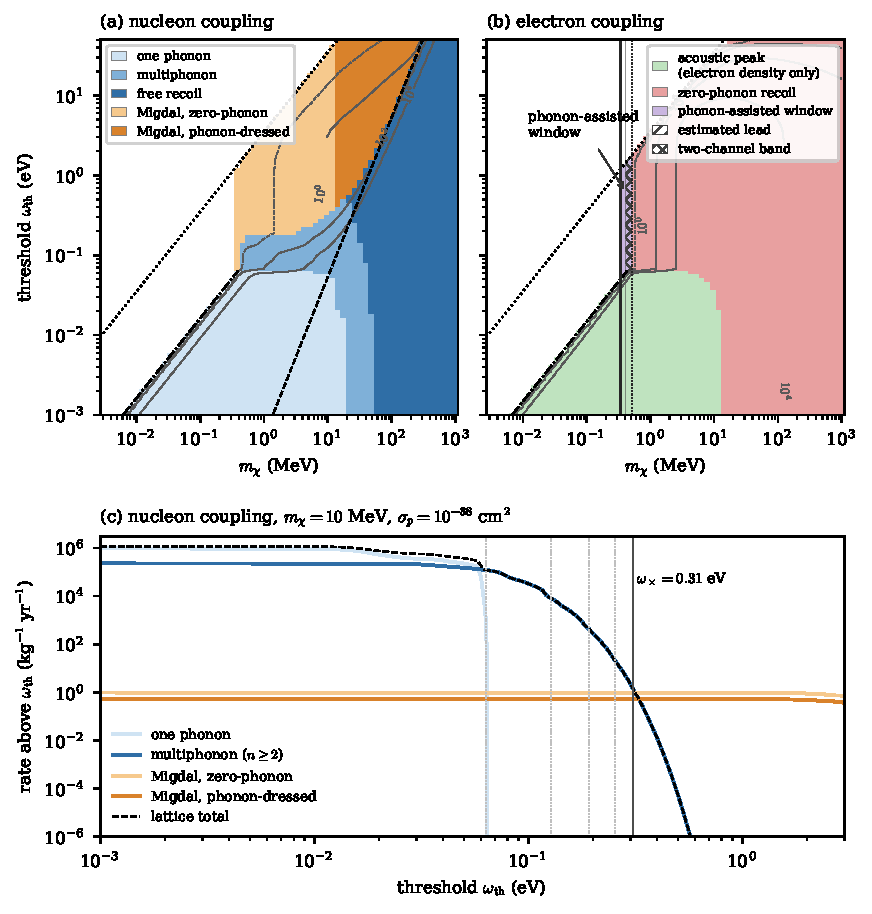
\includegraphics[width=0.86\linewidth]{figures/ch17/fig17_sectors.pdf}
  \caption{Dominant sector of silicon in the plane of dark-matter mass and threshold on the total deposited energy, heavy mediator, standard halo (\cref{tab:1-shm}), $T = 0$. (a)~Nucleon coupling: electron-following sector split into one phonon, two or more phonons and free recoil; Migdal effect split by whether more than half of the events leave the lattice in its initial state; below about \SI{2}{MeV} the Migdal rate carries the unsized coherent factor of \cref{tab:17-nuisances} (at \SI{3}{MeV} the factor acts on \SI{7}{\percent} of the Migdal rate). One-phonon deposits are capped at the top of the PBE band, \SI{63.7}{meV}. Gray contours: the dominant rate, $10^{-2}$ to $10^4$ events per kilogram and year at $\sigma_p = \SI{e-38}{cm^2}$. (b)~Electron coupling: zero-phonon electron recoil (loss function with local fields, counted from \SI{1.11}{eV}) against the acoustic peak of an electron-only coupling (absent for a dark photon) in the model of \cref{lim:10.2a} (linear longitudinal branch to $|\vect{q}| = 2\pi/a$, 28 electrons per cell following the nuclei). Phonon-assisted window from \cref{tab:13-window}: onsets 0.3332 (dashed) and \SI{0.3374}{MeV} (solid) and first zero-phonon edge 0.405--\SI{0.408}{MeV} (dark band), computed; estimated phonon-assisted lead to \SI{0.43}{MeV} (hatched) and two-channel band 0.43--\SI{0.51}{MeV} (cross-hatched). Contours at $\sigmae = \SI{e-37}{cm^2}$. Lines: dotted, the largest deposit $\tfrac12\mchi v_{\mathrm{max}}^2$; dashed, the free-recoil endpoint $E_R^{\mathrm{max}}$; dash-dotted, the acoustic edge \cref{eq:11.1-edge} with $c_{\mathrm{LA,max}} = \SI{9.35}{km/s}$ in (a) and the model's \SI{8.43}{km/s} in (b). White: no channel, or a rate below $10^{-12}$ events per kilogram and year. (c)~Rates above threshold at $\mchi = \SI{10}{MeV}$, nucleon coupling; vertical dotted lines at multiples of the band top, solid line at the crossover threshold $\omega_{\mathrm{th}}^\times$ of \cref{we:17-crossover}.}
  \label{fig:17-sectors}
\end{figure}

\Cref{fig:17-sectors}a shows the result. Below the band top the electron-following sector holds the whole map, and inside it the one-phonon term leads up to \SI{20}{MeV} at a threshold of \SI{1}{meV}, although the kicks of a \SI{10}{MeV} particle already reach $2W = 1.8$. The reason is that the incoherent response gives the one-phonon term the Poisson weight $2W\ee^{-2W}$, and the sum of all higher orders overtakes the one-phonon weight only at $2W = 1.26$. The heavy mediator weights the largest momentum transfers, so the boundary of the one-phonon region follows the typical kick. Below \SI{3.4}{MeV}, where $q_{\mathrm{max}} < \SI{18}{keV}$, the one-phonon contours carry the coherent correction of \cref{sec:11.3}, which exceeds \SI{10}{\percent} below \SI{18}{keV}; the boundary of the one-phonon region near \SI{20}{MeV}, where the kicks lie far above \SI{18}{keV}, does not. Multiphonon deposits dominate above \SI{20}{MeV} at the lowest thresholds and, at every mass, at thresholds above the band top. By the median criterion the free recoil leads above \SI{60}{MeV} at \SI{1}{meV}, and above \SI{22}{MeV} at higher thresholds. At the lowest thresholds the lattice rate exceeds the Migdal rate by roughly the inverse of the Migdal probability per kick, averaged over the kicks: by $6\times10^7$ at \SI{1}{MeV}, $8\times10^5$ at \SI{10}{MeV} and $2\times10^4$ at \SI{100}{MeV}.

\begin{table}[tbp]
  \caption{The multiphonon--Migdal crossover in silicon: nucleon coupling, heavy mediator, $\sigma_p = \SI{e-38}{cm^2}$, threshold on the total deposited energy. Largest momentum transfer and its Debye--Waller exponent; crossover threshold $\omega_{\mathrm{th}}^\times$ (lattice rate equal to the Migdal rate) and its ratio to the free-recoil endpoint; Migdal rate at the lowest thresholds (events per kilogram and year) and its zero-phonon share.}
  \label{tab:17-crossover}
  \centering\small
  \begin{tabular}{@{}lccccccc@{}}
    \toprule
    $\mchi$ (MeV) & 1 & 3 & 6.3 & 10 & 17.5 & 30 & 100 \\
    \midrule
    $q_{\mathrm{max}}$ (keV) & 5.3 & 15.9 & 33.4 & 53.0 & 92.7 & 159 & 528 \\
    $2W(q_{\mathrm{max}})$ & 0.02 & 0.16 & 0.70 & 1.76 & 5.40 & 15.9 & 175 \\
    $\omega_{\mathrm{th}}^\times$ (eV) & 0.178 & 0.187 & 0.242 & 0.307 & 0.466 & 0.826 & 5.33 \\
    $\omega_{\mathrm{th}}^\times/E_R^{\mathrm{max}}$ & 331 & 38.8 & 11.3 & 5.73 & 2.84 & 1.71 & 1.00 \\
    Migdal rate & $1.9\times10^{-3}$ & 0.12 & 0.68 & 1.5 & 3.4 & 6.9 & 30 \\
    zero-phonon share & 0.97 & 0.94 & 0.83 & 0.65 & 0.33 & 0.10 & 0.001 \\
    \bottomrule
  \end{tabular}
\end{table}

The Migdal effect holds the band between the end of the lattice spectrum and the largest deposit. The Migdal band opens at a mass of $2\Eg/v_{\mathrm{max}}^2$. Up to \SI{1}{MeV} the Migdal rate comes from momentum transfers between about \SI{0.75}{keV} and $2q_{\mathrm{BZ}}$, where the diagonal soft limit of \cref{sec:12.4} is not known to equal the coherent response and the coherent response is not computed. Near threshold the factor that takes the diagonal soft limit to the coherent response is likely a large suppression, since the exact small-$q$ spectrum lies at the plasmon, beyond the energies that are open near threshold. The Migdal band at 0.32--\SI{1}{MeV} carries this unsized coherent factor, and so does the \SI{1}{MeV} column of \cref{tab:17-crossover}, since the whole Migdal rate at \SI{1}{MeV} comes from momentum transfers between about \SI{0.75}{keV} and $2q_{\mathrm{BZ}}$ (\SI{29}{\percent} of it from below $q_{\mathrm{BZ}}$). At \SI{2}{MeV} the coherent factor acts on a third of the Migdal rate, and from \SI{3}{MeV} on, on \SI{7}{\percent} or less (\cref{tab:17-nuisances}). \Cref{tab:17-crossover} gives the crossover threshold $\omega_{\mathrm{th}}^\times$, where the lattice and the Migdal rates are equal. Below \SI{3}{MeV} the kicks are soft, $2W(q_{\mathrm{max}}) \le 0.16$, and the crossover stays near $2.8$ to $2.9\,\omega_{\mathrm{max}}$. A deposit above $2\omega_{\mathrm{max}}$ needs three phonons, and the three-phonon weight scales as $(2W)^3$, against $2W$ for the Migdal probability; the three-phonon spectrum falls so steeply at its top that a smaller $2W$ moves the crossover little. Between 3 and \SI{20}{MeV} the crossover climbs through the Poisson tail of the multiphonon spectrum, as \cref{we:17-crossover} works out at \SI{10}{MeV}. Above the impulse onset the lattice deposit is a peak at $E_R$ with a Gaussian tail, and the crossover moves onto the free-recoil endpoint. At \SI{300}{MeV} it lies at $0.98\,E_R^{\mathrm{max}}$, below the endpoint, because $\eta(\vmin)$ vanishes at the endpoint faster than the Migdal rate falls. Above \SI{410}{MeV} the endpoint passes the \SI{89}{eV} end of the tables, and the Migdal side of the map would need the core shells (\cref{sec:12.2}). Inside the Migdal band a charge readout at the single-electron level records the Migdal events with no lattice background from the dark matter itself.

The Migdal region of \cref{fig:17-sectors}a splits at one mass into a zero-phonon and a phonon-dressed part. A zero-phonon Migdal event needs the lattice to absorb the kick coherently, with probability $\ee^{-2W}$ at the momentum the nucleus keeps. The rate-weighted share of zero-phonon events falls with mass (\cref{tab:17-crossover}), and it equals the phonon-dressed share at \SI{13.2}{MeV}. This crossing lies above the \SI{6.3}{MeV} at which a kick at the largest momentum transfer gives $\ee^{-2W} = \tfrac12$ (\cref{sec:12.4}), since the halo puts most kicks below the largest one. At \SI{300}{MeV} the Migdal rate at the lowest thresholds reaches 130 events per kilogram and year.

\begin{workedexample}{The multiphonon--Migdal crossover in silicon at 10 MeV}\label{we:17-crossover}
\emph{Kinematics.} For $\mchi = \SI{10}{MeV}$ the largest momentum transfer is $q_{\mathrm{max}} = 2\mu_{\chi N}v_{\mathrm{max}} = \SI{53.0}{keV}$, and a free recoil there would take $E_R^{\mathrm{max}} = \SI{53.7}{meV}$. With the mean phonon energy $\langle\omega\rangle = \SI{40.9}{meV}$ the recoil parameter of \cref{sec:8.5} is $x_R = E_R/\langle\omega\rangle = 1.31$, below the impulse onset $x_R = 4$ (\cref{sec:11.4}). The lattice therefore takes the energy in whole phonons, with Poisson weights of mean $2W = q^2\langle u_x^2\rangle = 1.76$, where $\langle u_x^2\rangle = \SI{2.45e-3}{\angstrom^2}$ is the mean square displacement of \cref{sec:11.3}.

\emph{Migdal side.} The Migdal probability per kick is $6.07\times10^{-5}$ per eV of recoil energy (\cref{sec:12.3}), or $3.26\times10^{-6}$ at $q_{\mathrm{max}}$, all of it at $\omega_e \ge \SI{1.11}{eV}$.

\emph{Lattice side.} The incoherent spectrum at $q_{\mathrm{max}}$ is $8.1\times10^{-3}$ per eV at \SI{0.3}{eV}, where seven phonons give \SI{35}{\percent} of it, and $1.24\times10^{-4}$ per eV at \SI{0.4}{eV}, a fall by a factor 65 per \SI{0.1}{eV}. The weight above \SI{0.4}{eV} is then $1.24\times10^{-4} \times \SI{0.024}{eV} = 3.0\times10^{-6}$, equal to the Migdal probability: per kick, the crossover lies near \SI{0.4}{eV}.

\emph{Rates.} Integrated over momentum transfer and halo, the lattice rate above 0.1, 0.2, 0.3 and \SI{0.5}{eV} is $3.3\times10^4$, 283, 2.2 and $5.5\times10^{-5}$ events per kilogram and year at $\sigma_p = \SI{e-38}{cm^2}$, against a Migdal rate of 1.5 (0.98 zero-phonon, 0.53 phonon-dressed) that does not change below \SI{1.1}{eV}. The lattice and Migdal rates are equal at $\omega_{\mathrm{th}}^\times = \SI{0.307}{eV}$, or $5.7\,E_R^{\mathrm{max}}$ and $4.8\,\omega_{\mathrm{max}}$. The rate crossover lies below the per-kick value because softer kicks lose more of their tail than of their Migdal probability: the tail scales as a high power of $2W \propto q^2$, the Migdal probability as $q^2$. Near $\omega_{\mathrm{th}}^\times$ the lattice rate falls by a factor $e$ every \SI{0.020}{eV}. The coherent corrections to multiphonon spectra near their band edges are about a factor of two in the tail (\cref{sec:11.3}), and a change of that size moves $\omega_{\mathrm{th}}^\times$ by \SI{0.014}{eV}.
\end{workedexample}

\subsection{Electron coupling and screening}\label{sec:17.1-electron}

An electron coupling reaches the zero-phonon, phonon-dressed and electron-following sectors of silicon. The zero-phonon sector gives the loss-function rate \cref{eq:10.2-rate}, open above the first zero-phonon edge at 0.405 to \SI{0.408}{MeV}, and we evaluate this rate with the loss function with local fields. The phonon-dressed sector gives the phonon-assisted rate of \cref{sec:13.3}, open from 0.3332 or \SI{0.3374}{MeV}; for the window between the phonon-assisted onset and the zero-phonon edge we take \cref{tab:13-window}, where only estimates of the phonon-assisted rate exist. The electron-following sector gives the acoustic peak of \cref{sec:10.2}, carried by the electrons that move with the nuclei. We evaluate the acoustic peak in the model of \cref{lim:10.2a}: a linear longitudinal branch with $c_{\mathrm{LA}} = \SI{8.43}{km/s}$ up to $|\vect{q}| = 2\pi/a = \SI{2.28}{keV}$, where the branch reaches \SI{64}{meV}, and all 28 electrons of the cell following the nuclei.

\Cref{fig:17-sectors}b shows the map. Below \SI{0.3332}{MeV} the acoustic peak is the one open channel, and it is open up to its top at \SI{64}{meV}. Between 0.3332 and \SI{0.405}{MeV} the phonon-assisted channel is the one electronic channel; by the estimates of \cref{sec:13.9} it leads centrally to \SI{0.43}{MeV}, the phonon-assisted and zero-phonon channels are comparable from 0.43 to \SI{0.51}{MeV}, and above \SI{0.51}{MeV} the zero-phonon rate leads. Wherever the acoustic peak is open, it dominates the low thresholds: it exceeds the electron-recoil rate by $4.4\times10^4$ at \SI{1}{MeV} and by 1.2 at \SI{10}{MeV}, and the two rates are equal at \SI{12.3}{MeV}, above which the electron recoil leads at every threshold. The crossing at \SI{12.3}{MeV} is a property of the model, however. In the model the acoustic peak stops at \SI{2.28}{keV}, a momentum transfer that dark matter of \SI{0.43}{MeV} already reaches, and above that mass the peak falls as $1/(\mchi\mu_{\chi e}^2)$, while the electron recoil keeps gaining phase space at large $q$ up to \SI{10}{MeV}. Umklapp terms, the transverse branches and the multiphonon deposits of the following charge are all absent from the model and would add to the peak; the bending of the dispersion and the loss of following charge at finite $q$ would take from the peak (\cref{sec:10.2}).

Screening decides which of the low-threshold regions exists. For a coupling proportional to the total charge, as for a dark photon, the exactness theorem \cref{eq:8.4-exact} makes $S_{ZZ}$ proportional to the loss function at every $(q,\omega)$ with the nuclei free to move. The loss function of silicon has no acoustic peak at order $q^2$: the Born charges vanish, so the electrons that follow a displaced nucleus cancel its charge, and the acoustic weight of $S_{ZZ}$ starts at order $q^4$ (\cref{sec:8.4}). For a dark photon the green region of \cref{fig:17-sectors}b is empty to the order computed in this book, and silicon below \SI{0.3332}{MeV} has no channel. For a mediator that couples to the electrons alone, on the other hand, nothing cancels the following charge. The following charge holds a share of just $Z_\kappa m_e/M_\kappa = 2.73\times10^{-4}$ of the $f$-sum (\cref{sec:8.6}), but that share lies at phonon energies, where the electronic sectors have no weight. As a result the rate at \SI{1}{MeV} grows from 17 to $7\times10^5$ events per kilogram and year at $\sigmae = \SI{e-37}{cm^2}$. Above the gap the rates of a total-charge coupling and of an electron-only coupling differ by the ratio of the electron-only loss function to the total loss function. The ratio equals one at clamped nuclei, and above the phonon band it equals one to the order of the Migdal effect (\cref{sec:8.4}). In silicon, then, a detector that probes the electron coupling below the gap tests whether the mediator couples to the total charge or to the electrons alone. A nucleon coupling is unscreened at phonon energies in silicon for the same reason that the dark photon is screened away: the nucleon vertex is not the charge, and the vanishing Born charges remove its one screening term (\cref{sec:8.4}).

\subsection{Germanium and GaAs}\label{sec:17.1-ge-gaas}

In germanium and GaAs the silicon maps change through the sector edges collected in \cref{tab:17-boundaries}. Germanium is heavier and softer. Its acoustic edge lies above silicon's, and its phonon-assisted onset lies below silicon's because the gap of germanium is smaller (\cref{tab:9-edges}). The zero-phonon edge of germanium, however, is not known (\cref{sec:13.9-ge-gaas}), so the electron-coupling map of germanium has an open boundary where silicon's has a computed one. In the nucleon-coupling map of germanium the zero-phonon Migdal region reaches a higher mass, with $\ee^{-2W} = \tfrac12$ at \SI{7.7}{MeV}, and the impulse onset lies at \SI{21.3}{MeV}; both masses come from an estimated mean phonon frequency (\cref{sec:12.4,sec:11.4}). Since the phonons of germanium are softer, with a Debye temperature of \SI{373}{K} against \SI{645}{K} (\cref{sec:11.1}), a deposit of given energy needs more phonons, and the Migdal band should begin at a lower threshold than in silicon at the same mass.

GaAs shows what screening does when the Born charges do not vanish. A dark photon couples to the longitudinal optical phonon of GaAs through $Z^* = 2.11$ (\cref{sec:11.2}). The polar one-phonon rate opens at $2\omega_{\mathrm{L}}/v_{\mathrm{max}}^2 = \SI{10.35}{keV}$ with $\omega_{\mathrm{L}} = \SI{36.35}{meV}$ and, for a light mediator at $\sigmae = \SI{e-40}{cm^2}$, rises to 840 events per kilogram and year near \SI{29}{keV} (\cref{fig:11-polar}). Below the gap the total-charge map of GaAs is filled by the electron-following sector, where silicon's is empty. The electronic sectors open at \SI{0.433}{MeV}, the kinematic floor of the direct gap, where a phonon must still take the momentum (\cref{sec:9.2-mmin}). The phonon-assisted channel leads from 0.433 to between 0.52 and \SI{0.56}{MeV}, where the L valleys open the zero-phonon channel (\cref{sec:13.1}). A nucleon coupling, by contrast, barely sees the polar mode. Its vertex on the optical phonon at small $q$ is set by the difference between the two sublattices in the mean nucleon number per mass: 1.001072 per u for gallium and 1.001046 per u for arsenic, a difference of $2.59\times10^{-5}$ per u (\cref{we:8-nucleon}). At finite $q$ the relative phase of the two sites adds to this vertex, and the map of a nucleon coupling in GaAs has the structure of silicon's, with acoustic, multiphonon and Migdal regions.

\begin{table}[tbp]
  \caption{Edges of the dominant-sector map in silicon, germanium and GaAs, heavy mediator, standard halo. Masses in MeV unless marked. Status: computed (one or two calculations), measured data, estimate, or a property of a model, as marked in each cell. The kinematic floor, the acoustic edge and the impulse onset of the three crystals are in \cref{tab:9-edges}.}
  \label{tab:17-boundaries}
  \centering\footnotesize\setlength{\tabcolsep}{3pt}
  \begin{tabular}{@{}>{\raggedright\arraybackslash}p{0.31\linewidth}>{\raggedright\arraybackslash}p{0.2\linewidth}>{\raggedright\arraybackslash}p{0.2\linewidth}>{\raggedright\arraybackslash}p{0.21\linewidth}@{}}
    \toprule
    Edge & Si & Ge & GaAs \\
    \midrule
    Lattice sector of a dark photon below the gap & none at order $q^2$ ($Z^* = 0$) & none at order $q^2$ ($Z^* = 0$) & polar phonon from \SI{10.35}{keV} \\
    Phonon-assisted onset & 0.3332 (replica), 0.3374 (free pair); one calculation & 0.2119--0.2141; measured data & 0.433--0.436; estimate \\
    Zero-phonon electronic edge & 0.405--0.408; two calculations & open & L channel 0.517--0.560 ($\mathrm{\Gamma}$ pair closed) \\
    Phonon-assisted rate leads & to $\approx 0.43$; estimate & open & to 0.52--0.56; estimate \\
    $\ee^{-2W} = \tfrac12$ at $q_{\mathrm{max}}$ & 6.3 & $\approx 7.7$; estimate & not evaluated \\
    Multiphonon--Migdal crossover at \SI{10}{MeV} & \SI{0.307}{eV} (\cref{tab:17-crossover}) & not evaluated & not evaluated \\
    Acoustic peak of an electron-only coupling $=$ electron recoil, $\omega_{\mathrm{th}} = \SI{1}{meV}$ & 12.3; property of the model & not evaluated & not evaluated \\
    \bottomrule
  \end{tabular}
\end{table}

The maps are limited first by the electron-following sector of an electron-only coupling, which is known in silicon only as the long-wavelength model of \cref{sec:10.2}. To fix the mass above which electron recoil dominates the low thresholds, we would need a calculation of the density that follows the nuclei at momentum transfers up to several times the zone, with Umklapp and multiphonon terms. The phonon-assisted side of the window is an estimate known to a factor of ten; computing the phonon-assisted rate from the amplitude, on the same bins as the zero-phonon rate, would turn the hatched bands into computed boundaries. Germanium lacks a known zero-phonon edge and, beyond the Debye estimate of \cref{sec:5.3}, a computed phonon density of states, so neither the electronic window nor the multiphonon--Migdal crossover of germanium can be drawn. The crossover in silicon is insensitive to the shape of the multiphonon tail, but it inherits from the Migdal probability the factor 1.35 of local fields and the open off-diagonal correction (\cref{sec:12.3}); together they move the crossover by \SI{0.006}{eV} at \SI{10}{MeV}.

\section{Absorption across channels}\label{sec:17.2}

A dark photon of \SI{25}{\micro eV} is absorbed by the tunneling atoms of an oxide film, one of \SI{36}{meV} by a longitudinal optical phonon of GaAs, and one of \SI{16}{eV} by the plasmon of silicon. Three events in a kilogram and year need $\zeta = 2.4\times10^{-15}$, $2.9\times10^{-17}$ and $1.0\times10^{-17}$ for the three (\cref{we:16-tls-dp,sec:11.8-dp,sec:10.7-darkphoton}). The numbers come from three chapters, but each is \cref{eq:8.2-abs} evaluated at one point, $\vect{q} = \vect{p}_\phi$ of order $10^{-3}m_\phi$ and $\omega = m_\phi$, with the response of a different target. Unlike scattering, absorption leaves no kinematic freedom: the mass fixes the energy, and a target either has an excitation at that point or does not absorb. Comparing the channels is then a matter of coverage, of which material absorbs at each mass, and by how much the medium screens it. Below a few \si{\micro eV} a second question enters, since the quanta are then softer than the thermal energy of a readout at millikelvin temperatures, and the field must be measured as a wave.

\subsection{In-medium mixing across targets}\label{sec:17.2-mixing}

Each boson probes one response function at that point. The dark photon measures the loss function $L(m_\phi)$ of the total dielectric function, \cref{eq:10.7-dp}, and every excitation that carries charge enters through it: interband pairs, optical phonons, tunneling atoms, donors, Dirac pairs and quasiparticle pairs alike. The axion-like particle with its electron coupling measures the spin-current response, which for independent electrons without spin--orbit coupling is the optical conductivity $\sigma_1$, \cref{eq:10.7-alp}, and which in a superconductor becomes $\sigma_1^{\mathcal{J}}$ of \cref{eq:15.4-sJ}; in a magnet it reaches the uniform spin precession instead, \cref{eq:14.3-peak}. Its photon coupling in a static field $\vect{B}_0$ measures $\hat{\vect{B}}_0\cdot\Imag[-\varepsilon^{-1}]\cdot\hat{\vect{B}}_0$, the dark-photon response with $\zeta = g_{a\gamma\gamma}B_0/m_\phi$ (\cref{eq:10.7-alpB}). The scalar coupled to electrons measures the kinetic-energy row $S_{\mathcal{T}\mathcal{T}}$ in a crystal without a polar vector, \cref{eq:10.7-scalar}, and in a polar crystal the electrons that each nucleus carries, \cref{eq:11.8-G}. Per unit target mass the three rates are proportional to $L/\rho_T$, to $m_\phi\sigma_1/\rho_T$ and to $S_{\mathcal{T}\mathcal{T}}/(m_\phi^2\rho_T)$.

The dark photon, and the axion-like particle in a field, mix with the photon of the medium, and for them the mixing sets a ceiling. At fixed $\varepsilon_1$ the loss function $L = \varepsilon_2/(\varepsilon_1^2 + \varepsilon_2^2)$ is largest at $\varepsilon_2 = |\varepsilon_1|$, where $\partial L/\partial\varepsilon_2$ vanishes, so that
\begin{equation}
  L(m_\phi) \le \frac{1}{2\,|\varepsilon_1(m_\phi)|} .
  \label{eq:17.2-Lbound}
\end{equation}
A material absorbs a dark photon strongly only where $\varepsilon_1$ is small. Below its gap silicon has $\varepsilon_1 = 11.7$ at room temperature, so $L \le 0.043$, and the cold edge reaches $1.5\times10^{-6}$ at \SI{1.2}{eV} (\cref{we:13-darkphoton-edge}). Amorphous SiO$_2$, with $\varepsilon_r = 3.9$, allows 0.13, and its two-level systems give $L = \tan\delta_0/\varepsilon_r = 7.7\times10^{-5}$ for the loss tangent $\tan\delta_0 = 3\times10^{-4}$ of a thermal oxide (\cref{eq:16.7-dp}). The background constants of ZrTe$_5$, 20.75 to 308 along its three axes, cap the Dirac pairs at $0.024$ for the polarization along the axis with the smallest constant and at $0.0016$ along the axis with the largest. At \SI{1}{meV} the condensate of aluminum has $\varepsilon_1 = -1.5\times10^8$, so $L \le 3.3\times10^{-9}$, and the phonon-assisted pairs reach $2.4\times10^{-16}$ (\cref{we:15-holstein}). The large values of $L$ sit where $\varepsilon_1$ crosses zero, at the longitudinal modes. At the longitudinal optical phonon of GaAs the width of the line alone limits it, $L = 2\mathcal{I}_{\mathrm{pol}}/\pi\gamma_{\mathrm{L}} = 1.33$, with $\gamma_{\mathrm{L}}$ the width of the longitudinal line (\cref{sec:11.8-dp}); it is 7.9 at the top longitudinal line of sapphire, \SI{112.4}{meV}, and 4.49 at the plasmon of silicon, \SI{16.4}{eV}. The deepest minima of the dark-photon reach curves are longitudinal modes, with $\zeta \approx 10^{-17}$ for three events in a kilogram and year. The same mixing places the phonon line of a polar crystal at $\omega_{\mathrm{L}}$, not at the transverse frequency where $\varepsilon_2$ peaks: at $\omega_{\mathrm{T}} = \SI{33.62}{meV}$ GaAs has $L = 0.0054$.

Each target then carries its own version of the screening factor. The two-level systems of a glass are screened once by the static constant, through $1/\varepsilon_r$. Dilute donors are screened once by the host, a factor $1/\varepsilon_{\mathrm{host}}^2 = 1/130$ on the absorption of each donor, with the cold constant 11.4 of silicon (\cref{sec:16.5-absorption}). In a Dirac material the published rates omitted one power of the background constant, the screening by the remote bands. With it included, the reach in $\zeta$ weakens by the polarization average of $\varepsilon_{\mathrm{bg},ii}^{1/2}$, a factor of 6.3 to 6.4 for ZrTe$_5$ (\cref{sec:16.1}). A clean superconductor screens a field of \SI{1}{meV} by $1/|\varepsilon|^2 = 4.4\times10^{-17}$, and it reaches just $\zeta = 1.5\times10^{-9}$ with a kilogram and year. A magnet absorbs a dark photon through its magnetic field, which is smaller than the electric field by the speed $v$ (\cref{we:9-darkphoton}), and the field inside the sample depends on its dielectric constant and on the conductors around it (\cref{sec:14.3}).

The axion-like particle has no mixing, and the ceiling \cref{eq:17.2-Lbound} does not apply to it. As a result, the material that screens a dark photon most is among the best absorbers. Clean aluminum absorbs a particle of \SI{0.72}{meV} through the spin current, and three events in a kilogram and year need $g_{aee} = 6.1\times10^{-13}$ (\cref{sec:15.4}), the same order as the best that silicon reaches, $1.4\times10^{-13}$ at \SI{4.3}{eV}. The silicon optimum lies near the main peak of $\varepsilon_2$, the region of strongest suppression for the dark photon. The two bosons thus favor opposite regions of the same spectrum, the dark photon the zeros of $\varepsilon_1$ and the axion-like particle the maxima of $\varepsilon_2$, and the ratio of their rates at equal couplings is $(3m_\phi^2/4m_e^2e^2)|\varepsilon|^2$ (\cref{sec:10.7-alp}). Near that peak the measured $\sigma_1$ understates the triplet response by a fifth, and in heavier crystals spin--orbit coupling breaks the factor $\frac34$ between the two responses (\cref{sec:10.7-alp}). In a static field the photon coupling follows the dark photon instead, and the factor $1/m_\phi$ in $\zeta = g_{a\gamma\gamma}B_0/m_\phi$ favors the light lines. At \SI{10}{T} the reaches of the GaAs and sapphire phonon lines correspond to $g_{a\gamma\gamma} = 5.4\times10^{-13}$ and $5.9\times10^{-13}\,\mathrm{GeV^{-1}}$, that of the silicon plasmon to $8.8\times10^{-11}\,\mathrm{GeV^{-1}}$.

A scalar coupled to electrons does not mix in a crystal without a polar vector, where the mixing is of order $p_\phi^2$ (\cref{sec:10.7-scalar}). In a polar crystal the medium enters through the vertex: each nucleus carries $Z_\kappa - Z^*_\kappa/\varepsilon_\infty$ electrons, and in GaAs the two sublattices nearly cancel, leaving \SI{5}{\percent} of the rate of a photon-like scalar (\cref{we:11-gaas}). A scalar coupled to the nuclei in proportion to their masses, $c_\kappa = \tilde cM_\kappa$, is absorbed through the Migdal-type process of \cref{eq:12.6-absrate}, whose spectrum is again the loss function, with $\zeta^2$ replaced by $\tilde c^2m_e^2\langle v^2\rangle/e^2$; its coverage is the dark-photon curve of each target.

\subsection{Coverage by mass}\label{sec:17.2-coverage}

\Cref{fig:17-abs-coverage} collects the reaches of the targets of the preceding chapters on one mass axis, from \SI{1}{neV} to \SI{10}{keV}, and \cref{tab:17-abs-decades} reads it decade by decade. Every curve is the rate that its home section derived, with that section's inputs, converted to the coupling that gives three events in a kilogram and year without background. The Kittel line of YIG absorbs a dark photon through the substitution $g_{aee}\vect{p}_\phi \to \zeta e\,\vect{p}_\phi\times\hat{\vect{e}}$ of \cref{sec:14.3}. For a random polarization the dark-photon rate is the axion-like rate times $e^2\langle|(\vect{v}\times\hat{\vect{e}})_\perp|^2\rangle/\langle v_\perp^2\rangle = 0.0451$, with the halo averages taken along the static field, so that $\zeta = g_{aee}/0.212$. At \SI{10}{\micro eV}, where the axion-like reach is $g_{aee} = 1.62\times10^{-17}$, this gives the vacuum $\zeta = 7.6\times10^{-17}$.

\begin{figure}[tbp]
  \centering
  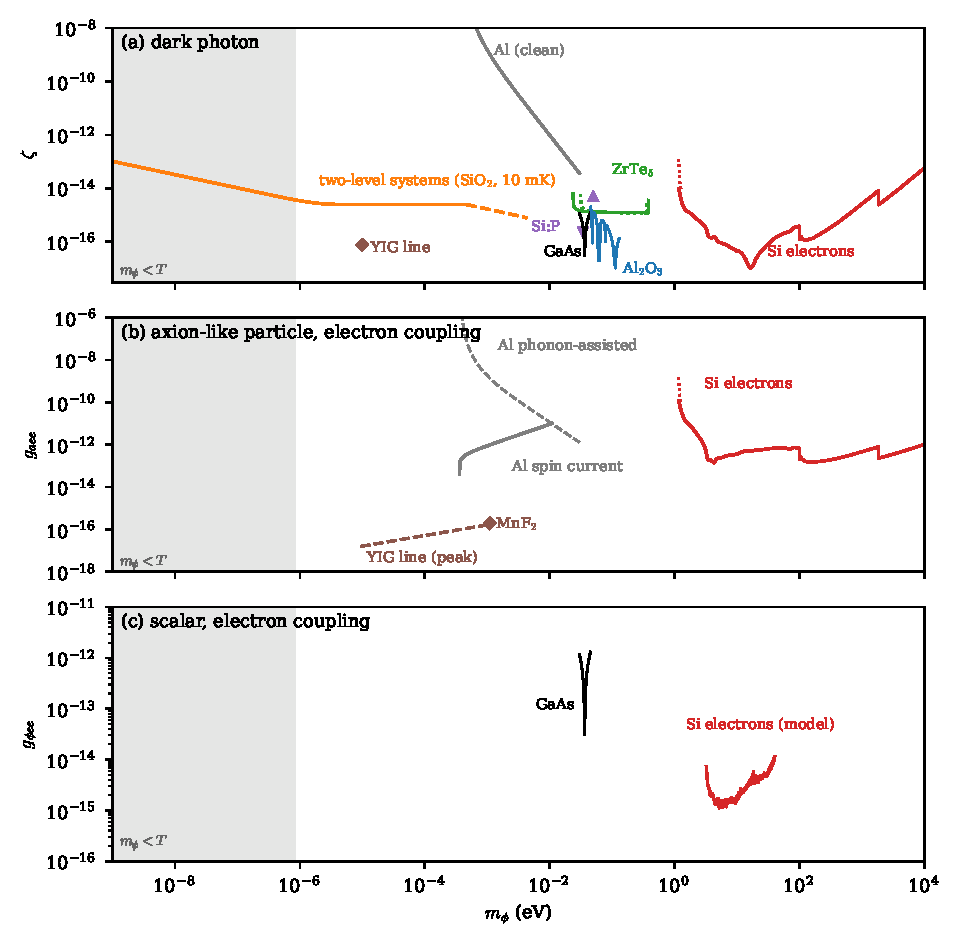
\includegraphics[width=0.86\linewidth]{figures/ch17/fig17_2.pdf}
  \caption{Absorption coverage: coupling for three events in one kilogram and year without background, $\rho_\chi = \SI{0.3}{GeV.cm^{-3}}$, against the boson mass. (a) Dark photon. Two-level systems of a thermal SiO$_2$ film at \SI{10}{mK}, $\tan\delta_0 = 3\times10^{-4}$, $\varepsilon_r = 3.9$, \cref{eq:16.7-dp} (solid, up to \SI{0.46}{meV}), and the vibrational absorption of the glass up to its Ioffe--Regel frequency, \SI{4.3}{meV} (dashed; \cref{lim:16.7d}). Clean aluminum, phonon-assisted pair creation with the Debye transport function, \cref{eq:15.4-holstein}. Si:P at \SI{e15}{cm^{-3}}: the $2p_0$ line at \SI{34.11}{meV} (down triangle) and the continuum at \SI{50}{meV} (up triangle), \cref{sec:16.5-absorption}. ZrTe$_5$ with the background in the total $\varepsilon$, polarization average, measured-structure (solid) and relaxed-cell (dotted) parameters of \cref{fig:16-zrte5}. GaAs and sapphire single-phonon lines, widths of \cref{fig:11-dpabs}. Silicon electrons from measured optical constants at \SI{300}{K} from \SI{1.1728}{eV}, with the cold excitonic edge of \cref{eq:13.8-edge} dotted up to \SI{1.3}{eV}. Diamond-shaped point: the Kittel line of a YIG sphere at \SI{10}{\micro eV}, vacuum $\zeta$, polarization random. (b) Axion-like particle, electron coupling. YIG Kittel line on resonance as it is tuned from \SI{9.5}{\micro eV} to \SI{1.16}{meV} (\SI{10}{T}), \cref{eq:14.3-peak}, and the MnF$_2$ resonance at \SI{1.1}{meV} (diamond-shaped point), both with the assumed width $\varGamma_{\mathrm{M}} = 10^{-5}\omega$. Clean aluminum: direct pair creation by the spin current, \cref{eq:15.4-sJ} with the quasiparticle factor $1/(1 + \lambda_{\mathrm{ep}}) = 0.70$, up to \SI{10.9}{meV} (solid), and the phonon-assisted $\sigma_1$ that published projections use (dashed). Silicon electrons from the measured $\sigma_1$, \cref{eq:10.7-alp}. (c) Scalar, electron coupling: the GaAs phonon line with the site couplings of \cref{eq:11.8-G}, and the kinetic-energy row of silicon in the empirical-pseudopotential model of \cref{fig:10-absorption}. Gray: $m_\phi < T$ for $T = \SI{10}{mK}$, where counting has lost its advantage over a coherent readout (\cref{sec:17.2-coherent}).}
  \label{fig:17-abs-coverage}
\end{figure}

\begin{table}[tbp]
  \centering
  \caption{Absorbing targets of the preceding chapters by decade of boson mass, with the best reach of each, three events in a kilogram and year without background. Lines are narrow and cover one mass unless tuned; continua cover the whole range given. A dash means no target in the book absorbs that boson at leading order in that decade.}
  \label{tab:17-abs-decades}
  \small
  \begin{tabular}{@{}>{\raggedright\arraybackslash}p{0.12\linewidth}>{\raggedright\arraybackslash}p{0.37\linewidth}>{\raggedright\arraybackslash}p{0.27\linewidth}>{\raggedright\arraybackslash}p{0.14\linewidth}@{}}
    \toprule
    $m_\phi$ & dark photon, $\zeta$ & axion-like, $g_{aee}$ & scalar, $g_{\phi ee}$ \\
    \midrule
    \SI{1}{neV}--\SI{1}{\micro eV} & two-level systems, $\gtrsim 3\times10^{-15}$; acoustic modes of bodies (\cref{sec:11.8-bar}); coherent readout & --- (nuclear spins couple through $g_{aNN}$, \cref{sec:14.6}) & resonant masses (\cref{sec:11.8-mass}) \\
    \SI{1}{\micro eV}--\SI{0.1}{meV} & two-level systems, $2.4\times10^{-15}$; YIG line, $7.6\times10^{-17}$ at \SI{10}{\micro eV} (vacuum $\zeta$) & YIG line, $1.6\times10^{-17}$ at \SI{10}{\micro eV} & --- \\
    \SIrange{0.1}{1}{meV} & two-level systems to \SI{0.46}{meV}, then glass vibrations; aluminum from \SI{0.36}{meV}, $1.5\times10^{-9}$ & YIG line, $1.7\times10^{-16}$ at \SI{1.16}{meV}; aluminum, $6.1\times10^{-13}$ & --- \\
    \SIrange{1}{10}{meV} & glass vibrations to \SI{4.3}{meV}, $7.6\times10^{-16}$ & MnF$_2$ line, $1.9\times10^{-16}$ at \SI{1.1}{meV}; aluminum, $9.1\times10^{-12}$ at \SI{10}{meV} & --- \\
    \SIrange{10}{100}{meV} & GaAs line, $2.9\times10^{-17}$; Si:P $2p_0$, $2.3\times10^{-16}$; ZrTe$_5$ from \SI{23.6}{meV}, $1.25\times10^{-15}$ & --- (nucleon coupling: \cref{sec:11.6}) & GaAs line, $3.1\times10^{-14}$ \\
    \SIrange{0.1}{1}{eV} & sapphire, $1.0\times10^{-17}$ at \SI{112}{meV}; ZrTe$_5$ to \SI{0.38}{eV}; none from \SIrange{0.38}{1.17}{eV} & --- & --- \\
    \SIrange{1}{10}{eV} & silicon from \SI{1.1728}{eV}; $4.4\times10^{-17}$ at \SI{10}{eV} & silicon, $1.4\times10^{-13}$ at \SI{4.3}{eV} & silicon (model), $1.1\times10^{-15}$ \\
    \SIrange{10}{100}{eV} & silicon plasmon, $1.0\times10^{-17}$ at \SI{16.4}{eV} & silicon, $3$--$5\times10^{-13}$ & silicon (model) \\
    \SIrange{0.1}{10}{keV} & silicon, $1.9\times10^{-16}$ at \SI{100}{eV}, $2.6\times10^{-15}$ at \SI{1}{keV} & silicon to \SI{1}{keV}, $3$--$5\times10^{-13}$ & --- \\
    \bottomrule
  \end{tabular}
\end{table}

The dark photon is covered almost everywhere, with two weak stretches. Between \SI{0.38}{eV}, where the Dirac cone of ZrTe$_5$ ends at twice its cutoff, and \SI{1.17}{eV}, where cold silicon begins to absorb, no target of the book absorbs at leading order; the sapphire lines and their multiphonon background end near \SI{0.12}{eV}. A narrow-gap semiconductor or a Dirac material with a wider cone would fill this gap, with the screening ceiling of its background constant. The second weak stretch is the meV decade, where the glass absorbs through its disordered vibrations at $\zeta \approx 10^{-15}$ and the superconductor is screened out.

The axion-like particle with its electron coupling has fewer targets. Magnons cover \SI{10}{\micro eV} to a meV, as far as a laboratory field tunes their lines; clean aluminum covers \SI{0.36}{meV} to \SI{11.5}{meV}, above which its phonon-assisted absorption takes over; and silicon covers everything above its edge that the tables reach. Between \SI{10}{meV} and \SI{1.17}{eV}, however, no target of the preceding chapters covers this coupling. Phonons absorb an axion-like particle through its nucleon coupling alone, on the spin-carrying isotopes of a crystal (\cref{sec:11.6}), and a Dirac material would need its spin-current response computed with its strong spin--orbit coupling, which the factor $\frac34$ of \cref{eq:10.7-alp} does not contain. The scalar has two targets: the GaAs phonon line, suppressed by the near-cancellation of its sublattices, and the kinetic row of silicon above its direct gap, which in \cref{fig:17-abs-coverage}c is a model with pseudo-wavefunctions. Between the indirect edge and \SI{3.1}{eV} silicon absorbs a scalar only with a phonon, through the kinetic row of \cref{sec:13.8}, which no measurement provides.

A tuned line and a continuum are compared differently. On resonance the Kittel line of YIG reaches $g_{aee} = 1.6\times10^{-17}$ at \SI{10}{\micro eV}, but only within its full width $\varGamma_{\mathrm{M}} = 10^{-5}m_\phi$. A search that scans the line across one e-fold of mass with uniform exposure spends a fraction $(\pi/2)\varGamma_{\mathrm{M}}/m_\phi = 1.6\times10^{-5}$ of its time on each mass. Averaged over the scan the reach is $4.1\times10^{-15}$, still a hundred times better than the continuum of clean aluminum at its best mass. The MnF$_2$ resonance at \SI{1.1}{meV} gives $1.9\times10^{-16}$ on resonance and $4.8\times10^{-14}$ averaged. The peak values rest on the assumed ratio $\varGamma_{\mathrm{M}}/\omega = 10^{-5}$ (\cref{sec:14.3}). The averaged ones do not depend on it, since the area of the line, not its height, sets what a scan delivers, as for the phonon lines of \cref{eq:11.8-Rint}. The fixed lines of GaAs, sapphire and Si:P cover their own masses alone.

\begin{workedexample}{The handover from GaAs phonons to silicon electrons}\label{we:17-handover}
GaAs absorbs a dark photon at its longitudinal optical phonon, \SI{36.35}{meV}, with all the weight of the line, $\mathcal{I}_{\mathrm{pol}} = \SI{0.759}{meV}$, within a few widths, and with multiphonon absorption up to a few phonon energies. Its electrons absorb from its gap, \SI{1.52}{eV} at low temperature (\cref{sec:3.3}). Silicon absorbs from its excitonic edge. At which mass does silicon take over?

\emph{The phonon line does not decide it.} The damped factorized model of \cref{fig:11-dpabs} gives $\varepsilon_2 = 2.5\times10^{-4}$ at \SI{1.17}{eV}, an absorption coefficient of \SI{4.3}{cm^{-1}} with the refractive index 3.48 used below. That value is an artifact of the model: with different widths in its numerator and denominator it tends to $\varepsilon_2 = \varepsilon_\infty(\gamma_{\mathrm{L}} - \gamma_{\mathrm{T}})/\omega$ far above the line, a constant conductivity. A Lorentz oscillator with a single width gives $\varepsilon_2 = 4.8\times10^{-7}$ and \SI{0.008}{cm^{-1}} at the same energy. A pure crystal transmits there, and what it absorbs depends on its defects.

\emph{Equal rates.} Per unit mass the rates are equal when $L_{\mathrm{GaAs}}/\rho_{\mathrm{GaAs}} = L_{\mathrm{Si}}/\rho_{\mathrm{Si}}$. Below a gap $\varepsilon_2 \ll \varepsilon_1 = n_r^2$, and with $\varepsilon_2 = n_r\alpha_{\mathrm{abs}}/\omega$ the loss function is $L = \alpha_{\mathrm{abs}}/(n_r^3\omega)$. With $n_r = 3.48$ for GaAs at \SI{22}{\celsius}, from the dispersion formula of Skauli et al.~\cite{skauli2003improved} as tabulated in Ref.~\cite{polyanskiy2024refractiveindex}, $n_r = 3.56$ for silicon at \SI{300}{K}~\cite{franta2017temperature}, and densities 5.361 and \SI{2.33}{g.cm^{-3}}, GaAs needs $(3.48/3.56)^3\times5.361/2.33 = 2.15$ times the absorption coefficient of silicon to match it.

\emph{The silicon edge.} At millikelvin temperatures silicon absorbs from the $1s$ replica of the transverse acoustic branch, $\Eg(0) + \omega_{\mathrm{TA}} - E_x^b = \SI{1.17277}{eV}$, and \cref{eq:13.8-edge} rises there as a square root. With the scale of \cref{sec:13.8},
\begin{equation*}
  \alpha_{\mathrm{abs}}^{\mathrm{Si}} = \SI{13.3}{cm^{-1}}\,\bigl[(m_\phi - \SI{1.17277}{eV})/\mathrm{eV}\bigr]^{1/2} ,
\end{equation*}
which is \SI{0.13}{cm^{-1}} at \SI{0.1}{meV} above the threshold and \SI{0.42}{cm^{-1}} at \SI{1}{meV}.

\emph{The handover.} Setting $2.15\,\alpha_{\mathrm{abs}}^{\mathrm{Si}}$ equal to the absorption of the GaAs crystal places the handover \SI{0.012}{meV} above the threshold for \SI{0.1}{cm^{-1}} and \SI{1.2}{meV} above it for \SI{1}{cm^{-1}}. A crystal absorbing \SI{10}{cm^{-1}} would move it \SI{40}{meV} up; at that distance the further replicas of \cref{eq:13.8-edge} have opened, and the square-root onset alone would have put it at \SI{0.12}{eV}. For any GaAs crystal transparent to better than \SI{1}{cm^{-1}}, silicon takes over within a meV of its excitonic edge, at $m_\phi \simeq \SI{1.173}{eV}$, and the square-root onset of the replica makes the handover sharp. A meV above the threshold silicon reaches $\zeta = 5.6\times10^{-14}$, two thousand times weaker than the GaAs line at its center.
\end{workedexample}

The worked example uses a model of the cold edge. The cold measurements near the edge differ among themselves by a factor of twenty (\cref{sec:13.8}), which moves the absorption of silicon but not the place of the handover, since the threshold is fixed by the gap, the phonon and the exciton binding.

\subsection{Coherent and counting readout}\label{sec:17.2-coherent}

A YIG sphere tuned to \SI{10}{\micro eV} counts the quanta it absorbs (\cref{we:14-yig}). A $^{207}$Pb sample at \SI{1}{neV} reads the transverse magnetization that the field drives (\cref{sec:14.6}). Both measure the absorptive part of a response near $\omega = m_\phi$, but the first counts quanta of energy $m_\phi$ and the second measures the amplitude of a field. Which readout is better at a given mass depends on the thermal occupation $n_{\mathrm{B}}(m_\phi) = 1/(\ee^{m_\phi/T} - 1)$ of the mode that is read, with $T$ the temperature of that mode.

Take a record of length $t_{\mathrm{int}}$ longer than the coherence time. The signal is spread over $N_{\mathrm{coh}} \simeq t_{\mathrm{int}}\Delta\omega_{\mathrm{eq}}/2\pi$ independent frequency bins, with $\Delta\omega_{\mathrm{eq}} = 2.67/t_{\mathrm{coh}}$ the equivalent width of the line (\cref{sec:14.6-stats}), and it delivers $\bar N_{\mathrm{sig}}$ absorbed quanta. A counter whose detection band is the line sees, in the same bins, $\bar N_{\mathrm{th}} = n_{\mathrm{B}}(m_\phi)N_{\mathrm{coh}}$ thermal quanta. They are chaotic, and their number fluctuates with the variance $\bar N_{\mathrm{th}} + \bar N_{\mathrm{th}}^2/N_{\mathrm{coh}} = N_{\mathrm{coh}}n_{\mathrm{B}}(m_\phi)[n_{\mathrm{B}}(m_\phi) + 1]$ of \cref{sec:14.6-regime}. A linear readout, a phase-preserving amplifier or a magnetometer, measures both quadratures of the mode, and its noise is at least $n_{\mathrm{B}}(m_\phi) + 1$ quanta per bin: the thermal quanta plus one zero-point quantum, half of it present at the input and half added by the amplifier~\cite[Eq.~(9)]{lamoreaux2013analysis}. This per-bin noise has the rms $n_{\mathrm{B}}(m_\phi) + 1$, and summed in quadrature over the bins it fluctuates by $[n_{\mathrm{B}}(m_\phi) + 1]N_{\mathrm{coh}}^{1/2}$. The significance of the signal is then $\bar N_{\mathrm{sig}}/\{N_{\mathrm{coh}}n_{\mathrm{B}}(m_\phi)[n_{\mathrm{B}}(m_\phi) + 1]\}^{1/2}$ for the counter and $\bar N_{\mathrm{sig}}/\{N_{\mathrm{coh}}^{1/2}[n_{\mathrm{B}}(m_\phi) + 1]\}$ for the linear readout, whose square is the weak-signal statistic $\mathsf{t}$ of \cref{sec:14.6-stats} with $x_k = \bar N_{\mathrm{sig}}/\{N_{\mathrm{coh}}[n_{\mathrm{B}}(m_\phi) + 1]\}$ in each bin. At equal significance the counter needs fewer signal quanta by the ratio
\begin{keyresult}[Counting against linear readout]
\begin{equation}
  \frac{\bar N_{\mathrm{sig}}^{\mathrm{lin}}}{\bar N_{\mathrm{sig}}^{\mathrm{cnt}}} = \Bigl[\frac{n_{\mathrm{B}}(m_\phi) + 1}{n_{\mathrm{B}}(m_\phi)}\Bigr]^{1/2} = \ee^{m_\phi/2T} ,
  \label{eq:17.2-ratio}
\end{equation}
for the same absorber, record and line, as long as the counter sees thermal quanta in the record and its detection band is the line width $\Delta\omega_{\mathrm{eq}}$. A counter that sees a band $B$ wider than the line collects more thermal quanta, and the ratio is multiplied by $(B/\Delta\omega_{\mathrm{eq}})^{-1/2}$. In the coupling, which enters the signal squared, the ratio is $\ee^{m_\phi/4T}$. For $n_{\mathrm{B}}(m_\phi) \ll 1$ the Poisson treatment of Lamoreaux and collaborators~\cite[Eqs.~(12)--(14)]{lamoreaux2013analysis} is the limit of this result; their cavity counter sees the whole cavity band, which carries the extra factor $(Q_{\mathrm{c}}/2\pi Q_a)^{1/2}$ of their Eq.~(18), with $Q_{\mathrm{c}}$ and $Q_a$ the quality factors of the cavity and of the line.
\end{keyresult}

Three regimes follow. For $m_\phi \ll T$ the ratio tends to one. Each mode holds many thermal quanta, their fluctuation dominates either readout, and a counter gains nothing over a measurement of the field, while it would have to resolve single quanta far below the thermal energy. At \SI{1}{neV} a mode at \SI{4.2}{K} holds $3.6\times10^5$ quanta and one at \SI{10}{mK} holds 861, and every search there reads the field. For $m_\phi \approx T$ the gain is modest, 1.65 in the signal and 1.28 in the coupling at $m_\phi = T$. For $m_\phi \gg T$ the counter wins exponentially, until the record holds no thermal quantum at all. Requiring zero thermal counts with \SI{95}{\percent} probability, $\bar N_{\mathrm{th}} < 0.05$, the counter needs three signal quanta (\cref{sec:1.5})~\cite[Eqs.~(19), (20)]{lamoreaux2013analysis}, whatever the mass. With $\Delta\omega_{\mathrm{eq}} = 2.67\,m_\phi v_0^2$ this happens above \SI{17}{\micro eV} for a one-hour record and \SI{20}{\micro eV} (\SI{4.9}{GHz}) for one day at \SI{10}{mK}, and above \SI{0.19}{meV} and \SI{0.22}{meV} at \SI{100}{mK}, that is, at $m_\phi \approx (20$--$26)\,T$. The linear readout still needs $\bar N_{\mathrm{sig}} = (2.71\,N_{\mathrm{coh}})^{1/2}[n_{\mathrm{B}}(m_\phi) + 1]$ at the threshold $\mathsf{t} = 2.71$ of \cref{eq:C.14-thresholds}, the one-sided \SI{95}{\percent} level. For instance, at \SI{24.8}{\micro eV}, the 6-GHz mass of \cref{we:16-tls-dp}, a day at \SI{10}{mK} spreads the line over $8.7\times10^8$ bins, and the linear readout needs $4.9\times10^4$ quanta against the counter's three, a factor of 127 in the coupling. At \SI{10}{\micro eV} the same record still holds 3200 thermal quanta, and the counter wins by 330 in the signal and 18 in the coupling.

The gray band of \cref{fig:17-abs-coverage}, $m_\phi < T$ (\SI{0.86}{\micro eV}, or \SI{210}{MHz} at \SI{10}{mK}), is where the advantage of counting has fallen below $\ee^{1/2}$ and tends to one, and the field is read coherently. Above that mass the counter gains $\ee^{m_\phi/4T}$ in the coupling, and above $20\,T$ it is limited by the absorbed quanta alone, with a reach that improves as $t_{\mathrm{int}}^{-1/2}$ against the $(t_{\mathrm{int}}t_{\mathrm{coh}})^{-1/4}$ of the field measurement (\cref{eq:14.6-scaling}). Two effects reduce the advantage. A linear readout of one quadrature of a squeezed mode can go below one zero-point quantum~\cite{lamoreaux2013analysis}, which narrows the gap by the degree of squeezing. A real counter, moreover, has dark counts besides the thermal quanta, and they add to its background. The background-free counting that the reach curves of \cref{fig:17-abs-coverage} assume holds where both are absent.

\section{Inelastic scattering into collective modes}\label{sec:17.3}

A dark-matter particle of \SI{10}{keV} at the largest laboratory speed $v_{\mathrm{max}}$ carries \SI{35}{meV} of kinetic energy, just short of the \SI{36.35}{meV} longitudinal optical phonon of GaAs, and elastic scattering cannot create that phonon below \SI{10.35}{keV} (\cref{sec:11.2}). Let the same particle arrive in an excited state \SI{1}{eV} above its ground state and leave in the lower one. It then emits the phonon at every speed of the halo, at a rate of $2.6\times10^4$ events per kilogram and year for a light dark photon at $\sigmae = \SI{e-40}{cm^2}$. \Cref{sec:10.9} followed the splitting $\Delta_\chi$ through the electron-recoil spectrum of silicon. The collective modes, phonons, magnons and plasmons, are the natural final states of down-scattering (\cref{sec:8.2-exothermic}): the band of allowed $(\vect{q},\omega)$ moves up by $|\Delta_\chi|$, and a mode whose energy lies below the splitting is always reached. One formula covers all the modes, and the dispersion of each mode decides where its line lies, how wide it is, and how much of the splitting it takes.

\subsection{Down-scattering into a collective mode}\label{sec:17.3-shell}

Every collective response of \cref{chap:10,chap:11,chap:14} is, at $T = 0$, a sum of lines. The one-phonon response \cref{eq:11.1-S1}, the one-magnon response \cref{eq:14.1-Safm} and the plasmon pole of \cref{eq:4.5-plasmonL} each put a weight on the dispersion surface $\omega = \omega_\nu(\vect{q})$ of a branch $\nu$. Contracted with the dark-matter tensor, the integrand of \cref{eq:8.2-spectrum} becomes
\begin{equation}
  \sum_{ab}\mathfrak{D}_{ab}(\vect{q})\,S_{ab}(\vect{q},\omega) = \frac{2\pi}{\Omega}\sum_\nu\mathcal{Y}_\nu(\vect{q})\,\delta\bigl(\omega - \omega_\nu(\vect{q})\bigr) ,
  \label{eq:17.3-lines}
\end{equation}
which defines the mode weight $\mathcal{Y}_\nu \ge 0$. For the nucleon coupling of \cref{sec:11.1}, in the notation of \cref{eq:11.1-S1} (nucleon numbers $A_\kappa$, polarization vectors $\vect{e}_{\kappa\nu}$), $\mathcal{Y}_\nu = |\tilde V_N|^2|\sum_\kappa A_\kappa\ee^{-W_\kappa}\ee^{\ii\vect{q}\cdot\vect{\tau}_\kappa}\vect{q}\cdot\vect{e}^*_{\kappa\nu}/\sqrt{M_\kappa}|^2/2\omega_\nu$. For the spin coupling $\mathcal{O}_4$ in an antiferromagnet, with $\Omega = \Omega_{\mathrm{ion}}$, the contraction \cref{eq:14.1-contract} gives $\mathcal{Y} = \tfrac14|\vect{S}||c_4|^2|F^{\mathrm{mag}}|^2w^{\mathrm{M}}_{\vect{q}}$, with the coupling $c_4$, the magnetic form factor $F^{\mathrm{mag}}$ and the magnon weight $w^{\mathrm{M}}_{\vect{q}}$ of \cref{sec:14.1}. For the plasmon of an electron gas coupled through the electron density, $S = (2q^2/e^2)L$ and the pole carries the weight $\pi/(\partial\varepsilon_1/\partial\omega)$, so that $\mathcal{Y} = \Omega|\tilde V|^2q^2/[e^2\,\partial\varepsilon_1/\partial\omega]$.

Down-scattering has $\Delta_\chi < 0$, and energy conservation, $\omega_{\vect{q}} = \omega_\nu(\vect{q})$ with $\omega_{\vect{q}}$ of \cref{eq:1.3-omegaq}, reads
\begin{equation*}
  |\Delta_\chi| + \vect{q}\cdot\vect{v} - \frac{q^2}{2\mchi} = \omega_\nu(\vect{q}) .
\end{equation*}
We first set $\vect{v} = 0$. Along each direction $\hat{\vect{q}}$ the condition fixes the magnitude of the momentum transfer at the roots $q_\nu(\hat{\vect{q}})$ of
\begin{equation}
  |\Delta_\chi| - \frac{q_\nu^2}{2\mchi} = \omega_\nu(q_\nu\hat{\vect{q}}) ,
  \label{eq:17.3-qnu}
\end{equation}
and we write $v_\nu = q_\nu/\mchi$ for the speed of the outgoing particle relative to the incoming one. For a mode whose energy is small against the splitting, $q_\nu \simeq (2\mchi|\Delta_\chi|)^{1/2}$; at a fixed deposit $\omega$ this is the shell momentum $q_\Delta$ of \cref{sec:10.9}. As a function of $q$ along $\hat{\vect{q}}$, the argument of the delta function has the slope $-(q/\mchi + u_\nu)$, with $u_\nu = \hat{\vect{q}}\cdot\nabla_{\vect{q}}\,\omega_\nu$ the group velocity of the mode along $\vect{q}$. Writing $\dd^3q = q^2\dd q\,\dd^2\hat{\vect{q}}$, the radial integral picks up $q_\nu^2/(q_\nu/\mchi + u_\nu)$ at each root. The rate of one particle, $\varGamma = \int\dd\omega\int\dd^3q/(2\pi)^3\,\sum\mathfrak{D}_{ab}S_{ab}\,\delta(\omega - \omega_{\vect{q}})$, is then $(2\pi)^{-3}(2\pi/\Omega)\sum_\nu\int\dd^2\hat{\vect{q}}\,q_\nu^2\mathcal{Y}_\nu/(q_\nu/\mchi + u_\nu)$, which summed over branches and directions reads
\begin{keyresult}[Exothermic rate into a collective mode]
\begin{equation}
  \varGamma = \frac{\mchi}{\pi\Omega}\sum_\nu\Bigl\langle\frac{q_\nu\,\mathcal{Y}_\nu(q_\nu\hat{\vect{q}})}{1 + u_\nu/v_\nu}\Bigr\rangle_{\hat{\vect{q}}}\Bigl[1 + O\bigl(v^2/v_\nu^2\bigr)\Bigr] , \qquad
  \mathcal{R} = \frac{\rho_\chi}{\mchi\rho_T}\,\varGamma ,
  \label{eq:17.3-rate}
\end{equation}
with $q_\nu$ the roots of \cref{eq:17.3-qnu}, $\langle\cdot\rangle_{\hat{\vect{q}}}$ the average over directions, and $\mathcal{R}$ the rate per unit target mass. It holds for $v_\nu$ above the speeds of the halo and for a weight $\mathcal{Y}_\nu$ that varies little over momenta $\mchi v_{\mathrm{max}}$.
\end{keyresult}
\noindent At finite $\vect{v}$ the surface of \cref{eq:17.3-qnu} moves by a vector of order $\mchi\vect{v}$ and changes its radius at second order. The term linear in $\vect{v}$ averages to zero over a weight and a dispersion even in $\vect{q}$, as for the electronic shell of \cref{eq:10.9-shell}, and the correction to the rate is of order $v^2/v_\nu^2$. The deposited energy, by contrast, shifts at first order, and \cref{sec:17.3-lines} shows that this sets the width of the line. The factor $(1 + u_\nu/v_\nu)^{-1}$ is new compared with the electronic shell, where the energy is integrated at fixed $\omega$. It is close to one for phonons and magnons, whose group velocities, $10^{-5}$ to $10^{-4}$, lie far below $v_\nu$, but not for the plasmon, whose dispersion is steep.

The velocity independence has a simple reading in the incoherent limit. For a free scatterer the rate per particle of elastic scattering is $\nd\sigma v$, and that of exothermic down-scattering is $\nd\sigma v_\nu$: the final momentum, and with it the phase space, is fixed by the splitting rather than by the incoming speed. The magnons of NiO show it. With the spin coupling $\mathcal{O}_4$, a heavy mediator and $\sigmae = \SI{e-40}{cm^2}$ (the setting of \cref{fig:14-nio-rate}), a particle of \SI{1}{MeV} with $|\Delta_\chi| = \SI{10}{eV}$ has $q_\nu = \SI{4.45}{keV}$, beyond the ordering wavevector at \SI{2.58}{keV}. The shell then crosses many magnetic zones, and the direction average of the weight is 1.149, close to its zone average 1.156 (in the spin-wave theory of \cref{we:14-nio}, $1 + 2\Delta S = 1.157$, with $\Delta S$ the zero-point spin reduction). \Cref{eq:17.3-rate} yields 8210 events per kilogram and year, within \SI{3}{\percent} of the full integral over the halo, 8000, against 2620 for elastic scattering at the same mass.

\subsection{Line positions and widths}\label{sec:17.3-lines}

Each root of \cref{eq:17.3-qnu} deposits $\omega_\nu(q_\nu\hat{\vect{q}})$. The splitting is shared between the outgoing dark matter, which keeps $q_\nu^2/2\mchi$, and the mode, and the dispersion decides the share. A parabolic branch, $\omega_\nu(\vect{q}) = \omega_\nu(0) + q^2/2m^*_\nu$ with a dispersion mass $m^*_\nu$ of either sign, makes this exact for any $\vect{v}$. Energy conservation becomes $|\Delta_\chi| - \omega_\nu(0) + \vect{q}\cdot\vect{v} = q^2/2\mu_\nu$ with $\mu_\nu = \mchi m^*_\nu/(\mchi + m^*_\nu)$, and completing the square,
\begin{gather}
  |\vect{q} - \mu_\nu\vect{v}|^2 = q_\nu^2 + \mu_\nu^2v^2 , \qquad
  q_\nu^2 = 2\mu_\nu\bigl(|\Delta_\chi| - \omega_\nu(0)\bigr) , \notag\\
  \omega_\nu(q_\nu) = \omega_\nu(0) + \frac{\mu_\nu}{m^*_\nu}\bigl(|\Delta_\chi| - \omega_\nu(0)\bigr) .
  \label{eq:17.3-parabolic}
\end{gather}
The momentum transfers lie on a sphere centered at $\mu_\nu\vect{v}$, and at $\vect{v} = 0$ the mode takes the fraction $\mu_\nu/m^*_\nu = \mchi/(\mchi + m^*_\nu)$ of the energy above its bottom. A free electron at rest is the branch $\omega(0) = 0$, $m^* = m_e$, and \cref{eq:17.3-parabolic} returns the line $(\mu_{\chi e}/m_e)|\Delta_\chi|$ of \cref{sec:10.9-inelastic}. A flat branch, $|m^*_\nu| \gg \mchi$, takes little more than $\omega_\nu(0)$ and leaves the rest of the splitting to the dark matter. A steep branch, $m^*_\nu \ll \mchi$, takes nearly all of it.

The width follows from the same sphere. On it $q^2 = q_\nu^2 + 2\mu_\nu^2v^2 + 2\mu_\nu\vect{v}\cdot(\vect{q} - \mu_\nu\vect{v})$, and the deposited energy $\omega_\nu(0) + q^2/2m^*_\nu$ differs from the line $\omega_\nu(q_\nu)$ by $(\mu_\nu q_\nu v/m^*_\nu)\cos\theta$ plus a shift of order $v^2$, with $\theta$ the angle between $\vect{v}$ and $\vect{q} - \mu_\nu\vect{v}$. For a weight that is the same in every direction, $\cos\theta$ is uniform on the sphere, and a particle of speed $v$ spreads its energy uniformly over a band of full width $2\mu_\nu q_\nu v/|m^*_\nu|$. Averaging over the halo with the factor $1/v$ of this normalization turns the band into $\eta$:
\begin{equation}
  \frac{1}{\varGamma_\nu}\frac{\dd\varGamma_\nu}{\dd\omega} = \frac{|m^*_\nu|}{2\mu_\nu q_\nu}\;\eta\Bigl(\frac{|m^*_\nu|\,|\omega - \omega_\nu(q_\nu)|}{\mu_\nu q_\nu}\Bigr) ,
  \label{eq:17.3-profile}
\end{equation}
to first order in $v/v_\nu$, normalized by $\int_0^\infty\eta(u)\,\dd u = 1$. The line has the shape of $\eta(\vmin)$ reflected about its center. It is flat near the center, where every particle contributes, falls to half height where $\eta$ does, at \SI{278}{km/s} or 0.35 of $v_{\mathrm{max}}$, and ends at the full width $2\mu_\nu q_\nu v_{\mathrm{max}}/|m^*_\nu|$. For a branch that is not parabolic, the same steps with the dispersion linearized about $q_\nu$ replace $q_\nu/m^*_\nu$ by $u_\nu$ and $\mu_\nu$ by $\mchi$, as long as $|u_\nu| \ll v_\nu$: the full width is $2|u_\nu|\mchi v_{\mathrm{max}}$. Intrinsic widths of the mode, from anharmonic decay of a phonon or Landau and interband damping of a plasmon, add by convolution.

An acoustic branch, $\omega = c_\nu q$, has $q_\nu = \mchi[(c_\nu^2 + 2|\Delta_\chi|/\mchi)^{1/2} - c_\nu]$ and a line at $c_\nu q_\nu$ whose full width relative to its energy is $2v_{\mathrm{max}}/v_\nu$. It is a line as long as $v_\nu$ is well above $v_{\mathrm{max}}$ and $q_\nu$ still lies inside the zone. Antiferromagnetic magnons near $\Gamma$ behave the same way. In NiO at \SI{0.1}{MeV} and $|\Delta_\chi| = \SI{1}{eV}$, $q_\nu = \SI{435}{eV}$, and the magnons emitted at $\vect{v} = 0$ have \SI{55.1}{meV} with a spread of \SI{0.9}{meV} over directions. However, $v_{\mathrm{max}}/v_\nu = 0.61$, and with the mean group velocity $1.1\times10^{-4}$ the halo spreads them over a full width $2|u_\nu|\mchi v_{\mathrm{max}} = \SI{60}{meV}$, more than the line energy. Their weight there, 0.28 on average, includes the suppression near $\Gamma$ of \cref{sec:14.1}, and \cref{eq:17.3-rate} yields 5130 events per kilogram and year against 5710 from the full integral and 434 for elastic scattering. Once $q_\nu$ crosses many zones, the deposited energies sample the whole branch, and the spectrum becomes the weighted density of states: \SI{100}{meV} on average, with a spread of \SI{15}{meV}, for NiO at \SI{1}{MeV} and $|\Delta_\chi| = \SI{10}{eV}$.

The magnons of a ferromagnet start at the Larmor frequency and disperse quadratically near $\Gamma$, a parabolic branch with $\omega_\nu(0) = \omega_{\mathrm{Lar}}$ and a positive $m^*_\nu$. As $|\Delta_\chi|$ approaches $\omega_{\mathrm{Lar}}$, $q_\nu \to 0$ and \cref{eq:17.3-rate} vanishes in proportion to $q_\nu$ for a coupling without $q$ dependence. The uniform precession of \cref{sec:14.3} is the end point of the exothermic spectrum, where the halo speeds take over from the splitting.

A flat optical branch gives a narrow line at its own energy, and \cref{we:17-gaas} works it out for GaAs.

The plasmon is the steep case. Expanding the gas dispersion of \cref{sec:4.5}, $\omega_{\mathrm{pl}} \simeq \omega_p + \alpha_{\mathrm{pl}}q^2/m_e$, gives $m^*_{\mathrm{pl}} = m_e/2\alpha_{\mathrm{pl}}$. At the valence density of silicon, $E_{\mathrm{F}} = \SI{12.47}{eV}$, $\omega_p = \SI{16.61}{eV}$ and $\alpha_{\mathrm{pl}} = \tfrac35E_{\mathrm{F}}/\omega_p = 0.451$, so that $m^*_{\mathrm{pl}} = \SI{567}{keV}$, lighter than the dark matter of most electron-recoil searches. A particle of \SI{1}{MeV} has $\mu_{\mathrm{pl}} = \SI{362}{keV}$ and hands the plasmon 0.638 of the splitting above $\omega_p$, a particle of \SI{10}{MeV} 0.946. At $|\Delta_\chi| = \SI{20}{eV}$ and \SI{1}{MeV}, \cref{eq:17.3-parabolic} puts the line at \SI{18.77}{eV} and $q_\nu = \SI{1.57}{keV}$, and the exact zero of the Lindhard function at \SI{18.83}{eV} and \SI{1.53}{keV}. The steep dispersion that hands the plasmon the splitting also makes the line wide: the full width from the halo is \SI{5.3}{eV}, more than the measured \SI{3.66}{eV} width of the silicon loss peak (\cref{sec:4.5}). Since the plasmon exists only below the Landau-damping momentum, the line exists only in a window of splittings. The parabolic dispersion meets the upper edge of the pair continuum, $qv_{\mathrm{F}} + q^2/2m_e$, at \SI{2.30}{keV}, and the window closes \SI{7.3}{eV} above $\omega_p$ at \SI{1}{MeV}.

\begin{workedexample}{Exothermic emission of an optical phonon in GaAs}\label{we:17-gaas}
Take a dark photon, $\sigmae = \SI{e-40}{cm^2}$ as in \cref{sec:11.2}, $\mchi = \SI{30}{keV}$ and $\Delta_\chi = \SI{-1}{eV}$. The splitting lies below the gap of GaAs, \SI{1.52}{eV}, so no electronic excitation is open, and the dark photon reaches the lattice through the longitudinal optical phonon alone. Its line in the loss function carries $(\pi\omega_{\mathrm{L}}/2)(1 - \omega_{\mathrm{T}}^2/\omega_{\mathrm{L}}^2)/\varepsilon_\infty = \SI{7.59e-4}{eV}$ with the measured $\omega_{\mathrm{T}} = \SI{33.62}{meV}$, $\omega_{\mathrm{L}} = \SI{36.35}{meV}$ and $\varepsilon_\infty = 10.88$ (\cref{eq:11.2-onebranch}, splitting route). With this line in place of the averaged loss function $\bar L$ of \cref{eq:10.9-shell}, that equation times $(1 + u_\nu/v_\nu)^{-1}$ is \cref{eq:17.3-rate} for the charge coupling:
\begin{equation*}
  \mathcal{R} = \frac{\rho_\chi\,\sigmae\,q_\nu^3\,\FDM(q_\nu)^2\,\omega_{\mathrm{L}}}{2e^2\rho_T\,\mu_{\chi e}^2}\,\frac{1}{\varepsilon_\infty}\Bigl(1 - \frac{\omega_{\mathrm{T}}^2}{\omega_{\mathrm{L}}^2}\Bigr)\frac{1}{1 + u_\nu/v_\nu} .
\end{equation*}

\emph{Kinematics.} With the computed dispersion of the longitudinal branch of \cref{sec:5.5}, shifted to the measured $\omega_{\mathrm{L}}$ at $\Gamma$ and averaged over $[100]$, $[110]$ and $[111]$, \cref{eq:17.3-qnu} gives $q_\nu = \SI{240.5}{eV}$, 0.109 of $2\pi/a$ and inside the region where the Born-charge vertex holds (\cref{sec:11.2}). Then $v_\nu = 8.0\times10^{-3}$ and $v_{\mathrm{max}}/v_\nu = 0.33$. The estimate $2.5\langle v^2\rangle/v_\nu^2$ of \cref{sec:10.9} puts the halo correction to the rate at \SI{6}{\percent}.

\emph{Line.} The branch falls with $q$, $u_\nu = -6.2\times10^{-7}$, and the line lies at \SI{36.279}{meV}, \SI{0.071}{meV} below $\omega_{\mathrm{L}}$, between 36.256 and \SI{36.314}{meV} depending on the direction. Its full width from the halo, $2|u_\nu|\mchi v_{\mathrm{max}}$, is \SI{0.099}{meV}, and its half-maximum width 0.35 of that. Both are below the anharmonic width of the phonon, a fraction of a meV (\cref{sec:11.2}). The dark matter keeps \SI{0.964}{eV}; the detector sees one optical phonon.

\emph{Rate.} For a light dark photon, $\FDM = (q_0/q)^2$, the formula yields 1817 events per kilogram and year, and the full integral over the halo with the absolute value in $\vmin$ (\cref{eq:10.9-inel}) 1810. Elastic scattering at the same mass leads to 842, so the splitting doubles the rate while fixing the energy deposited. For a heavy dark photon the shell form is at 0.0314 and the full integral 0.0334, against $5.7\times10^{-5}$ for elastic scattering, a gain of 585. The two mediators respond oppositely to the splitting, since the light one weights $q_\nu^{-1}$ and the heavy one $q_\nu^3$. At $|\Delta_\chi| = \SI{0.5}{eV}$ the full integrals give 2600 for the light dark photon and 0.012 for the heavy one; the shell form yields 2620 and 0.010, off by \SI{12}{\percent} for the heavy mediator, which weights the largest momenta, at $v_{\mathrm{max}}/v_\nu = 0.48$.

\emph{Below the elastic edge.} At \SI{10}{keV}, under the edge $2\omega_{\mathrm{L}}/v_{\mathrm{max}}^2 = \SI{10.35}{keV}$, elastic scattering is closed. The same splitting gives $q_\nu = \SI{138.8}{eV}$, $v_{\mathrm{max}}/v_\nu = 0.19$, and $2.6\times10^4$ events per kilogram and year for the light dark photon, with the shell form within \SI{0.1}{\percent} of the full integral.
\end{workedexample}

\subsection{Electronic and collective channels in silicon}\label{sec:17.3-silicon}

\begin{figure}[tbp]
  \centering
  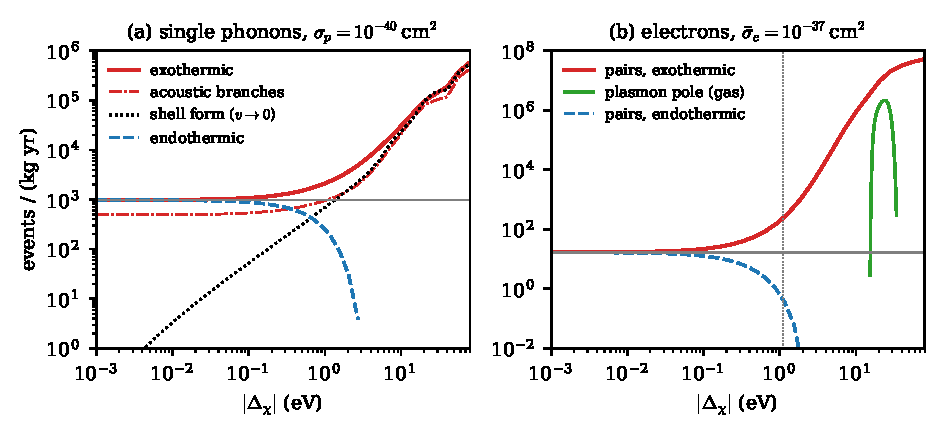
\includegraphics[width=\linewidth]{figures/ch17/fig17_3.pdf}
  \caption{Rates of silicon per kilogram and year against the mass splitting for $\mchi = \SI{1}{MeV}$, heavy mediator, standard halo of \cref{sec:1.2}, $T = 0$. Solid: exothermic ($\Delta_\chi = -|\Delta_\chi|$); dashed: endothermic ($\Delta_\chi = +|\Delta_\chi|$); gray line: elastic scattering. (a) Single phonons for a coupling to the nucleon number, $\sigma_p = \SI{e-40}{cm^2}$: the one-phonon response \cref{eq:11.1-S1} with all six branches of the computed phonons of \cref{sec:5.2} at the actual $\vect{q}$ (Umklapp and Debye--Waller factor included), averaged over the orientations of the crystal, deposits $\omega \ge \SI{1}{meV}$; dash-dotted: the three lowest branches; dotted: the shell form \cref{eq:17.3-rate}. (b) Electrons for a coupling to the electron density, $\sigmae = \SI{e-37}{cm^2}$: pairs from \cref{eq:10.9-inel} with the random-phase loss function with local fields of the tables of \cref{sec:10.2}, above \SI{1.11}{eV}, the step-model gap of their package (dotted vertical line; the tables are scissored to \SI{1.17}{eV}, \cref{sec:10.10}), the loss function held at its first tabulated momentum, \SI{493}{eV}, below it; green: the plasmon pole of an electron gas at the valence density of silicon, \cref{eq:10.3-plrate} with the splitting in $\vmin$, a model of the plasmon part of the electronic rate.}
  \label{fig:17-exo}
\end{figure}

\Cref{fig:17-exo} puts the two couplings of silicon side by side at \SI{1}{MeV}, each at its reference cross-section. Their elastic rates are 976 events per kilogram and year for single phonons and 16.7 for pairs. A particle of that mass carries up to $\tfrac12\mchi v_{\mathrm{max}}^2 = \SI{3.51}{eV}$, and a splitting well below this changes little: at $|\Delta_\chi| = \SI{0.12}{eV}$ the two rates are 1.12 and 1.39 times their elastic values. Above a few eV the splitting dominates, and the two channels respond to it differently.

The single-phonon rate rises from $2.0\times10^3$ at \SI{0.94}{eV} to $3.2\times10^4$ at \SI{10.3}{eV} and $5.8\times10^5$ at \SI{80}{eV}. The momentum transfer $q_\nu \simeq (2\mchi|\Delta_\chi|)^{1/2}$ grows from \SI{1.4}{keV} to \SI{12.6}{keV}, from $0.6$ to $5.6\,q_{\mathrm{BZ}}$. The one-phonon weight grows as $q^2$ times the Debye--Waller factor, whose exponent $2W$ is still just 0.10 at \SI{80}{eV}; two-phonon emission is smaller than one-phonon emission by a factor of order $W$. The deposited energy does not follow the splitting. Beyond the zone the shell crosses every branch, the spectrum is the weighted density of phonon states, and at \SI{10}{eV} the mean deposit is \SI{34.5}{meV}, with \SI{42}{\percent} above \SI{40}{meV} in the optical branches. A detector reading phonons sees the same energies as for elastic scattering, with a rate raised by a factor of 31 at \SI{10}{eV}. Between 10.3 and \SI{80}{eV} the shell form lies at 0.78 to 1.10 of the full integral. The residual comes from the condition on the weight in \cref{eq:17.3-rate}, not from the halo speeds, whose correction is $(v_{\mathrm{max}}/v_\nu)^2 \le 0.34$ there: the one-phonon weight varies on the scale $q_{\mathrm{BZ}} = \SI{2.25}{keV}$, smaller than $\mchi v_{\mathrm{max}} = \SI{2.65}{keV}$, and a single momentum per direction misses that structure.

The electronic rate rises far more steeply, from 165 at \SI{0.94}{eV} to $9.6\times10^5$ at \SI{10.3}{eV} and $5.3\times10^7$ at \SI{80}{eV}, a gain of $3\times10^6$ over the elastic rate. Elastic scattering at \SI{1}{MeV} barely crosses the gap, so any energy the splitting adds opens phase space that was nearly closed. Here the deposit does follow the splitting: \cref{sec:10.9} found the spectrum peaked between the gap and the plasma frequency, where $q_\Delta^3\bar L$ is largest, and an electronic detector reads energies of order $|\Delta_\chi|$.

The plasmon pole opens inside the electronic channel. For the electron gas at \SI{1}{MeV} it requires $\omega_{\mathrm{pl}}(q) - qv_{\mathrm{max}} + q^2/2\mchi \le |\Delta_\chi|$ at some $q$ below the Landau-damping momentum; the minimum is \SI{15.4}{eV}, above the \SI{14.7}{eV} found for a heavy particle in \cref{sec:10.3}, since a particle of \SI{1}{MeV} keeps $q^2/2\mchi$. The pole rate then grows to $2.2\times10^6$ events per kilogram and year at $|\Delta_\chi| = \SI{23.8}{eV}$ and falls beyond, as $q_\nu$ approaches the damping momentum and the weight of the line goes to zero. Between 18 and \SI{22}{eV} it is 0.09 to 0.16 of the electronic rate of the tables. The two are different models, an undamped pole in a gas against a broad loss peak in a crystal; in both, the plasmon is a minority share of exothermic electron recoil even where it is open. In a detector the plasmon decays into pairs (\cref{sec:10.3-decay}), and its line, \SI{5.3}{eV} wide from the halo alone at \SI{20}{eV}, merges with the pair spectrum around it.

\subsection{Endothermic thresholds}\label{sec:17.3-endo}

An endothermic splitting is supplied by the kinetic energy, and every channel acquires a lightest mass. For a mode with a gap and a parabolic dispersion, \cref{eq:17.3-parabolic} with $\Delta_\chi > 0$ gives $\vmin = (\Delta_\chi + \omega_\nu(0))/q + q/2\mu_\nu$. It is smallest at $q = [2\mu_\nu(\Delta_\chi + \omega_\nu(0))]^{1/2}$, and a particle at $v_{\mathrm{max}}$ reaches the mode if
\begin{equation}
  \mu_\nu \ge \frac{2\bigl(\Delta_\chi + \omega_\nu(0)\bigr)}{v_{\mathrm{max}}^2} .
  \label{eq:17.3-endogap}
\end{equation}
For a flat branch $\mu_\nu = \mchi$, and this is \cref{eq:1.3-mmin} with $\omega_{\mathrm{th}} \to \Delta_\chi + \omega_\nu(0)$; electron--hole pairs follow with $\omega_\nu(0) \to \Eg$, as in \cref{sec:10.9-inelastic}. For a gapless linear branch with a threshold $\omega_{\mathrm{th}}$, $\vmin = \Delta_\chi/q + c_\nu + q/2\mchi$ must fall below $v_{\mathrm{max}}$ at some $q \ge \omega_{\mathrm{th}}/c_\nu$. Its unconstrained minimum lies at $q = (2\mchi\Delta_\chi)^{1/2}$, and
\begin{equation}
  \mchi \ge
  \begin{cases}
    \dfrac{2\Delta_\chi}{(v_{\mathrm{max}} - c_\nu)^2} , & (2\mchi\Delta_\chi)^{1/2} \ge \omega_{\mathrm{th}}/c_\nu , \\[1.5ex]
    \dfrac{\omega_{\mathrm{th}}}{2c_\nu\bigl(v_{\mathrm{max}} - c_\nu - c_\nu\Delta_\chi/\omega_{\mathrm{th}}\bigr)} , & \text{otherwise} .
  \end{cases}
  \label{eq:17.3-endolin}
\end{equation}
At $\Delta_\chi = 0$ the momentum threshold always binds, and \cref{eq:17.3-endolin} reduces to the acoustic edge \cref{eq:11.1-edge} and its magnon analog \cref{eq:14.1-mmin}.

\begin{table}[tbp]
  \centering
  \caption{Lightest dark-matter mass that reaches each channel for the endothermic splittings $\Delta_\chi = 0$, \SI{10}{meV} and \SI{1}{eV}, from \cref{eq:17.3-endogap,eq:17.3-endolin} with $v_{\mathrm{max}} = 2.650\times10^{-3}$. Gapped channels: the low-temperature gap of silicon, \SI{1.17}{eV}; the optical phonon of silicon at \SI{64.1}{meV} (\cref{sec:5.2}); the longitudinal optical phonon of GaAs at \SI{36.35}{meV} (\cref{we:5-lst}). Linear channels: the largest longitudinal sound speed of silicon, \SI{9.35}{km/s}, with $\omega_{\mathrm{th}} = \SI{1}{meV}$ (\cref{sec:11.1}); the fastest magnon speed of NiO in the $J_1$--$J_2$ model, $c_{\mathrm{M}} = 1.36\times10^{-4}$, with $\omega_{\mathrm{th}} = \SI{5}{meV}$ (\cref{sec:14.1}).}
  \label{tab:17-endo}
  \begin{tabular}{lccc}
    \toprule
    Channel & $\Delta_\chi = 0$ & \SI{10}{meV} & \SI{1}{eV} \\
    \midrule
    Si, electron--hole pairs & \SI{0.333}{MeV} & \SI{0.336}{MeV} & \SI{0.618}{MeV} \\
    Si, optical phonon & \SI{18.3}{keV} & \SI{21.1}{keV} & \SI{303}{keV} \\
    GaAs, longitudinal optical phonon & \SI{10.35}{keV} & \SI{13.2}{keV} & \SI{295}{keV} \\
    Si, acoustic phonon & \SI{6.12}{keV} & \SI{6.95}{keV} & \SI{292}{keV} \\
    NiO, magnon & \SI{7.31}{keV} & \SI{8.20}{keV} & \SI{316}{keV} \\
    Si, plasmon & \multicolumn{3}{c}{closed at every mass} \\
    \bottomrule
  \end{tabular}
\end{table}

In \cref{tab:17-endo} a splitting of \SI{10}{meV} moves the lattice and magnon edges by 12 to \SI{28}{\percent} and the electronic one by \SI{1}{\percent}, because it adds to tens of meV for the collective modes and to an eV for pairs. A splitting of \SI{1}{eV} erases the differences among the collective channels: all of them then need \SI{0.3}{MeV}, set by $\Delta_\chi$ and the halo. The phonon of GaAs or the magnon of NiO then reaches dark matter lighter than the gap of silicon does by a factor of two, against 32 for the GaAs phonon and 46 for the NiO magnon in elastic scattering. For the plasmon, \cref{eq:17.3-endogap} needs $\mu_{\mathrm{pl}} \ge 2\omega_p/v_{\mathrm{max}}^2 = \SI{4.73}{MeV}$ already at $\Delta_\chi = 0$, while $\mu_{\mathrm{pl}}$ never exceeds $m^*_{\mathrm{pl}} = \SI{567}{keV}$: the dispersion that hands the plasmon most of an exothermic splitting closes it to endothermic and elastic scattering at every mass. In \cref{fig:17-exo} the same thresholds appear at fixed mass. At \SI{1}{MeV} the electronic rate closes at $\Delta_\chi = \tfrac12\mchi v_{\mathrm{max}}^2 - \Eg = \SI{2.40}{eV}$ with the gap of the tables, and the single-phonon rate at \SI{3.51}{eV} less the threshold.

\section{Interference between channels}\label{sec:17.4}

A dark photon that deposits \SI{1.2}{eV} at $q = \SI{1}{keV}$ in silicon can leave an electron--hole pair and a transverse acoustic phonon behind in two ways. It can push the electrons, which then emit the phonon through the electron--phonon coupling: the phonon-assisted amplitude of \cref{sec:13.2}. Or it can push a nucleus, whose electrons lag behind and are excited while the nucleus sheds the phonon: the Migdal amplitude of \cref{sec:12.1}. Both end in the same state, and the rate contains their product as well as their squares. Such products of an electron and a nuclear amplitude fill the bottom row of \cref{tab:8-sectors}, the cross response $S_{e\kappa}$ in each of the three sectors. In the electron-following sector the product cancels the phonon rate of a dark photon in silicon completely. In the two electronic sectors, at small momentum transfer, it raises the rate by 5.5 parts in $10^4$.

\subsection{The three cross cells}\label{sec:17.4-cells}

A mediator that couples to the electrons with the potential $\tilde V_e(\vect{q})$ and to the nuclei of species $\kappa$ with $\tilde V_\kappa(\vect{q})$ has the cross elements $\mathfrak{D}_{e\kappa} = \tilde V_e^*\tilde V_\kappa$ of \cref{eq:8.1-D}, and the rate \cref{eq:8.2-spectrum} contains, besides the electron and the nuclear terms, $2\Real\sum_\kappa\mathfrak{D}_{e\kappa}S_{e\kappa}$. A dark photon couples to $-\tilde Vn_Z$ (\cref{we:8-darkphoton}), so that $\tilde V_e = \tilde V$ and $\tilde V_\kappa = -Z_\kappa\tilde V$. A coupling to electrons alone has $\tilde V_\kappa = 0$, and a coupling to nucleons alone has $\tilde V_e = 0$. For these two the cross response never enters the rate, although $S_{e\kappa}$ itself is not zero, which is why \cref{sec:17.1} could compare the channels cell by cell. For a dark photon the three cells of $S_{e\kappa}$ differ in size by more than three orders of magnitude.

\emph{Electron-following cell.} In this sector the electron density acts on the nuclei as $\bar\rho_e(\vect{q};u)$ of \cref{eq:8.6-follow}. At long wavelength the electrons that follow nucleus $\kappa$ carry the charge $F^{\mathrm{fol}}_\kappa = \hat{\vect{q}}\cdot(Z_\kappa\mathbf{1} - Z^*_\kappa)\cdot\hat{\vect{q}}$, the $q \to 0$ value of $F_{\mathrm{cr}}$ in \cref{eq:12.5-cross}. A phonon then sees the nucleus and its cloud with amplitudes in the ratio $Z_\kappa : F^{\mathrm{fol}}_\kappa$, of opposite sign for a dark photon, and the nuclear, electron and cross terms of its rate stand in the ratio $Z_\kappa^2 : (F^{\mathrm{fol}}_\kappa)^2 : -2Z_\kappa F^{\mathrm{fol}}_\kappa$, which add up to $Z_\kappa^{*2}$. In silicon $F^{\mathrm{fol}} = Z = 14$, and the cross term, $-392$ against $196 + 196$, cancels the other two exactly: a dark photon makes no phonon in silicon at long wavelength (\cref{sec:10.2}). In a polar crystal the cross term removes all but $Z^{*2}$, which $\varepsilon_\infty$ screens further, and what survives is the optical-phonon rate of \cref{sec:11.2}; \cref{we:17-gaas-interference} gives the numbers for GaAs. This cell is never a correction.

\emph{Zero-phonon cell.} The electronic cells carry the opposite first moment. By \cref{eq:8.6-fsum-ek} the energy-weighted cross response of the electron-following sector reappears with the opposite sign in the two electronic sectors together. Measured against the f-sum of the electrons, $\nd_eq^2/m_e$, it is $m_e/M_\kappa$, $1.95\times10^{-5}$ in silicon. Momentum conservation distributes it state by state. In a crystal of one element, \cref{eq:8.3-boostward} gives $\sum_\kappa\langle f|n_\kappa(\vect{q})|0\rangle = -(m_e/M_\kappa)\langle f|n_e(\vect{q})|0\rangle + O(q^2)$ for every final state at finite energy. For a dark photon the amplitude into any electronic final state is then $\tilde V(1 + Z_\kappa m_e/M_\kappa)\langle f|n_e|0\rangle$, and the zero-phonon rate gains the fraction $(1 + Z_\kappa m_e/M_\kappa)^2 - 1 = 5.47\times10^{-4}$ in silicon. Of this, the cross cell carries $2Z_\kappa m_e/M_\kappa$ and the zero-phonon Migdal cell $(Z_\kappa m_e/M_\kappa)^2 = 7.5\times10^{-8}$. The picture is the inertial argument behind the sum rule \cref{eq:12.6-sum}: the field that pushes the electrons also accelerates the nuclei, and in the frame of the nuclei every electron feels the additional force $m_e$ times their acceleration, $Z_\kappa m_e/M_\kappa$ times the force of the field. This is the ionic correction to the zero-phonon line. A dark photon sees it through the loss function of the total dielectric matrix of electrons and nuclei (\cref{sec:8.4}), so a loss function that includes the nuclei, computed or measured, already contains it.

In a crystal of several elements momentum conservation fixes the mass-weighted sum alone, $\sum_\kappa M_\kappa\langle f|n_\kappa|0\rangle = -m_e\langle f|n_e|0\rangle + O(q^2)$ (\cref{eq:8.3-soft}). As in \cref{sec:8.3}, write $\tilde V_\kappa = \lambda M_\kappa + \delta\tilde V_\kappa$. The part in proportion to mass contributes $-\lambda m_e\langle f|n_e|0\rangle$ to the amplitude, and the remainder $\delta\tilde V_\kappa$ needs the amplitudes of the separate sublattices, which momentum conservation does not supply. For a dark photon $\lambda = -\bar z\tilde V$, with $\bar z = \sum_\kappa w_\kappa Z_\kappa/M_\kappa$ a mean of $Z_\kappa/M_\kappa$ whose weights $w_\kappa = -M_\kappa\langle f|n_\kappa|0\rangle/(m_e\langle f|n_e|0\rangle)$ sum to one. If both sublattices carry positive weights, the cross cell lies between $2m_e$ times the smallest and the largest $Z_\kappa/M_\kappa$ of the crystal, with $m_e$ in u.

\subsection{The Migdal--phonon-assisted cross term}\label{sec:17.4-term}

Inside the window the one-phonon states of the phonon-dressed sector are those of \cref{eq:13.2-final}: an electron in $(c,\vect{k}')$, a hole in $(v,\vect{k})$, $\vect{k}' = \vect{k} + \vect{q} + \vect{Q}$, and one phonon emitted into $(-\vect{Q},\nu)$ or absorbed from $(\vect{Q},\nu)$. The electron density reaches them through the phonon-assisted amplitude \cref{eq:13.2-M}, $N^{-1/2}(n_{\vect{Q}\nu} + \frac12 \pm \frac12)^{1/2}M^\pm_{cv\nu}(\vect{k},\vect{q},\vect{Q})$. The nuclear density reaches them through the boost \cref{eq:12.1-amp}, which for a pair of energy $\Delta E_j = \omega_e$ reads
\begin{equation*}
  \sum_{I\in\kappa}\int\frac{\dd^3p}{(2\pi)^3}\;\frac{\vect{q}\cdot\vect{p}}{M_\kappa\omega_e^2}\,v_\kappa(\vect{p})\,\langle\Psi_j|n_e(\vect{p})|\Psi_0\rangle\,\bigl\langle\Psi^{\mathrm{nuc}\prime}\big|\ee^{\ii(\vect{q} - \vect{p})\cdot\vect{X}_I}\big|\Psi^{\mathrm{nuc}}\bigr\rangle ,
\end{equation*}
with $v_\kappa$ the potential of the nucleus, or its pseudopotential. The nucleus takes the kick $\vect{q}$, passes $\vect{p}$ to the electrons through its own field and keeps $\vect{K} = \vect{q} - \vect{p}$. Three steps turn this into the phonon-dressed amplitude.

First, the lattice factor is taken at its one-phonon term. With $\vect{X}_I = \vect{R} + \boldsymbol{\tau}_\kappa + \vect{u}_{\vect{R}\kappa}$ and the displacement \cref{eq:A.6-u}, the part of $\ee^{\ii\vect{K}\cdot\vect{X}_I}$ linear in $\vect{u}$ emits $(-\vect{Q},\nu)$ with the matrix element
\begin{equation*}
  \ii\,\frac{\vect{K}\cdot\vect{e}_{\kappa\nu}(\vect{Q})}{(2NM_\kappa\omega_{\vect{Q}\nu})^{1/2}}\,(n_{\vect{Q}\nu} + 1)^{1/2}\,\ee^{\ii(\vect{K}+\vect{Q})\cdot\vect{R}}\,\ee^{\ii\vect{K}\cdot\boldsymbol{\tau}_\kappa}\,\ee^{-W_\kappa(\vect{K})} ,
\end{equation*}
with the Debye--Waller factor of \cref{eq:A.6-DW}; absorption of $(\vect{Q},\nu)$ gives the same with $n_{\vect{Q}\nu}^{1/2}$. Second, the sum over the $N$ cells $\vect{R}$ gives $N$ times a Kronecker delta that keeps only $\vect{K} = -\vect{Q} - \vect{G}$, so that the electrons receive $\vect{p}_{\vect{G}} = \vect{q} + \vect{Q} + \vect{G}$. Their matrix element $\langle\Psi_j|n_e(\vect{p}_{\vect{G}})|\Psi_0\rangle$ is the density vertex $\rho_{cv}(\vect{k},\vect{p}_{\vect{G}})$ of \cref{eq:3.2-rho}, whose crystal momentum $\vect{k} + \vect{p}_{\vect{G}}$ is $\vect{k}'$ up to $\vect{G}$, as required. Third, the integral over $\vect{p}$ becomes a sum, $\int\dd^3p/(2\pi)^3 \to \Vol^{-1}\sum_{\vect{p}}$, which the delta reduces to the sum over $\vect{G}$, and the factor $N/\Vol = 1/\Omega$ remains. Collecting the factors, the nuclear amplitude of species $\kappa$ is $N^{-1/2}(n_{\vect{Q}\nu} + \frac12 \pm \frac12)^{1/2}M^{\mathrm{Mig},\pm}_{\kappa,cv\nu}$, with the dimensionless amplitude
\begin{equation}
  \begin{split}
  M^{\mathrm{Mig},\pm}_{\kappa,cv\nu}(\vect{k},\vect{q},\vect{Q}) &= \frac{\ii}{\Omega M_\kappa\omega_e^2\,(2M_\kappa\omega_{\vect{Q}\nu})^{1/2}}
  \sum_{\vect{G}}(\vect{q}\cdot\vect{p}_{\vect{G}})\,\bigl[(\vect{q} - \vect{p}_{\vect{G}})\cdot\vect{e}_{\kappa\nu}(\vect{Q})\bigr]\\
  &\qquad\times v_\kappa(\vect{p}_{\vect{G}})\,\rho_{cv}(\vect{k},\vect{p}_{\vect{G}})\,\ee^{\ii(\vect{q}-\vect{p}_{\vect{G}})\cdot\boldsymbol{\tau}_\kappa - W_\kappa(\vect{q}-\vect{p}_{\vect{G}})} ,
  \end{split}
  \label{eq:17.4-Mmig}
\end{equation}
where $\omega_e = \varepsilon_{c\vect{k}'} - \varepsilon_{v\vect{k}}$ is the pair energy. Read from left to right, the nucleus is boosted to the velocity $\vect{q}/M_\kappa$, its field gives the electrons $\vect{p}_{\vect{G}}$, and the momentum it keeps, $-\vect{Q} - \vect{G}$, displaces it along the phonon polarization. The factor $\ii$ of $M^{\mathrm{Mig}}$ matches the $-\ii$ that the vertex $g$ of \cref{eq:A.6-g} carries in Fourier form, so the ratio $M^{\mathrm{Mig}}/M^\pm$ is real. Both amplitudes carry the same phonon factor $N^{-1/2}(n_{\vect{Q}\nu} + \frac12 \pm \frac12)^{1/2}$, and the cross response follows as $S^{\mathrm{PA}}$ did in \cref{sec:13.3}, with one amplitude in place of the other.
\begin{keyresult}[Migdal--phonon-assisted cross response]
In the off-shell window, at first Born--Oppenheimer order and first order in the electron--phonon vertex, the interference of the electron and the nuclear density of species $\kappa$ into one-phonon pair states is
\begin{equation}
  \begin{split}
  S^+_{e\kappa}(\vect{q};\omega_l,\omega_e) = \frac{4\pi}{\Omega}\Bigl\langle\!\Bigl\langle\sum_{cv\nu\pm}\bigl(n_{\vect{Q}\nu} + \tfrac12 \pm \tfrac12\bigr)\,
  &M^{\pm}_{cv\nu}(\vect{k},\vect{q},\vect{Q})^*\,M^{\mathrm{Mig},\pm}_{\kappa,cv\nu}(\vect{k},\vect{q},\vect{Q}) \\
  &\times\delta\bigl(\omega_e - \varepsilon_{c\vect{k}'} + \varepsilon_{v\vect{k}}\bigr)\,\delta\bigl(\omega_l \mp \omega_{\vect{Q}\nu}\bigr)\Bigr\rangle\!\Bigr\rangle ,
  \end{split}
  \label{eq:17.4-Sek}
\end{equation}
with the zone averages over $\vect{k}$ and $\vect{Q}$ and the spin factor of \cref{eq:13.3-SPA}. It enters the rate as $2\Real\sum_\kappa\mathfrak{D}_{e\kappa}S^+_{e\kappa}$, in the joint response of \cref{eq:12.1-joint}.
\end{keyresult}
\noindent Each factor of the product depends on the phases chosen for the Bloch states and the polarization vectors, and the product does not, since every such phase enters once in each factor. The two amplitudes must, however, be built from one set of bands, phonons and vertices, the rule of \cref{sec:8.6} for adding sectors. The cross term is linear in the derivative coupling, which is why it sits at first Born--Oppenheimer order, half the order of a Migdal rate.

Two approximations of \cref{eq:17.4-Mmig} come from the boost. It keeps the transition density at the equilibrium positions, in the frame of the crystal. If the valence transition densities follow the struck ion instead, the lattice keeps $\vect{q}$ and not $\vect{q} - \vect{p}_{\vect{G}}$, and the factor $(\vect{q} - \vect{p}_{\vect{G}})\cdot\vect{e}_{\kappa\nu}$ changes with it (\cref{sec:12.1}). The frame changes the fraction of Migdal events that emit phonons by a factor 2.4 at \SI{5}{keV} (\cref{sec:12.4}), and it enters the cross term directly. The second approximation is the sum over $\vect{G}$, which must be kept whole: dropping its off-diagonal products in $|M^{\mathrm{Mig}}|^2$ is the diagonal approximation of \cref{sec:12.3}, whose error is open (\cref{app:E.18}). Momentum conservation fixes the exact sum at small $q$, and any approximate amplitude can be tested against it.

The labels $\omega_e$ and $\omega_l$ are those of \cref{sec:8.6}. Inside the window $\omega_e$ is unique to relative order $\theta_{\mathrm{ep}}$, the off-shell parameter of \cref{sec:8.5}, and \cref{eq:17.4-Sek} is the whole cross response of the phonon-dressed sector at this order. Near a resonant pair the Dyson convention \cref{eq:8.6-dyson} assigns the delta part to the zero-phonon cell and the finite parts to the phonon-dressed one, for the cross response as for $S^{\mathrm{PA}}$, and only the sum of the two electronic cells is free of convention.

\subsection{Vanishing of the cross term}\label{sec:17.4-zero}

The cross term is absent from the rate in four cases. First, a coupling to one species alone has $\mathfrak{D}_{e\kappa} = 0$.

The second is a mismatch of phonon number. A zero-phonon Migdal event leaves the phonon occupations unchanged, and a phonon-assisted pair has one phonon more or less. The final states are orthogonal, and the two amplitudes do not interfere, by the argument of \cref{sec:13.2} for the zero-phonon line. Migdal events with two or more phonons interfere with phonon-assisted amplitudes of second order in the electron--phonon vertex alone. At the order of \cref{eq:17.4-Sek} the one-phonon term of the Migdal lattice factor is the one that takes part, and at $q = \SI{5}{keV}$ it is \SI{96}{\percent} of the phonon-emitting Migdal events (\cref{sec:12.4}).

The third is the spin. Both vertices of \cref{eq:17.4-Sek} are diagonal in spin, and both amplitudes make singlet pairs. A coupling through the electron spin makes triplet pairs, which the nuclear density does not make in a crystal without spin--orbit coupling and magnetic order, and its cross term with the nuclear density vanishes by the selection rule of \cref{sec:10.4}.

The fourth is the limit $\vect{q} \to 0$. The phonon-assisted amplitude vanishes there, \cref{eq:13.2-q0}, because $n_e(0)$ is the electron number. The Migdal amplitude vanishes with its factor $\vect{q}\cdot\vect{p}_{\vect{G}}$, because a nucleus that is not kicked is not boosted. Both vanish linearly, so their ratio has a limit.

\subsection{Positivity bound and the small-momentum limit}\label{sec:17.4-bound}

The joint response is positive semidefinite at every point $(\omega_l, \omega_e)$ where the labels exist (\cref{sec:12.1}), and in particular on the one-phonon line. Here and below $S^{\mathrm{PA}}$ stands for the phonon-assisted response resolved in both labels, $S^{\mathrm{PA}}(\vect{q};\omega_l,\omega_e)$, like $S^+_{e\kappa}$; its integral over $\omega_l$ is the response of \cref{sec:13.3}. The Cauchy--Schwarz inequality \cref{eq:4.2-positivity} then gives $|S^+_{e\kappa}|^2 \le S^{\mathrm{PA}}S^+_{\kappa\kappa}$ pointwise, with $S^+_{\kappa\kappa}$ the one-phonon Migdal response of the same final states. With \cref{eq:8.3-bound}, taking the electron row as one group and the nuclear rows as the other,
\begin{equation}
  \Bigl|2\Real\sum_\kappa\mathfrak{D}_{e\kappa}S^+_{e\kappa}\Bigr| \le 2\Bigl(\mathfrak{D}_{ee}S^{\mathrm{PA}}\sum_{\kappa\kappa'}\mathfrak{D}_{\kappa\kappa'}S^+_{\kappa\kappa'}\Bigr)^{1/2} ,
  \label{eq:17.4-bound}
\end{equation}
pointwise, in every bin and for the integrated rate. The restriction to one sector needs care. The phonon-dressed sector is positive by itself inside the window, but outside it only on bins wider than the detuning, because the Dyson convention puts finite parts into it that are negative against a narrow bin (\cref{sec:8.6}). Outside the window the bound is applied to the two electronic sectors together.

At small $q$ the bound is reached. Apply \cref{eq:8.3-boostward} to a one-phonon pair state: for a crystal of one element and to first order in $q$, the exact summed nuclear amplitude is $-(m_e/M_\kappa)$ times the electron amplitude, with the same ratio for every final state. Written in the notation of \cref{eq:17.4-Mmig}, which stands here for the exact amplitude and not for its crystal-frame approximation, this is the following result.
\begin{keyresult}[Phonon-dressed interference at small momentum transfer]
For a crystal of one element, nuclear mass $M_\kappa$, and every one-phonon pair state,
\begin{equation}
  \sum_\kappa M^{\mathrm{Mig},\pm}_{\kappa,cv\nu}(\vect{k},\vect{q},\vect{Q}) = -\frac{m_e}{M_\kappa}\,M^{\pm}_{cv\nu}(\vect{k},\vect{q},\vect{Q})\,\bigl[1 + O(q/q_{\mathrm{BZ}})\bigr] ,
  \label{eq:17.4-lock}
\end{equation}
so that the summed cross response is $-(m_e/M_\kappa)S^{\mathrm{PA}}$, the summed one-phonon Migdal response is $(m_e/M_\kappa)^2S^{\mathrm{PA}}$, and \cref{eq:17.4-bound} holds as an equality. A coupling $\tilde V_\kappa = \tilde V_{\mathrm{nuc}}$ on every nucleus gives the phonon-dressed rate of \cref{eq:8.2-spectrum} with
\begin{equation}
  \mathfrak{D}_{ee}S^{\mathrm{PA}} \;\to\; \Bigl|\tilde V_e - \frac{m_e}{M_\kappa}\tilde V_{\mathrm{nuc}}\Bigr|^2S^{\mathrm{PA}} .
  \label{eq:17.4-rate}
\end{equation}
\end{keyresult}
\noindent Below the zone, then, the one-phonon Migdal effect is the phonon-assisted electron recoil seen through the boost: the same spectrum, with the weight $(m_e/M_\kappa)^2 = 3.8\times10^{-10}$ in silicon. The response matrix of the two rows has rank one, which is the condition of \cref{sec:8.3} for the bound to be reached, and the sign of the cross term follows from the coupling alone. For a dark photon the bracket of \cref{eq:17.4-rate} is $1 + Z_\kappa m_e/M_\kappa$, and the phonon-assisted rate gains $5.47\times10^{-4}$ in silicon, the same fraction as the zero-phonon line. For a coupling in proportion to mass, $\tilde V_e : \tilde V_\kappa = m_e : M_\kappa$, the bracket vanishes. The cross term is then not absent but cancels the other two, and the rate sits on the lower edge of \cref{eq:8.3-bound}; the electronic final states are reached at the next order in $q$ alone, as the soft acoustic limit \cref{eq:8.3-soft} requires. For $\tilde V_{\mathrm{nuc}} = -(M_\kappa/m_e)\tilde V_e$ the rate sits on the upper edge, four times the electron term. In a crystal of several elements, \cref{eq:17.4-lock} holds for the mass-weighted sum, and the remainder $\delta\tilde V_\kappa$ of \cref{sec:17.4-cells} is bounded by \cref{eq:17.4-bound} alone.

The remainder of \cref{eq:17.4-lock} is one power of $q$ higher. It comes from the momentum flux of \cref{eq:8.3-soft} and carries no small coefficient: its scale is the momentum over which the pair amplitudes change in the zone. Scattering that deposits the gap needs $q \ge \Eg/v_{\mathrm{max}}$, which is $0.19$ of $2\pi/a$ in silicon and $0.26$ in GaAs. The trouble is that the silicon window lies at 0.39 to 0.57 of $2\pi/a$, where the phonon-assisted amplitude is already off its optical limit by a factor of order one (\cref{sec:13.5}), with a dipole extrapolation five to twenty times larger in rate (\cref{sec:13.9-rates}). There the relation sets the scale of the cross term, not its value, and a value needs \cref{eq:17.4-Mmig} with the same bands and phonons as the phonon-assisted rate. The relation is exact in the limit that absorption reaches, $q = m_\phi v \approx 10^{-3}\omega$. There the same identity reduces the absorption of a scalar coupled to nuclei in proportion to mass to the electron loss function, the result of \cref{sec:12.6} at dipole order, and splits a coupling of any other form into that part and the remainder of \cref{app:E.18}.

\begin{figure}[tbp]
  \centering
  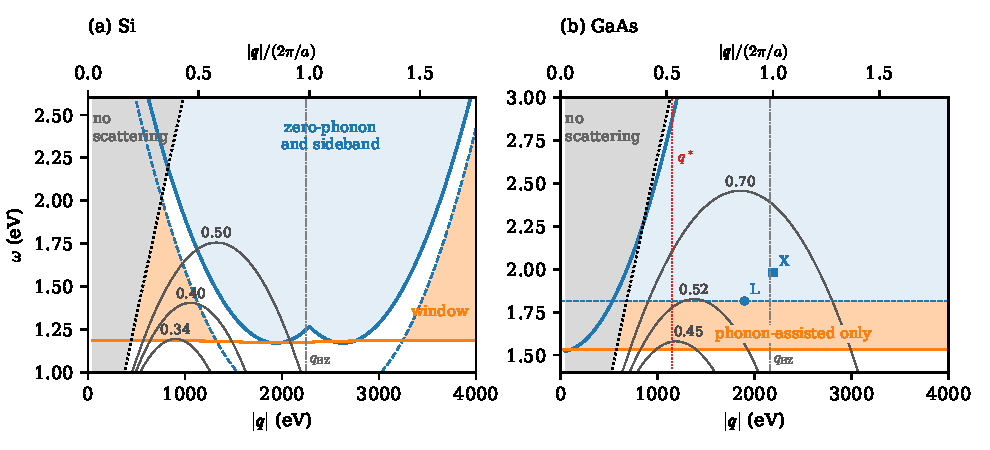
\includegraphics[width=\linewidth]{figures/ch17/fig17_4.pdf}
  \caption{Where the Migdal--phonon-assisted interference enters, in the plane of momentum transfer and energy deposited by scattering. (a)~Silicon. Thick blue: zero-phonon edge of the parabolic valleys along [100], $E_{\mathrm{min}} = \Eg + (q - K)^2/2M_{\mathrm{eh}}$ with $\Eg = \SI{1.17}{eV}$, $M_{\mathrm{eh}} = 1.193\,m_e$, $K = k_{\mathrm{c}} = 0.85\,(2\pi/a)$ and its images under $(2,0,0)\,2\pi/a$, a model that lies \SI{0.13}{eV} above the computed bands at \SI{1}{keV}. Dashed blue: the same lowered by the off-shell margin of the window, $\delta_w = \SI{0.3}{eV}$ (\cref{sec:8.6}). Orange line: the phonon-assisted threshold $\Eg + \omega_{\mathrm{TA}}(k_{\mathrm{c}} - q)$. Orange: the window, where the phonon-dressed sector is the only electronic final state and the cross term of \cref{eq:17.4-Sek} is a fraction of the whole electronic rate. White strip: the edge shell within $\delta_w$ of the zero-phonon edge, where only the sum of the two electronic sectors is defined. Light blue: zero-phonon pairs, with the phonon-dressed sector and its cross term a correction. (b)~GaAs: edge of the $\mathrm{\Gamma}$ pair with the [111] heavy hole ($\Eg = \SI{1.52}{eV}$, $M_{\mathrm{eh}} = 0.960\,m_e$), the L and X valleys at 1.815 and \SI{1.981}{eV} (points at $|\mathrm{\Gamma L}|$ and $|\mathrm{\Gamma X}|$), and the phonon-assisted threshold with the upper value \SI{10.5}{meV} of the transverse acoustic branch. Orange: below both the $\mathrm{\Gamma}$ edge and the L energy, phonon-assisted pairs only; the L valleys reach the line $\omega = \SI{1.815}{eV}$ near $|\mathrm{\Gamma L}|$ only. Red dotted: $q^* = \SI{1.15}{keV}$ of the GaAs window. Both panels: the largest deposit $qv_{\mathrm{max}} - q^2/2\mchi$ for the masses marked in MeV (gray), the envelope $qv_{\mathrm{max}}$ (dotted; gray region unreachable by scattering), and $q_{\mathrm{BZ}}$, the radius of the sphere with the volume of the zone (dash-dotted). Top axes: $q$ in units of $2\pi/a$; \cref{eq:17.4-lock} holds for $q \ll q_{\mathrm{BZ}}$.}
  \label{fig:17-interference}
\end{figure}

\Cref{fig:17-interference} places the cross term in the plane of $q$ and $\omega$. It exists wherever a pair with one phonon is kinematically allowed, above the phonon-assisted threshold, but it changes an observable rate by more than a correction to a correction in the window alone. There the phonon-dressed sector is the whole electronic rate of silicon between 0.3374 and \SI{0.405}{MeV} (\cref{tab:13-window}), and of GaAs from \SI{0.433}{MeV} to the opening of the L valleys at 0.52 to \SI{0.56}{MeV} (\cref{sec:13.1}).

\begin{workedexample}{The cross terms of a heavy dark photon in GaAs}\label{we:17-gaas-interference}
Take a dark photon with a heavy mediator, $\FDM = 1$, so that $\tilde V_e = \tilde V$ and $\tilde V_\kappa = -Z_\kappa\tilde V$ with $\tilde V$ independent of $q$, scattering in GaAs at $T = 0$. In the window it makes pairs only with a phonon, at momentum transfers near $q^* = \SI{1.15}{keV}$, 0.52 of $2\pi/a = \SI{2.193}{keV}$ (\cref{fig:17-interference}b).

\emph{Electron-following cell.} With $|Z^*| = 2.11$ (\cref{sec:5.5}), a gallium nucleus carries $Z = 31$ and its cloud $F^{\mathrm{fol}} = 28.89$ at long wavelength; an arsenic nucleus $Z = 33$ and $F^{\mathrm{fol}} = 35.11$. The separate terms are $961 + 834.6$ and $1089 + 1232.7$, the cross terms $-1791.2$ and $-2317.3$, and each total is $Z^{*2} = 4.452$: the cross term removes \SI{99.75}{\percent} and \SI{99.81}{\percent} of the two separate terms. The optical phonons that the dark photon makes are those of \cref{sec:11.2}. Without the cross cell their rate would be $(Z^2 + (F^{\mathrm{fol}})^2)/Z^{*2} = 403$ times (gallium) and 521 times (arsenic) larger, and the bare nuclear charges alone would give 216 and 245 times more, before the screening by $\varepsilon_\infty$ that both cases share.

\emph{Zero-phonon cell.} Above the opening of the L valleys the zero-phonon rate gains $2m_e\bar z$ from the ionic correction. The two values of $Z/M$, 0.4446 per u for gallium and 0.4405 per u for arsenic, differ by \SI{0.9}{\percent}. With $m_e = 5.486\times10^{-4}$\,u the cross cell is $4.88\times10^{-4}$ for weight on gallium alone and $4.83\times10^{-4}$ for weight on arsenic alone, and lies between the two for any positive weights. The zero-phonon Migdal cell is $(m_e\bar z)^2 = 5.9\times10^{-8}$.

\emph{Phonon-dressed cell.} In the window the whole electronic rate is phonon-assisted, and at leading order in $q$, \cref{eq:17.4-rate} with the mass-weighted mean gives it the same fraction, $4.8$ to $4.9\times10^{-4}$, and the one-phonon Migdal rate $5.9\times10^{-8}$ of it. Since $\mathfrak{D}$ has no $q$ dependence for a heavy mediator, the fraction is the same at every momentum transfer at this order, and the integrated rate carries it unchanged. At $q^*$, however, $q/(2\pi/a) = 0.52$, and the remainder of \cref{eq:17.4-lock} is not small. The cross term is of order $5\times10^{-4}$ of the phonon-assisted rate, with an uncertainty of order one in that fraction.

\emph{Screening.} The dark photon couples to the total charge, and both rows share the screening $1/\varepsilon$ of the total-charge row (\cref{sec:8.4}), which cancels from every fraction above.

\emph{Verdict.} The phonon-assisted rate of the silicon window is an estimate known to a factor of ten (\cref{tab:13-window}), and the GaAs window is known through its edges (\cref{sec:13.1}). The two electronic cross terms lie more than three orders of magnitude below such uncertainties. For a dark photon in GaAs the electron-following cell is the one that matters, and it decides the phonon rate.
\end{workedexample}

At small $q$ the nuclear amplitude in the electronic sectors is $(m_e/M_\kappa)\tilde V_{\mathrm{nuc}}/\tilde V_e$ times the electron amplitude. The cross term competes with the electron term when the coupling to a nucleus exceeds that to an electron by $M_\kappa/m_e = 5.1\times10^4$ in silicon, or, per nucleon, by $m_{\mathrm{u}}/m_e = 1823$. A scalar mixed with the Higgs boson, whose couplings follow the masses up to the nucleon matrix element, comes close to this; a $B - L$ vector, with couplings of equal size per nucleon and per electron, is far from it. For such a mediator a Migdal rate and an electron-recoil rate computed separately and added miss the true rate by the full cross term.

\section{Figures of merit per channel}\label{sec:17.5}

The heavy-mediator plateau of single-phonon emission is 1101 events per kilogram and year in germanium and 654 in silicon at $\sigma_p = 10^{-40}\,\mathrm{cm^2}$ (\cref{sec:11.1}). The ratio, 1.68, is the ratio of two sound speeds, and once the elastic tensors are known no phonon calculation is needed to obtain it. A number of this kind, a property of the material alone that the rate or the reach of one channel is proportional to, is what a comparison of targets needs. Such numbers exist for most channels of \cref{chap:10,chap:11,chap:12}, but each holds over a window of masses, and outside it the ratio of two rates is not the ratio of the two numbers. We will derive one such number per channel, with its window and inputs.

\subsection{Rate and reach figures of merit}\label{sec:17.5-def}

A figure of merit is either a reach number or a rate number. A \emph{reach figure of merit} is the lightest mass a channel can see, set by kinematics and one material energy or speed: the gap floor $2\Eg/v_{\mathrm{max}}^2$ of electronic excitations (\cref{eq:1.3-mmin}), the acoustic edge \cref{eq:11.1-edge}, the polar edge $2\omega_{\mathrm{L}}/v_{\mathrm{max}}^2$. These are exact statements about where a rate starts, and they rank materials without a window. A \emph{rate figure of merit} $F_A$ of material $A$ is a number that makes the rate per unit target mass factorize at fixed dark-matter parameters, $\mathcal{R}_A(\mchi) = G(\mchi)\,F_A$, with $G$ the same for every material. No real rate factorizes exactly, and the useful statement is about pairs. For two materials $A$ and $B$ we write
\begin{equation}
  \frac{\mathcal{R}_A(\mchi)}{\mathcal{R}_B(\mchi)} = \frac{F_A}{F_B}\,\bigl[1 + \delta_{AB}(\mchi)\bigr] ,
  \qquad
  W_{AB} = \bigl\{\mchi : |\delta_{AB}(\mchi)| < 0.1\bigr\} ,
  \label{eq:17.5-window}
\end{equation}
and call the contiguous range $W_{AB}$ the \emph{pairwise window} of the figure of merit, the masses at which the ratio of the two figures of merit gives the ratio of the rates to \SI{10}{\percent}. The tolerance is a convention, chosen to match the accuracy of most inputs. A window belongs to a pair, not to a material, because the corrections $\delta$ of two materials partly cancel when their properties are close and add when they are not. Several materials have a common window only if every pair among them has one, and \cref{sec:17.5-phonon} shows that this fails for sound speeds. \Cref{tab:17-fom} collects the figures of merit of every channel with their windows and the provenance of their inputs.

\begin{table}[tbp]
\centering
\caption{Figures of merit per channel, with the masses at which they rank two materials and the provenance of their inputs. Rates per unit target mass; $\omega_{\mathrm{th}} = \SI{1}{meV}$ for the phonon channels; standard halo of \cref{sec:1.2}. ``Pairwise'' refers to the window \cref{eq:17.5-window}. The absorption figures of merit are exact at each mass, since absorption fixes both $q$ and $\omega$.}
\label{tab:17-fom}
\footnotesize
\begin{tabular}{>{\raggedright\arraybackslash}p{0.13\linewidth}>{\raggedright\arraybackslash}p{0.19\linewidth}>{\raggedright\arraybackslash}p{0.27\linewidth}>{\raggedright\arraybackslash}p{0.16\linewidth}>{\raggedright\arraybackslash}p{0.09\linewidth}}
\toprule
Channel & Figure of merit & Where it ranks & Inputs & Silicon \\
\midrule
Electronic, reach & $2\Eg/v_{\mathrm{max}}^2$ & exact & $\Eg(T)$, measured & \SI{0.333}{MeV} \\
Electronic, rate & $L(q,\omega)$ in the window; ceiling $\propto Z_{\mathrm{val}}/A_{\mathrm{cell}}$ & no scalar ranks rates; ceiling with $\omega_p^{\mathrm{val}}$ for $qv_{\mathrm{max}} < \omega_{\mathrm{core}}$ (\cref{eq:17.5-partial}) & $L$ computed; $\nd_{\mathrm{val}}$, $\omega_p^{\mathrm{val}}$ measured & 0.142 \\
Acoustic, reach & $m_{\mathrm{min}}^{\mathrm{ac}}$ at $c_{\mathrm{LA,max}}$, \cref{eq:11.1-edge} & exact & $C_{ij}$, $\rho_T$ & \SI{6.1}{keV} \\
Acoustic, heavy mediator & $1/c_{\mathrm{NR1}}$, \cref{eq:17.5-cNR1} & pairwise: from about 4 edges of the softer crystal to the smaller $q_{\mathrm{BZ}}/2v_{\mathrm{max}}$; empty if speeds differ by $\gtrsim\SI{13.5}{km/s}$ & $C_{ij}$ measured or computed & 8.956\,km/s \\
Acoustic, light mediator & none (target independent) & equal rates above 44 times the higher edge & edge only & -- \\
Polar, rate & $\mathcal{I}_{\mathrm{pol}}/\rho_T$ with $\bar\omega_{\mathrm{pol}}$ & with $K_\eta(\bar\omega_{\mathrm{pol}},\mchi)$ at each mass; $\mathcal{I}_{\mathrm{pol}}/\rho_T$ alone only where the $K_\eta$ agree (LiF/GaAs above \SI{52}{MeV}) & $\varepsilon_\infty$, $\varepsilon_0$, $\omega_{\mathrm{T}\nu}$, $\omega_{\mathrm{L}\nu}$ measured, or $Z^*$ computed & -- \\
Polar, reach & $2\omega_{\mathrm{L}\nu}/v_{\mathrm{max}}^2$, lowest weighted branch & exact & $\omega_{\mathrm{L}\nu}$, measured & -- \\
Migdal & $F_{\mathrm{Mig}}$; pole limit \cref{eq:17.5-pole} & impulse regime (Si above \SI{17.5}{MeV}); ranking open & $L(p,\omega)$, $Z_{\mathrm{ion}}(p)$ computed & pole: 0.570, \SI{16.6}{eV} \\
Absorption & $L(0,m_\phi)/\rho_T$, $m_\phi\sigma_1/\rho_T$, scalar response per mass (\cref{sec:17.2}) & exact at each mass & optical data or computed & \cref{sec:17.2} \\
\bottomrule
\end{tabular}
\end{table}

\subsection{Gap floor and valence f-sum}\label{sec:17.5-electronic}

An electronic excitation needs at least $\Eg$, and the dark matter can deposit at most $\frac12\mchi v_{\mathrm{max}}^2$ (\cref{eq:1.3-omegamax}). The floor $2\Eg/v_{\mathrm{max}}^2$ is \SI{0.333}{MeV} for silicon with its physical gap of \SI{1.17}{eV}, \SI{0.212}{MeV} for germanium (\SI{0.744}{eV}) and \SI{0.433}{MeV} for GaAs (\SI{1.52}{eV}); with the step-model gap of \SI{1.11}{eV} that accompanies the silicon tables (\cref{sec:10.10}), it is \SI{0.316}{MeV}. Near the floor the rate is set by the spectrum within a few phonon energies of the edge. The gap is a measured input, and it must be the gap at the operating temperature of the detector, since the floor moves by the same fraction as the gap.

A rate figure of merit is harder. The electron-recoil rate weights the loss function over the window $\omega \le qv_{\mathrm{max}}$ by the halo factor. \Cref{we:10-fsum} showed that silicon puts a tiny part of its $f$-sum where a \SI{1}{MeV} particle can reach it: the computed rate is $4\times10^6$ times below the all-electron ceiling. Since the weight of the loss function inside the window varies between materials by orders of magnitude, no single number ranks electron-recoil rates; the loss function in the window is the figure of merit itself. What a single number can give is the ceiling. For it to be useful, the ceiling must count the electrons that absorb in the window and no others, and that needs a partial $f$-sum.

Split the dielectric function of an insulator with clamped nuclei into the contributions of the valence electrons and of the core,
\begin{equation*}
  \varepsilon(\omega) = \varepsilon_{\mathrm{val}}(\omega) + \varepsilon_{\mathrm{core}}(\omega) - 1 ,
\end{equation*}
each of them one plus the polarization of its group, at $q \to 0$. Three conditions make the valence part separable. (i) The two groups add, so that each obeys its own $f$-sum, $\int_0^\infty\dd\omega\,\omega\,\Imag\varepsilon_{\mathrm{val}} = (\pi/2)(\omega_p^{\mathrm{val}})^2$ with $(\omega_p^{\mathrm{val}})^2 = e^2\nd_{\mathrm{val}}/m_e$; this neglects the transfer of oscillator strength between shells that the Pauli principle causes (\cref{we:4-sifsum}). (ii) The valence absorption ends below the first core edge $\omega_{\mathrm{core}}$, and the core does not absorb below it. (iii) Over the valence spectrum the core part is real and equal to its static value, $\varepsilon_{\mathrm{core}}(\omega) \simeq \varepsilon_{\mathrm{core}}(0)$, which holds to order $\omega^2/\omega_{\mathrm{core}}^2$. By the Kramers--Kronig relation at $\omega = 0$ (\cref{eq:C.5-KKeps}),
\begin{equation*}
  \varepsilon_{\mathrm{core}}(0) - 1 = \frac{2}{\pi}\int_{\omega_{\mathrm{core}}}^\infty\dd\omega\,\frac{\Imag\varepsilon_{\mathrm{core}}(\omega)}{\omega} .
\end{equation*}
Below $\omega_{\mathrm{core}}$ we then have $\varepsilon = \varepsilon_{\mathrm{core}}(0) + \varepsilon_{\mathrm{val}} - 1$. Consider the model function $\varepsilon_{\mathrm{m}}(\omega) = \varepsilon_{\mathrm{core}}(0) + \varepsilon_{\mathrm{val}}(\omega) - 1$ at all frequencies, which equals $\varepsilon$ below the core edge to order $\omega^2/\omega_{\mathrm{core}}^2$. Above the valence spectrum $\varepsilon_{\mathrm{val}} - 1 \to -(\omega_p^{\mathrm{val}})^2/\omega^2$, so the function $g(\omega) = \varepsilon_{\mathrm{m}}^{-1}(\omega) - 1/\varepsilon_{\mathrm{core}}(0)$ falls as $(\omega_p^{\mathrm{val}})^2/[\varepsilon_{\mathrm{core}}(0)^2\omega^2]$. It is analytic in the upper half plane, being the inverse of a causal response with a constant subtracted, and the argument that turns the large-frequency tail of $\varepsilon^{-1}$ into the $f$-sum of the loss function (\cref{eq:4.4-fsumL}, \cref{app:C.5}) applies to it. For the true $\varepsilon$ the same tail is an intermediate asymptote, valid between the valence spectrum and the core edge, since at $\omega \to \infty$ the true $g$ tends to $1 - 1/\varepsilon_{\mathrm{core}}(0)$. Since $\Imag[-g] = L$ below $\omega_{\mathrm{core}}$, the loss function collected up to a cutoff $\omega_c$ between the valence spectrum and the core edge is
\begin{keyresult}[Partial (valence) f-sum of the loss function]
\begin{equation}
  \int_0^{\omega_c}\dd\omega\;\omega\,L(\omega) = \frac{\pi}{2}\,\frac{(\omega_p^{\mathrm{val}})^2}{\varepsilon_{\mathrm{core}}(0)^2} \simeq \frac{\pi}{2}\,(\omega_p^{\mathrm{val}})^2 ,
  \label{eq:17.5-partial}
\end{equation}
with $\omega_p^{\mathrm{val}}$ the plasma frequency of the valence electrons alone.
\end{keyresult}
\noindent The core screens the valence plasmon and lowers its weight by $\varepsilon_{\mathrm{core}}(0)^{-2}$. The absorption $\Imag\varepsilon$ collected over the same range carries no such factor, because $\varepsilon$ adds where $\varepsilon^{-1}$ does not. For silicon, $\nd_{\mathrm{val}} = \SI{2.00e23}{cm^{-3}}$ gives $\omega_p^{\mathrm{val}} = \SI{16.6}{eV}$ (\cref{we:4-siplasmon}), the measured plasmon energy, $16.6 \pm \SI{0.1}{eV}$ by electron energy loss~\cite[Table~I]{ramanathan2020ionization}. The core term follows from the photoabsorption above the L edge at \SI{99.8}{eV}: $\varepsilon_{\mathrm{core}}(0) - 1 = 0.0154$, so the core lowers the valence weight of $L$ by the factor $0.970$. A valence-only calculation, such as the tables of \cref{sec:10.2}, has no core and satisfies \cref{eq:17.5-partial} with $\varepsilon_{\mathrm{core}} = 1$; this is why \SI{16.6}{eV} is the right normalization of those tables (\cref{we:12-fsum}).

\begin{limitbox}[Partial f-sum of the valence electrons][lim:17.5a]
Below the first core edge the valence electrons carry the $f$-sum of the loss function $\int_0^{\omega_c}\omega L\,\dd\omega = (\pi/2)(\omega_p^{\mathrm{val}})^2$, with $\omega_p^{\mathrm{val}} = \SI{16.6}{eV}$ for silicon, the measured plasmon energy~\cite[Table~I]{ramanathan2020ionization}.
\par\smallskip
{\centering
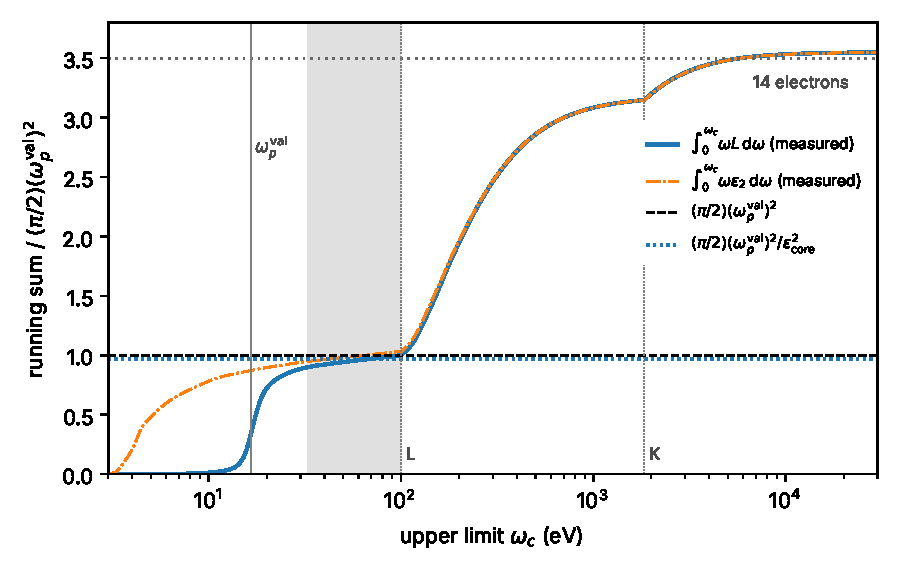
\includegraphics[width=\linewidth]{figures/ch17/limit17_5a.pdf}
\captionof{figure}{Running $f$-sums of silicon at $q \to 0$, $\int_0^{\omega_c}\omega L\,\dd\omega$ (solid) and $\int_0^{\omega_c}\omega\varepsilon_2\,\dd\omega$ (dash-dotted), in units of $(\pi/2)(\omega_p^{\mathrm{val}})^2 = \SI{433}{eV^2}$, against the upper limit $\omega_c$. Data: the measured optical constants of Franta and coworkers at \SI{300}{K} below \SI{35}{eV}~\cite{franta2017temperature} and the photoabsorption tables of Henke and coworkers above, with $\varepsilon = 1 - (\omega_a^2/\omega^2)(f_1 - \ii f_2)$, $\omega_a^2 = e^2\nd_{\mathrm{at}}/m_e$~\cite{henke1993xray}; moving the join to 30 or \SI{40}{eV} changes the $L$-sum below the L edge by \SI{0.8}{\percent}. Dashed: \cref{eq:17.5-partial} with $\varepsilon_{\mathrm{core}} = 1$; dotted: with the core term, 0.970. Vertical lines: $\omega_p^{\mathrm{val}}$ and the L and K edges at 99.8 and \SI{1839}{eV}; the dotted horizontal line at 3.5 is the sum of all 14 electrons per atom. Gray: $\omega_c$ from \SI{32.7}{eV} to the L edge, where the $L$-sum lies within \SI{10}{\percent} of the formula; just below the edge it is 1.000.}\label{fig:17-limit-a}
\par}
\smallskip
Below about $2\omega_p^{\mathrm{val}}$ the plasmon is not yet collected, and above the L edge the core electrons add their own sum, which rises toward 3.5 times the valence value.
\end{limitbox}

Just below the edge the measured $L$-sum is 1.000 of $(\pi/2)(\omega_p^{\mathrm{val}})^2$ and the $\varepsilon_2$-sum 1.032. The two corrections to \cref{eq:17.5-partial} are of similar size and opposite sign. The core screening lowers the $L$-sum by \SI{3}{\percent}, and the valence region holds \SI{3}{\percent} more absorption than four electrons, the strength moved up from the blocked core transitions. The data fix each of them to \SI{1.4}{\percent}, the amount by which the two sets together overshoot the all-electron sum of 14. The approach to the plateau is slow, because the plasmon at \SI{16.4}{eV} is broad: the $L$-sum reaches 0.9 at \SI{32.7}{eV}.

The partial sum turns the valence plasma frequency into a usable ceiling. \Cref{we:10-fsum} found that $\omega_p^{\mathrm{val}}$ in place of the all-electron \SI{31.1}{eV} does not give a bound, since the core electrons hold the rest of the $f$-sum. When the window lies entirely below the core edge, however, the energy integral of the bound runs over the valence spectrum alone, and by \cref{eq:17.5-partial} its weight is $(\pi/2)(\omega_p^{\mathrm{val}})^2$ to the few-percent accuracy of the two corrections; at finite $q$ the condition is $qv_{\mathrm{max}} < \omega_{\mathrm{core}}$. This is not a theorem, since the corrections need not stay small at finite $q$, but it lowers the ceiling of silicon by $(31.1/16.6)^2 = 3.5$ for every mass whose largest deposit, $\frac12\mchi v_{\mathrm{max}}^2$, lies below the L edge, $\mchi < \SI{28.4}{MeV}$. Per unit target mass the ceiling is proportional to $(\omega_p^{\mathrm{val}})^2/\rho_T = e^2Z_{\mathrm{val}}/(m_em_uA_{\mathrm{cell}})$, with $Z_{\mathrm{val}}$ valence electrons in a cell of $A_{\mathrm{cell}}$ mass units: the number of valence electrons per nucleon, 0.142 for silicon, 0.055 for germanium, 0.333 for diamond and 0.308 for LiF. This orders the ceilings, not the rates, which differ from them by the factor $10^{6}$ of \cref{we:10-fsum}.

\subsection{Acoustic edge and effective sound speed}\label{sec:17.5-phonon}

The one-phonon rate of \cref{eq:11.1-rate} has three figures of merit, one for each limit of the mediator and one for the edge. The reach figure of merit is the acoustic edge \cref{eq:11.1-edge}, evaluated at the fastest longitudinal speed $c_{\mathrm{LA,max}}$: \SI{6.1}{keV} for silicon, \SI{10.2}{keV} for germanium and \SI{3.1}{keV} for diamond at $\omega_{\mathrm{th}} = \SI{1}{meV}$. It is exact kinematics and ranks without a window. A stiff crystal reaches lower masses.

For a light mediator there is no rate figure of merit. The rate per unit mass tends to the target-independent value \cref{eq:11.1-light}, and the material enters through the correction factor $1 - (1 + \kappa_\eta)\,m_{\mathrm{min}}^{\mathrm{ac}}/\mchi$ alone, with the constant $\kappa_\eta$ of \cref{eq:11.1-correction}. Two materials have equal rates within \SI{10}{\percent} above 44 times the higher of their two edges (\cref{lim:11.1b}), and below that the edge, a reach number, decides.

For a heavy mediator, \cref{eq:11.1-heavy} gives a plateau inversely proportional to the polarization-weighted mean of the inverse sound speeds. Its inverse is an effective sound speed of the one-phonon nuclear rate,
\begin{equation}
  c_{\mathrm{NR1}} = \Bigl\langle\sum_\nu\frac{(\hat{\vect{q}}\cdot\hat{\vect{e}}_\nu)^2}{c_\nu(\hat{\vect{q}})}\Bigr\rangle_{\hat{\vect{q}}}^{-1} ,
  \qquad
  \mathcal{R} = \frac{2\rho_\chi\,\sigma_p\,I_0}{m_u^2\,c_{\mathrm{NR1}}} ,
  \label{eq:17.5-cNR1}
\end{equation}
so that the figure of merit is $1/c_{\mathrm{NR1}}$. It is \SI{8.956}{km/s} for silicon, \SI{5.321}{km/s} for germanium and \SI{18.16}{km/s} for diamond, within one percent of the sphere-averaged longitudinal speeds (\cref{lim:11.1c}) for these weakly anisotropic crystals. The speeds and polarizations come from the Christoffel problem of the elastic tensor (\cref{eq:C.18-christoffel}). The tensor is measured from the speed of ultrasound or from light scattered by thermal sound waves, or computed by density-functional theory from finite strains or from perturbation theory with strain as the perturbation (\cref{app:E.4}); \cref{app:E.17} specifies the elastic constants needed for the candidate targets. The two figures of merit pull in opposite directions: a soft lattice gives a large heavy-mediator rate and a high edge.

\Cref{eq:17.5-cNR1} drops two things, and each sets one end of the window. At low mass the lower cut $u_- = \omega_{\mathrm{th}}/(2\mchi c_\nu)$ of the integral $\int u^2\eta(c_\nu + u)\,\dd u$ removes the slowest part of the halo integral. Since $u_- = (v_{\mathrm{max}} - c_\nu)\,m_{\mathrm{min}}^{\mathrm{ac}}/\mchi$, it is a function of the mass in units of the edge, and it closes the window from below at a few times the edge of the softer crystal. At high mass the momentum transfers reach the zone scale, \cref{eq:11.1-Sac} stops holding, and the window ends at $m_{\mathrm{hi}} = q_{\mathrm{BZ}}/2v_{\mathrm{max}}$ of the crystal with the smaller zone, \SI{0.42}{MeV} for silicon (\cref{sec:11.1}). Between the two ends the window would be complete if the plateau were exact. It is not, and the reason is the shift of the halo integral by the sound speed.

Far above the edge, the integral of one branch and direction is $8\mchi^3\int_0^{v_{\mathrm{max}} - c_\nu}\dd u\,u^2\eta(c_\nu + u)$. With $v = c_\nu + u$ it becomes $8\mchi^3\int_{c_\nu}^{v_{\mathrm{max}}}\dd v\,(v - c_\nu)^2\eta(v)$, and expanding the square,
\begin{equation*}
  \int_{c_\nu}^{v_{\mathrm{max}}}\dd v\,(v - c_\nu)^2\eta(v) = I_0 - 2c_\nu I_1 + c_\nu^2 + O(c_\nu^3) ,
  \qquad
  I_1 = \int_0^{v_{\mathrm{max}}}\dd v\,v\,\eta(v) ,
\end{equation*}
where $I_0$ is the plateau integral of \cref{sec:11.1}. The coefficient of $c_\nu^2$ is $\int_0^\infty\eta\,\dd v = 1$, the normalization of the velocity distribution, since $\eta$ is its integral of $f_\chi/v$ above $\vmin$. The integral from $0$ to $c_\nu$ is of third order. Each branch and direction carries the weight $(\hat{\vect{q}}\cdot\hat{\vect{e}}_\nu)^2/c_\nu$, so the term $-2c_\nu I_1$ contributes $-2I_1\langle\sum_\nu(\hat{\vect{q}}\cdot\hat{\vect{e}}_\nu)^2\rangle = -2I_1$ by completeness, independent of the crystal. The rate in units of the plateau is
\begin{equation}
  \frac{\mathcal{R}\,c_{\mathrm{NR1}}\,m_u^2}{2\rho_\chi\sigma_pI_0} = 1 - \frac{2I_1}{I_0}\,c_{\mathrm{NR1}} + O(c^2) ,
  \qquad
  \frac{2I_1}{I_0} = \frac{5.88}{v_{\mathrm{max}}} = \frac{1}{\SI{135}{km/s}} ,
  \label{eq:17.5-shift}
\end{equation}
for the standard halo of \cref{sec:1.2}, with $\eta$ evaluated at $\vmin = c_\nu + q/2\mchi$ as in \cref{eq:11.1-rate}. For silicon the bracket is 0.934 at first order and 0.935 at second, against the largest computed ratio 0.936; for diamond 0.866 and 0.872, against 0.874. This is why the plateau of \cref{sec:11.1} is never reached: the halo is not flat at the large speeds that a heavy mediator favors.

The shift is linear in the sound speed and does not cancel between materials. For two crystals in the middle of their window,
\begin{equation*}
  \frac{\mathcal{R}_A\,c_{\mathrm{NR1},A}}{\mathcal{R}_B\,c_{\mathrm{NR1},B}} \simeq 1 - \frac{c_{\mathrm{NR1},A} - c_{\mathrm{NR1},B}}{\SI{135}{km/s}} .
\end{equation*}
Roughly, the inverse speeds rank two crystals to \SI{10}{\percent} as long as their effective speeds differ by less than \SI{13.5}{km/s}, which diamond and germanium, \SI{12.8}{km/s} apart, barely meet. The deviations of several crystals from a common reference add linearly in their speeds, and two crystals that both agree with silicon to \SI{10}{\percent} can disagree with each other by up to twice that. \Cref{fig:17-window} shows the ratio for five pairs. Germanium against silicon enters the band at \SI{43}{keV} and settles at 1.027; diamond against silicon enters at \SI{25}{keV} and settles at 0.933; CsI, a soft cubic crystal discussed below, enters at \SI{97}{keV} and reaches 1.045 at its zone cap. Diamond against CsI, however, is inside the band from 87 to \SI{227}{keV} alone and leaves it below the cap, where both still agree with silicon. A window ``against silicon'' does not give the ranking of the materials among themselves, and every pair needs its own.

\begin{figure}[tbp]
  \centering
  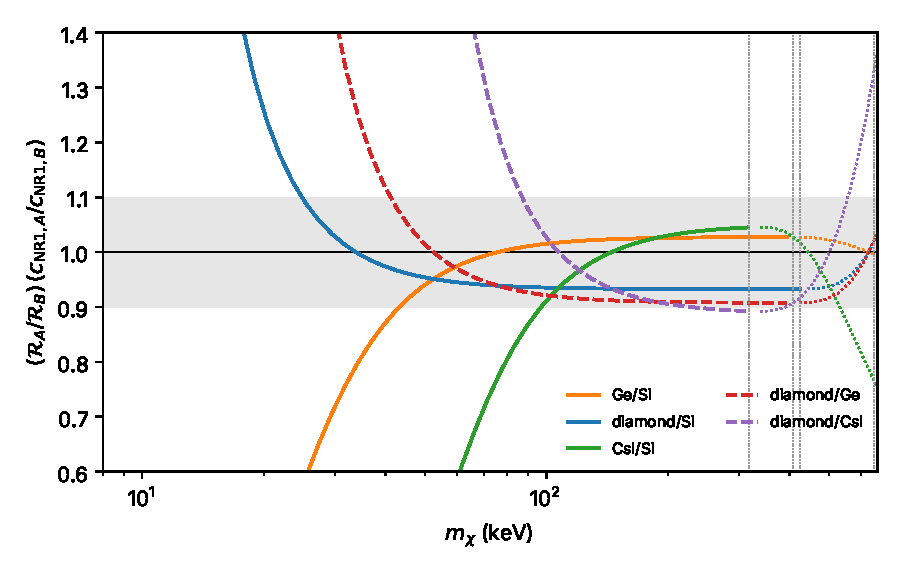
\includegraphics[width=0.85\linewidth]{figures/ch17/fig17_window.pdf}
  \caption{Heavy-mediator one-phonon rates of two crystals divided by the ratio of their figures of merit, $(\mathcal{R}_A/\mathcal{R}_B)(c_{\mathrm{NR1},A}/c_{\mathrm{NR1},B})$, against the dark-matter mass, from \cref{eq:11.1-rate} with all branches and directions, $q \le q_{\mathrm{BZ}}$, $\omega_{\mathrm{th}} = \SI{1}{meV}$, the orientation average and the standard halo of \cref{sec:1.2}. Elastic tensors: measured room-temperature values for Si, Ge and diamond (\cref{we:11-cbar}); CsI at \SI{4.2}{K}~\cite{vallin1964elastic} with the room-temperature density \SI{4.529}{g.cm^{-3}}. Gray: the \SI{10}{\percent} band of the pairwise window \cref{eq:17.5-window}. Each curve is solid up to the smaller $q_{\mathrm{BZ}}/2v_{\mathrm{max}}$ of its pair (vertical dotted lines: 0.32, 0.41, 0.42 and \SI{0.65}{MeV} for CsI, Ge, Si and diamond) and dotted above. At high mass the curves settle at $1 - (c_{\mathrm{NR1},A} - c_{\mathrm{NR1},B})/(\SI{135}{km/s})$, \cref{eq:17.5-shift}.}
  \label{fig:17-window}
\end{figure}

\begin{workedexample}{The pairwise window of diamond against silicon}\label{we:17-window}
Diamond has $c_{\mathrm{NR1}} = \SI{18.16}{km/s}$ and silicon \SI{8.956}{km/s}, so the figure of merit predicts a heavy-mediator rate ratio of $8.956/18.16 = 0.493$: the plateaus of \cref{eq:17.5-cNR1} are 322.6 and 654.0 events per kilogram and year at $\sigma_p = 10^{-40}\,\mathrm{cm^2}$ and $\omega_{\mathrm{th}} = \SI{1}{meV}$. The edges at the effective speeds are \SI{3.19}{keV} for diamond and \SI{6.39}{keV} for silicon, and the zone caps $q_{\mathrm{BZ}}/2v_{\mathrm{max}}$ are 0.65 and \SI{0.42}{MeV}, so the window can extend at most to \SI{0.42}{MeV}.

The full rates \cref{eq:11.1-rate} give the correction $1 + \delta$ of \cref{eq:17.5-window}, the rate ratio divided by 0.493:
\begin{center}
\small
\begin{tabular}{lccccccc}
\toprule
$\mchi$ (keV) & 10 & 20 & 30 & 45 & 100 & 300 & 420 \\
$\mathcal{R}_{\mathrm{Si}}$ & 66.0 & 432.5 & 546.7 & 590.6 & 609.8 & 612.0 & 612.2 \\
$\mathcal{R}_{\mathrm{C}}$ & 199.3 & 268.0 & 277.3 & 280.2 & 281.4 & 281.6 & 281.7 \\
$1 + \delta$ & 6.12 & 1.256 & 1.028 & 0.962 & 0.935 & 0.933 & 0.933 \\
\bottomrule
\end{tabular}
\end{center}
with the rates in events per kilogram and year. At \SI{10}{keV} silicon is less than two edges above its threshold and diamond leads by a factor of three, against the predicted half. The lower cut explains it: at \SI{20}{keV} it removes the halo below $u_- = \SI{251}{km/s}$, $0.32\,v_{\mathrm{max}}$, for silicon, but only below \SI{124}{km/s} for diamond, whose phonons of \SI{1}{meV} carry half the momentum. The ratio crosses 1.1 at \SI{24.8}{keV}, 3.9 times the edge of silicon, and the window opens there.

Above \SI{100}{keV} the correction no longer depends on the mass. It is the shift \cref{eq:17.5-shift}: to first order $1 - (18.16 - 8.956)/135 = 0.932$, and with the exact single-speed integrals $\int_c^{v_{\mathrm{max}}}(v - c)^2\eta\,\dd v/I_0$, 0.8724 for diamond and 0.9354 for silicon, the ratio is 0.9327, the computed value to four digits. The window is
\begin{equation*}
  W_{\mathrm{C,Si}} = \SI{25}{keV}\text{ to }\SI{0.42}{MeV} ,
\end{equation*}
inside which $1 + \delta$ runs from 1.088 down to 0.933. The figure of merit ranks the pair correctly above \SI{14}{keV}, 2.2 times the edge of silicon, where the two rates cross; below that the cut of the softer crystal reverses the order. Inside $W_{\mathrm{C,Si}}$ it also gives the ratio to \SI{10}{\percent}, but even there it is biased by \SI{7}{\percent} against the stiffer crystal. Against germanium, \SI{12.8}{km/s} softer, diamond settles at 0.908, at the edge of the band.
\end{workedexample}

Tabulated sound speeds feed most published comparisons of targets, and they can be tested against measured elasticity without any phonon calculation. For a cubic crystal the floor \cref{eq:11.1-rayleigh}, $c_{\mathrm{LA}} \ge \sqrt{B/\rho_T}$, needs the bulk modulus alone; for any crystal the Christoffel problem of a measured tensor gives the range of longitudinal speeds over all directions. The target table of Griffin and collaborators lists one longitudinal speed per material, a sphere average of $\omega_{\mathrm{LA}}/q$ from density-functional phonons~\cite[Table~I and App.~A\,3]{griffin2020multichannel}. \Cref{tab:17-speeds} tests five of its entries against measured tensors, and all five fail.

\begin{table}[tbp]
  \caption{Tabulated longitudinal sound speeds~\cite[Table~I]{griffin2020multichannel} against measured elastic constants (GPa). Hexagonal crystals: $C_{11}$, $C_{12}$, $C_{13}$, $C_{33}$, $C_{44}$, the recommended values of Vurgaftman and Meyer for the nitrides as quoted in~\cite[Table~I]{lopuszynski2012composition}, and the Brillouin values for ZnO as quoted in~\cite[Table~III]{gopal2006polarization}. CsI (cubic, \SI{4.2}{K}): $C_{11}$, $C_{12}$, $C_{44}$~\cite[abstract]{vallin1964elastic}. CaWO$_4$ (tetragonal, point group $4/m$, which allows $C_{16} = -C_{26}$): ultrasonic data of Farley and Saunders~\cite{farley1972ultrasonic} as quoted in~\cite[p.~16]{popova2025high}. Densities from the measured lattice constants (CsI at room temperature). Range: the longitudinal speeds of the Christoffel problem over all directions.}
  \label{tab:17-speeds}
  \centering\footnotesize\setlength{\tabcolsep}{3pt}
  \begin{tabular}{@{}l>{\raggedright\arraybackslash}p{0.29\linewidth}cccc@{}}
    \toprule
    Crystal & Measured constants & $\rho_T$ (\si{g.cm^{-3}}) & Range (\si{km/s}) & Tabulated (\si{km/s}) & Tabulated/range \\
    \midrule
    GaN & 390, 145, 106, 398, 105 & 6.09 & 7.64--8.08 & 12.50 & 1.55 of max \\
    AlN & 396, 137, 108, 373, 116 & 3.26 & 10.52--11.02 & 17.09 & 1.55 of max \\
    ZnO & 206, 118, 118, 211, 44 & 5.67 & 6.03--6.10 & 12.53 & 2.05 of max \\
    CsI & 27.37, 7.93, 8.25 & 4.529 & 2.37--2.46 & 1.379 & 0.58 of min \\
    CaWO$_4$ & $C_{11} = 145.9$, $C_{33} = 127.4$, $C_{12} = 62.6$, $C_{13} = 39.2$, $C_{16} = -19.2$, $C_{44} = 33.5$, $C_{66} = 38.7$ & 6.115 & 4.36--5.17 & 4.257 & 0.98 of min \\
    \bottomrule
  \end{tabular}
\end{table}

The nitrides and ZnO are listed above every longitudinal speed of their measured tensors; the older handbook constants of the nitrides give the ratios 1.59 and 1.52 instead of 1.55. CsI is listed below them: its room-temperature bulk modulus, \SI{13.5}{GPa}~\cite[Table~I]{buongiornonardelli1995high}, puts the floor at \SI{1.726}{km/s}, \SI{25}{\percent} above the tabulated value, and the tabulated speed is \SI{42}{\percent} below the slowest direction of the measured tensor. CaWO$_4$ is listed \SI{8.4}{\percent} below its sphere average, \SI{4.65}{km/s}, and below its slowest direction. For silicon the same table is \SI{5.6}{\percent} below the measured average (\cref{we:11-cbar}). The errors matter for the figures of merit. With its measured tensor CsI has $c_{\mathrm{NR1}} = \SI{2.40}{km/s}$ and a heavy-mediator figure of merit 3.73 times that of silicon, against 6.49 from the tabulated speed; its acoustic edge, from $c_{\mathrm{LA,max}} = \SI{2.46}{km/s}$, is \SI{23.1}{keV}. CaWO$_4$ has $c_{\mathrm{NR1}} = \SI{4.58}{km/s}$, 1.96 times silicon against 2.10, and an edge of \SI{11.0}{keV}.

\subsection{Polar band integral and polar edge}\label{sec:17.5-polar}

For a light dark photon the single-phonon rate of a polar crystal is the band integral $\mathcal{I}_{\mathrm{pol}}$ of the loss function, each line weighted by the kinematic factor $K_\eta(\omega,\mchi)$ of \cref{eq:11.2-rate}. \Cref{sec:11.2} takes $K_\eta$ at the weighted mean frequency $\bar\omega_{\mathrm{pol}}$, which makes $\mathcal{I}_{\mathrm{pol}}/\rho_T$ of \cref{we:11-ipol} the natural figure of merit. It factorizes only if $K_\eta$ is the same for both crystals, and it is not, because $K_\eta$ depends on the frequency. For a single speed $K_\eta = \ln(q_+/q_-)/v$ (\cref{sec:11.2-rate}), and far above the edge $\ln(q_+/q_-) \simeq \ln(2\mchi v^2/\omega)$, so the ratio of the weights of two crystals approaches one only logarithmically:
\begin{equation*}
  \frac{K_\eta(\omega_A,\mchi)}{K_\eta(\omega_B,\mchi)} \simeq 1 - \frac{\ln(\omega_A/\omega_B)}{\ln(2\mchi v^2/\omega_B)} , \qquad v \simeq v_0 .
\end{equation*}
The halo average puts the effective speed in the logarithm near $v_0$. For LiF against GaAs, longitudinal energies of 77.2 and \SI{36.35}{meV}, this gives 0.79 at \SI{1}{MeV} and 0.87 at \SI{10}{MeV}, against the full weights 0.77 and 0.87, and it reaches 0.9 at \SI{54}{MeV} against the full \SI{52}{MeV}; at \SI{100}{keV} the full ratio is 0.34. Sapphire, with $\bar\omega_{\mathrm{pol}} = \SI{109.9}{meV}$, reaches the band at \SI{1.7}{GeV}. The pairwise window of $\mathcal{I}_{\mathrm{pol}}/\rho_T$ alone is thus empty below tens of MeV for crystals whose optical energies differ by a factor of two, which covers most pairs of interest. The figure of merit of the polar channel is a pair of numbers, $\mathcal{I}_{\mathrm{pol}}/\rho_T$ and $\bar\omega_{\mathrm{pol}}$, and the rate ratio at a given mass is $(\mathcal{I}_{\mathrm{pol},A}/\rho_{T,A})K_\eta(\bar\omega_{\mathrm{pol},A},\mchi)$ over the same for $B$. Its inputs, and their fragility on the dielectric route, are those of \cref{we:11-ipol,lim:11.2d}; a crystal known through $\varepsilon_\infty$, $\varepsilon_0$ and $\omega_{\mathrm{T}}$ alone is ranked by its interval.

The reach figure of merit is the polar edge, $2\omega_{\mathrm{L}\nu}/v_{\mathrm{max}}^2$ for the lowest longitudinal branch with weight: \SI{10.35}{keV} for GaAs, \SI{21.98}{keV} for LiF, and between 13.7 and \SI{32.0}{keV} for the four branches of sapphire. Rate and reach rank in opposite orders, since a high optical frequency raises the band integral, at fixed screening, density and ratio $\omega_{\mathrm{L}}/\omega_{\mathrm{T}}$, and raises the edge by the same factor; the reach curves of LiF and GaAs cross at \SI{26.7}{keV} (\cref{sec:11.2}).

\subsection{Migdal plasmon-pole factor}\label{sec:17.5-migdal}

In the per-mass Migdal rate \cref{eq:12.3-permass} the material enters as $\omega_e^{-4}\sum_\kappa N_\kappa L_{\mathrm{Mig},\kappa}/A_{\mathrm{cell}}$, with $N_\kappa$ atoms of species $\kappa$ in a cell of $A_{\mathrm{cell}}$ mass units and $L_{\mathrm{Mig},\kappa}$ the loss function seen by its ion. Above a threshold the figure of merit is its integral,
\begin{equation*}
  F_{\mathrm{Mig}} = \sum_\kappa\frac{N_\kappa}{A_{\mathrm{cell}}}\int_{\omega_{\mathrm{th}}}\dd\omega\;\frac{L_{\mathrm{Mig},\kappa}(\omega)}{\omega^4} ,
\end{equation*}
valid where \cref{eq:12.3-permass} is: in the impulse regime, above \SI{17.5}{MeV} for silicon (\cref{sec:11.4}), with the per-mass form within \SI{10}{\percent} of the exact free-recoil rate above \SI{66}{MeV} (\cref{lim:12.3c}), for $\mchi \ll M_\kappa$ and for deposits small against the kinetic energy of the dark matter. The floor is the electronic one, $2\Eg/v_{\mathrm{max}}^2$. $F_{\mathrm{Mig}}$ needs the loss function at the large momenta of the ion's field, mostly 3 to \SI{9}{keV} in silicon (\cref{sec:12.3}), and no tabulated quantity gives it. Two limits show what it depends on.

Suppose first that at every $p$ the valence loss function is a single plasmon pole carrying the partial $f$-sum \cref{eq:17.5-partial}, $L(p,\omega) = (\pi/2)[(\omega_p^{\mathrm{val}})^2/\omega_{\mathrm{pl}}(p)]\,\delta(\omega - \omega_{\mathrm{pl}}(p))$. Then $\int\dd\omega\,L/\omega^4 = (\pi/2)(\omega_p^{\mathrm{val}})^2/\omega_{\mathrm{pl}}(p)^5$, which tends to $(\pi/2)(\omega_p^{\mathrm{val}})^{-3}$ at small $p$, and with the small-$p$ ion charges
\begin{equation}
  F_{\mathrm{Mig}} \propto \sum_\kappa\frac{N_\kappa Z_{\mathrm{ion},\kappa}^2}{A_{\mathrm{cell}}}\,\frac{\pi}{2}\,(\omega_p^{\mathrm{val}})^{-3}
  \qquad\text{(plasmon pole)} .
  \label{eq:17.5-pole}
\end{equation}
The nuclear factor $\sum_\kappa N_\kappa Z_{\mathrm{ion},\kappa}^2/A_{\mathrm{cell}}$ favors light nuclei: 0.570 for silicon ($Z_{\mathrm{ion}} = 4$) and 1.928 for LiF ($Z_{\mathrm{ion}} = 1$ and 7 with the $1s$ shells in the cores), a factor 3.38. The pole factor gives it back. LiF has eight valence electrons per formula unit in a cubic cell of \SI{4.020}{\angstrom} holding four of them~\cite[Table~III]{griffin2020multichannel}, so $\omega_p^{\mathrm{val}} = \SI{26.1}{eV}$, and the pole factors stand in the ratio 3.87. In the pole limit LiF has 0.87 of the Migdal figure of merit of silicon. Note, however, that the valence count of LiF includes the shallow fluorine $2s$ shell, and that the lithium $1s$ edge lies not far above the valence spectrum, so condition (ii) of the partial $f$-sum holds there only marginally. Germanium, with $\omega_p^{\mathrm{val}} = \SI{15.6}{eV}$ and $Z_{\mathrm{ion}} = 4$ with the $3d$ shell in the core, has 0.47 of it. Its $3d$ shell is shallow and polarizable, so $\varepsilon_{\mathrm{core}}(0) - 1$ is far larger than the 0.0154 of silicon, and this factor carries an unsized error from the screening by the core and its hybridization with the valence bands.

\Cref{eq:17.5-pole} ignores the dispersion of the pole. The Migdal weight sits at $p$ of several keV, not at $p \to 0$, and with a dispersing pole the integral over $p$ depends on the material through $\omega_{\mathrm{pl}}(p)$. For a pole $\omega_{\mathrm{pl}}^2 = \omega_p^2 + (3/5)v_{\mathrm{F}}^2p^2$ integrated over all $p$, $\int p^2\dd p\,\omega_p^2/\omega_{\mathrm{pl}}^5 \propto v_{\mathrm{F}}^{-3} \propto (\omega_p^{\mathrm{val}})^{-2}$; for $\omega_{\mathrm{pl}}^2 = \omega_p^2 + (p^2/2m_e)^2$ it scales as $(\omega_p^{\mathrm{val}})^{-3/2}$. LiF then has 1.37 to 1.72 of the figure of merit of silicon instead of 0.87, and germanium 0.42 to 0.44. The pole limit is uncertain by a factor of two in its scaling between materials, and even the order of LiF and silicon depends on the dispersion.

The opposite limit puts the weight at the gap. For any loss function that starts at $\Eg$, the partial $f$-sum bounds $\int_{\Eg}\dd\omega\,L/\omega^4$ by $(\pi/2)(\omega_p^{\mathrm{val}})^2/\Eg^5$ at each $p$, the bound \cref{sec:12.3} states with the full plasma frequency. For silicon the bound exceeds the pole value by $(\omega_p^{\mathrm{val}}/\Eg)^5 = 5.7\times10^5$, and between silicon and LiF ($\Eg = \SI{14.2}{eV}$) it changes the order: the bound on the energy integral of silicon is $1.1\times10^5$ times that of LiF, and $3.2\times10^4$ times with the nuclear factor. Silicon is close to the gap end. Its computed spectrum puts \SI{4}{\percent} of the Migdal probability in the plasmon and half of it below \SI{4.6}{eV} (\cref{sec:12.3}), so the weight just above the gap, not the plasmon, sets its figure of merit. The pole scaling \cref{eq:17.5-pole} is a statement about crystals whose loss function is dominated by the plasmon at the momenta of the ion's field. Where real crystals sit between the two limits can be decided only with the computed $L(p,\omega)$ near the gap at momenta of several keV, with the valence split of $Z_{\mathrm{ion}}$ and $L$ made consistently. The ranking of Migdal targets that would follow is an open problem, which the guide to next targets at the end of the book takes up.

\section{Ranking under uncertainty}\label{sec:17.6}

Paratellurite, TeO$_2$, has the softest lattice of the crystals we rank: its effective sound speed $c_{\mathrm{NR1}}$, the inverse of its heavy-mediator figure of merit (\cref{sec:17.5}), is \SI{3.75}{km/s}, against \SI{4.58}{km/s} for CaWO$_4$ and \SI{8.96}{km/s} for silicon. Its single-phonon rate per unit mass should then be 2.39 times silicon's, and 1.22 times that of CaWO$_4$. The speeds of CaWO$_4$ and TeO$_2$ have different origins, however. The speed of CaWO$_4$ follows from an ultrasonic measurement of its elastic tensor; the speed of TeO$_2$ follows from a tensor computed with a density functional, whose errors are of order \SI{10}{\percent} and are not stated with the number. Whether TeO$_2$ beats CaWO$_4$ depends on those errors.

\subsection{Provenance widths}\label{sec:17.6-widths}

Every input of a figure of merit is one of three kinds. A \emph{measured} input comes from an experiment on the crystal: the low-temperature gap of silicon, \SI{1.17}{eV} (\cref{tab:3-materials}), or the elastic constants of germanium, 131, 49 and \SI{68}{GPa} (\cref{sec:11.1}). A \emph{computed} input comes from a first-principles calculation, such as the elastic tensors of a materials database or the Born charges of a density-functional perturbation calculation. An \emph{estimated} input is a parametric guess or a prior, such as the shift of a gap from room temperature to the millikelvin temperatures of a detector. We give each input a lognormal distribution, $\ln x_j$ Gaussian about $\ln x_{j0}$ with width $\sigma^{\mathrm{prov}}_j$, or a stated uniform prior. The provenance width $\sigma^{\mathrm{prov}}_j$ is a convention, set by the kind of input rather than worked out number by number; \cref{tab:17-widths} lists the values we use.

\begin{table}[tbp]
  \caption{Provenance widths: the Gaussian width $\sigma^{\mathrm{prov}}_j$ of $\ln x_j$, or the prior, assigned to each kind of input of a figure of merit. The values are conventions. The widths for computed sound speeds and for room-temperature gaps are tested against the book's crystals in \cref{sec:17.6-widths}; the prior on $X_{\mathrm{pole}}$ is a device (\cref{sec:17.6-correlation}).}
  \label{tab:17-widths}
  \centering\footnotesize\setlength{\tabcolsep}{4pt}
  \begin{tabular}{@{}>{\raggedright\arraybackslash}p{0.30\linewidth}>{\raggedright\arraybackslash}p{0.36\linewidth}>{\raggedright\arraybackslash}p{0.26\linewidth}@{}}
    \toprule
    Kind of input & Example & Width \\
    \midrule
    Measured, spread stated & sapphire $\mathcal{I}_{\mathrm{pol}}$ through $\varepsilon_\infty = 3.1$--3.3; GaAs $\mathcal{I}_{\mathrm{pol}}$, half the spread of its dielectric and splitting routes & 0.03; 0.04 \\
    Measured, no error stated & gap at low temperature; speed from a measured tensor; frequency of a measured phonon & 0.01; 0.02; 0.005 \\
    Measured at room temperature, used at low temperature & gap of a crystal without low-temperature data & room-temperature value plus a shift uniform on 0.03--\SI{0.10}{eV} \\
    Computed, materials database & sound speed from a computed elastic tensor; density of a computed cell & 0.086; 0.030 \\
    Computed, density-functional perturbation theory & Born charge $Z^*$, $\varepsilon_\infty$; optical-phonon energy & 0.07; 0.05 \\
    Estimated & interband enhancement $X_{\mathrm{pole}}$ of the Migdal pole factor & log-uniform on [1, 3] \\
    \bottomrule
  \end{tabular}
\end{table}

Two widths decide most of the rankings, and the book's own crystals test both. For computed sound speeds we take the elastic tensors of the JARVIS (Joint Automated Repository for Various Integrated Simulations) database, obtained with one exchange--correlation functional, OptB88vdW, for every crystal~\cite{choudhary2018elastic}. Silicon, germanium and diamond have measured tensors (\cref{sec:11.1}), so the database can be compared with experiment on the same quantity. Solving the Christoffel problem for the database and the measured tensors gives database values of $c_{\mathrm{NR1}}$ below the measured ones by \SI{2.9}{\percent} for silicon, \SI{10.2}{\percent} for germanium and \SI{1.0}{\percent} for diamond. The root mean square of the logarithmic differences is 0.065, inside the width 0.086 we assign. All three differences have the same sign, however, with a mean of $-0.048$: the errors of one method are not independent from crystal to crystal (\cref{sec:17.6-correlation}). For gaps, the shift from room temperature to low temperature is 0.05, 0.08 and \SI{0.10}{eV} for silicon, germanium and GaAs (\cref{tab:3-materials}); a crystal whose gap is known at room temperature alone gets a shift drawn uniformly between 0.03 and \SI{0.10}{eV}. Neither width is a bound: a crystal whose computed tensor errs by \SI{25}{\percent}, or whose gap moves by \SI{0.2}{eV} on cooling, is not excluded by the convention.

The halo enters every edge through the same power of $v_{\mathrm{max}}$, so a common factor on $v_{\mathrm{max}}$ multiplies all edges alike and changes no order in any draw. We keep $v_{\mathrm{max}} = 2.650\times10^{-3}$ fixed.

Our pool of crystals consists of silicon, germanium, GaAs and diamond, and seven insulators that cryogenic experiments use or propose: sapphire, LiF, NaF, CaWO$_4$, TeO$_2$, Li$_2$MoO$_4$ and $\gamma$-LiAlO$_2$. Each probability below is taken over this pool. The gaps of silicon, germanium and GaAs are the low-temperature values 1.17, 0.744 and \SI{1.52}{eV} of \cref{tab:3-materials}, and the gap of diamond, 5.47~eV, is a low-temperature value as well; sapphire (8.8~eV), CaWO$_4$ (5.2~eV), NaF (11.5~eV) and LiF (14.2~eV) enter with room-temperature gaps~\cite[Table~I]{griffin2020multichannel}. The tensors of silicon, germanium and diamond are the measured ones of \cref{sec:11.1}, and CaWO$_4$ enters with the measured tensor of \cref{sec:17.5-phonon}. GaAs, sapphire, TeO$_2$, $\gamma$-LiAlO$_2$, LiF and NaF enter with database tensors and the densities of their computed cells; Li$_2$MoO$_4$ has no tensor in the database and is not ranked in the two channels that need one, the heavy-mediator single-phonon rate and the nuclear edge. The polar inputs of GaAs and sapphire are those of \cref{sec:11.2}: $\mathcal{I}_{\mathrm{pol}}/\rho_T = 0.1415$ for GaAs (the splitting route of \cref{we:11-ipol}) and 9.12 for the ordinary axis of sapphire, both from measured frequencies. For LiF and NaF, \cref{eq:11.2-diatomic} gives 19.0 and $\SI{9.95}{meV.cm^3.g^{-1}}$ with the computed $Z^* = 1.05$ and 0.98, $\varepsilon_\infty = 2.02$ and 1.78, and highest optical energies 77.2 and \SI{49.9}{meV}~\cite[Table~I]{griffin2020multichannel}.

\subsection{Monte Carlo rank statistics}\label{sec:17.6-mc}

With every input a distribution, the figure of merit of each material is sampled by Monte Carlo as in \cref{app:C.14}: we draw $N_{\mathrm{MC}} = 2\times10^4$ sets of inputs, evaluate the figure of merit of every material on each set, and record the order in every draw.

\begin{keyresult}[Ranking under uncertainty]
For each material $A$ of a pool and each draw $k$ of the inputs, let $R_A^{(k)}$ be the rank of $A$ in that draw. Then
\begin{equation}
  P_A(\mathrm{first}) = \frac{1}{N_{\mathrm{MC}}}\sum_{k=1}^{N_{\mathrm{MC}}}\mathbb{1}\bigl[R_A^{(k)} = 1\bigr] , \qquad
  \text{rank interval} = \bigl[R_A^{16}, R_A^{84}\bigr] ,
  \label{eq:17.6-pfirst}
\end{equation}
where $R_A^{16}$ and $R_A^{84}$ are the 16th and 84th percentiles of $R_A^{(k)}$. The tier of $A$ is its height $h(A)$, \cref{eq:C.13-height}, in the interval order \cref{eq:C.13-order} of the 68\% intervals of the figure of merit. All three quantities are conditional on the provenance widths of \cref{tab:17-widths}.
\end{keyresult}

The probabilities $P_A(\mathrm{first})$ sum to one over the pool in every channel, and the sampling error of each is at most $[p(1 - p)/N_{\mathrm{MC}}]^{1/2} \le 0.0035$.

The probability of ranking first measures whether the widths can overturn a lead, not how large the lead is. TeO$_2$ leads the heavy-mediator channel with $P(\mathrm{first}) = 0.968$, and its 68\% interval of $c_{\mathrm{NR1}}(\mathrm{Si})/c_{\mathrm{NR1}}$ is $[2.19, 2.60]$; CaWO$_4$, measured, has the narrow interval $[1.92, 2.00]$ and $P(\mathrm{first}) = 0.010$. With the computed-speed width doubled to 0.172, TeO$_2$ falls to $P(\mathrm{first}) = 0.781$ and GaAs, also computed, rises from 0.022 to 0.135, while CaWO$_4$ gains just from 0.010 to 0.073.

The rank interval says where a material stands when it does not lead. Silicon, in the same channel, has the rank interval 8--8: it is eighth in at least 68\% of the draws, ahead only of sapphire and diamond, whose lattices are stiffer. CaWO$_4$ and GaAs share the interval 2--3. A rank interval that spans several places marks a material whose position the inputs do not fix; the interval says nothing about which neighbor the material trades places with.

\begin{figure}[tbp]
  \centering
  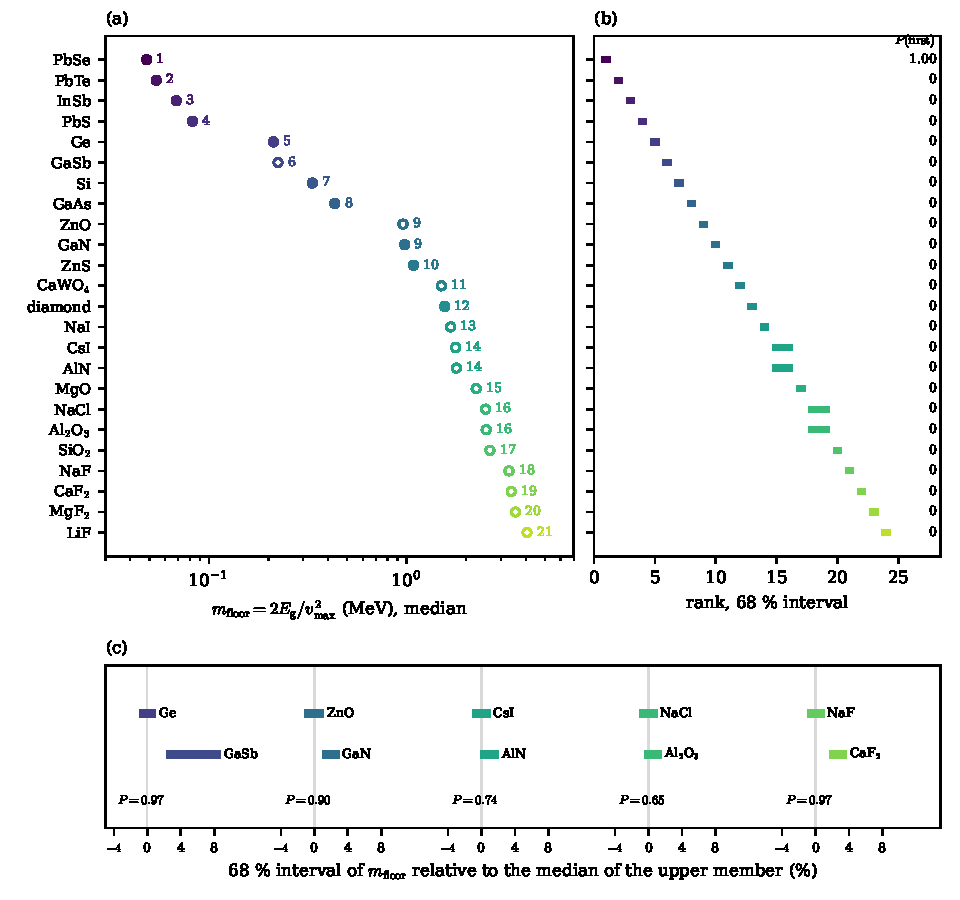
\includegraphics[width=\linewidth]{figures/ch17/fig17_5.pdf}
  \caption{Rank intervals for the electron-recoil floor $2\Eg/v_{\mathrm{max}}^2$, $v_{\mathrm{max}} = 2.650\times10^{-3}$, of the 24 crystals in the target table of Griffin and collaborators~\cite[Table~I]{griffin2020multichannel}, with the low-temperature gaps of \cref{tab:3-materials} for silicon, germanium and GaAs. (a)~Median floor; filled symbols: gap measured at low temperature, open symbols: room-temperature gap plus an upward shift drawn uniformly on 0.03--\SI{0.10}{eV}; gap width 0.01 in the logarithm for all. Numbers and colors: tier (height in the interval order of the 68\% intervals). (b)~Rank, 16th to 84th percentile over $2\times10^4$ draws, and the probability of ranking first. (c)~The 68\% intervals of five close pairs, relative to the median of the member with the lower floor, with the probability $P$ that this member has the lower floor. Pairs in one tier overlap; pairs in different tiers do not, whatever $P$.}
  \label{fig:17-rank-floor}
\end{figure}

\Cref{fig:17-rank-floor} shows the electron-recoil floor $2\Eg/v_{\mathrm{max}}^2$, the lightest mass at which dark matter can cross the gap (\cref{eq:1.3-mmin}), over the 24 crystals of the target table, a wider list than our pool. The lead salts and InSb, whose gaps lie below \SI{0.3}{eV}, hold the four lowest floors, with PbSe at \SI{0.0484}{MeV} and $P(\mathrm{first}) = 1.000$. Germanium is fifth at \SI{0.212}{MeV}, silicon seventh at \SI{0.333}{MeV}. Gaps measured to a percent separate almost every pair, and the 24 crystals fall into 21 tiers. Germanium beats GaSb with probability 0.973, but only because GaSb's gap, \SI{0.720}{eV}, is a room-temperature value and is shifted upward: unshifted, the GaSb floor of \SI{0.205}{MeV} would lie below the germanium floor. With the shift drawn from 0 to \SI{0.15}{eV} instead, the probability falls to 0.837. The order of these two crystals is a statement about the temperature dependence of a gap that has not been measured at the detector's temperature.

Within our pool the electron-recoil floor ranks without ambiguity: germanium, silicon, GaAs, CaWO$_4$, diamond, sapphire, NaF and LiF, each in its own tier and with a rank interval of one place, from \SI{0.212}{MeV} to \SI{4.06}{MeV}. TeO$_2$, Li$_2$MoO$_4$ and $\gamma$-LiAlO$_2$ are not ranked, because no measured gap enters the tables we use.

\subsection{Tiers}\label{sec:17.6-tiers}

A probability of ranking first is a property of one material against the whole pool. To group all materials into classes that the uncertainties can tell apart, we need more: two materials should share a class when their intervals overlap, and be in different classes otherwise. Overlap is not transitive, so no grouping into tied classes can satisfy both conditions in general (\cref{app:C.13}). The interval order resolves the conflict. Material $A$ is resolved above $B$ when the whole 68\% interval of $A$ lies on the better side of the whole interval of $B$, \cref{eq:C.13-order}, and the tier of a material is its height in this order, one plus the length of the longest chain of materials resolved above it, \cref{eq:C.13-height}. Each tier is an antichain, so its members are tied in the exact sense that none is resolved from any other. Every member of tier $k > 1$ is resolved below some member of tier $k - 1$.

A material with a wide interval can therefore rank in a better tier than one with a better median. The nuclear edge $m_{\mathrm{min}}^{\mathrm{ac}}$ at $\omega_{\mathrm{th}} = \SI{1}{meV}$, \cref{eq:11.1-edge} with $c_{\mathrm{LA,max}}$, puts GaAs, with a computed tensor and the interval 10.3--\SI{12.3}{keV}, in tier 6. It puts CaWO$_4$, measured at 10.8--\SI{11.2}{keV}, in tier 7, although the median edge of CaWO$_4$, \SI{11.0}{keV}, is the lower of the two medians. Nothing is resolved between GaAs and germanium, whose measured edge is 10.0--\SI{10.4}{keV}, while germanium is resolved above CaWO$_4$. Tiers add no order that the intervals do not contain, and they discard the information about medians that $P(\mathrm{first})$ keeps; \cref{fig:17-rank-floor}c shows both the tiers and the probabilities. ZnO and GaN share a tier although ZnO has the lower floor with probability 0.90, and NaF and CaF$_2$ are in different tiers, with probability 0.97 that NaF has the lower floor. The tier boundary falls where the intervals stop overlapping, not at a fixed probability.

\subsection{Correlated method errors}\label{sec:17.6-correlation}

The three database speeds that we could check against experiment were all low. If a method errs in the same direction for every crystal, the ratio of two of its results is more accurate than either result, and treating the errors of the two results as independent understates how well the method ranks the two crystals. We model the shared part of the errors with one parameter, the method correlation $r_{\mathrm{mat}}$. Each input of a computed kind draws its Gaussian variable as
\begin{equation}
  z_j = r_{\mathrm{mat}}^{1/2}\,z_{\mathrm{method}} + (1 - r_{\mathrm{mat}})^{1/2}\,z_{j}' ,
  \label{eq:17.6-zmethod}
\end{equation}
with $z_{\mathrm{method}}$ common to every crystal computed with the same method and $z_j'$ the input's own variable, both standard normal. The marginal of every input is unchanged, so are the medians and the 68\% intervals, and so are the tiers built from them, which do not depend on the correlation. Joint statements change. One variable $z_{\mathrm{method}}$ is shared within each of these groups: the database speeds, the densities of computed cells, each quantity of the perturbation calculations, the room-to-low-temperature shift of the gaps and the pole prior $X_{\mathrm{pole}}$. Inputs measured independently never share one. By \cref{eq:C.14-pairwise} the variance of $\ln(x_A/x_B)$ is $\sigma_A^2 + \sigma_B^2 - 2r_{\mathrm{mat}}\sigma_A\sigma_B$, which vanishes at $r_{\mathrm{mat}} = 1$ for two inputs of one method and equal widths.

Correlation sharpens comparisons inside a method. TeO$_2$ beats GaAs, both from database tensors, with probability 0.976 at $r_{\mathrm{mat}} = 0$, 0.997 at 0.5 and 1.000 at 1. Its probability of ranking first rises from 0.968 to 0.985 and 0.987, since its strongest challenger in the draws, GaAs, now moves with it. LiF beats NaF in the polar rate, both through computed Born charges, with probability 0.987 at independent errors and 1.000 at full correlation.

Correlation also resolves ties that the data do not resolve. The Migdal figure of merit is known only between two limits, the plasmon pole and a loss function concentrated at the gap, which differ by $5.7\times10^5$ for silicon (\cref{sec:17.5-migdal}). We rank with the pole form \cref{eq:17.5-pole} times a factor $X_{\mathrm{pole}}$ for the interband weight below the plasma frequency, drawn log-uniformly between 1 and 3. This prior is a device, not a description of the uncertainty. For silicon, the one crystal with a computed spectrum, the plasmon carries \SI{4}{\percent} of the Migdal probability (\cref{sec:12.3}), so the $X_{\mathrm{pole}}$ of silicon is about 25, and $X_{\mathrm{pole}}$ depends on the gap, which differs from crystal to crystal. The medians of the Migdal row are therefore artifacts of the prior, and the order is open, not merely unresolved. At $r_{\mathrm{mat}} = 0$ six crystals share tier 1 and no crystal ranks first with probability above 0.315 (NaF; then silicon 0.290, LiF 0.147). At $r_{\mathrm{mat}} = 1$ the prior cancels from every ratio and NaF ranks first with probability 1.000, although the figure of merit of NaF exceeds that of silicon by \SI{2.4}{\percent}. The resolution at $r_{\mathrm{mat}} = 1$ rests on the assumption of one interband factor for every crystal. We read rankings at $r_{\mathrm{mat}} = 0$ and report the correlated variant beside them: where the independent and the correlated rankings disagree, the ranking rests on an assumption about the method, not on the inputs.

No correlation helps when one material is measured and the other computed. Germanium has a measured tensor and GaAs a database one, and GaAs has the larger figure of merit with probability 0.887. The database speeds of silicon, germanium and diamond are low by \SI{4.9}{\percent} on average; applied to GaAs, this offset lowers the GaAs figure of merit from 1.87 to 1.78 and the probability to 0.744. The same offset on TeO$_2$ lowers the probability that it beats the measured CaWO$_4$ from 0.987 to 0.955. The comparison of a measured with a computed value carries the offset of the method in full, and only a measurement of the crystal with the computed value removes the offset.

\subsection{Rankings of the scattering channels}\label{sec:17.6-rankings}

\Cref{tab:17-rank} collects the rankings of our eleven crystals in the scattering channels for which \cref{sec:17.5} defines a figure of merit. Each row holds only in the window of its figure of merit (\cref{tab:17-fom}).

\begin{table}[tbp]
  \caption{Response-level rankings of the scattering channels for silicon, germanium, GaAs, diamond, sapphire, LiF, NaF, CaWO$_4$, TeO$_2$, Li$_2$MoO$_4$ and $\gamma$-LiAlO$_2$. Figures of merit of \cref{sec:17.5}; inputs and provenance widths of \cref{sec:17.6-widths} and \cref{tab:17-widths}; $2\times10^4$ draws. Leader: median and 68\% interval. $P(\mathrm{first})$ at independent method errors, with the value at $r_{\mathrm{mat}} = 1$ in parentheses. Following tiers separated by vertical bars, members of one tier in braces, medians given. Edges at $\omega_{\mathrm{th}} = \SI{1}{meV}$; $v_{\mathrm{max}} = 2.650\times10^{-3}$. Migdal row: medians relative to silicon at $X_{\mathrm{pole}} = 1$, so they include the prior median $\sqrt3 = 1.73$ of $X_{\mathrm{pole}}$ (\cref{sec:17.6-correlation}), and they carry no ordering information.}
  \label{tab:17-rank}
  \centering\scriptsize\setlength{\tabcolsep}{3pt}
  \begin{tabular}{@{}>{\raggedright\arraybackslash}p{0.17\linewidth}>{\raggedright\arraybackslash}p{0.17\linewidth}>{\raggedright\arraybackslash}p{0.09\linewidth}>{\raggedright\arraybackslash}p{0.33\linewidth}>{\raggedright\arraybackslash}p{0.18\linewidth}@{}}
    \toprule
    Channel, figure of merit & Leader (tier 1) & $P(\mathrm{first})$ & Following tiers & Not ranked \\
    \midrule
    Electron-recoil floor $2\Eg/v_{\mathrm{max}}^2$ (MeV), lower & Ge, 0.212 [0.210, 0.214] & 1.000 (1.000) & Si 0.333 $|$ GaAs 0.433 $|$ CaWO$_4$ 1.50 $|$ diamond 1.56 $|$ sapphire 2.52 $|$ NaF 3.29 $|$ LiF 4.06 & TeO$_2$, Li$_2$MoO$_4$, $\gamma$-LiAlO$_2$: no measured gap \\
    Heavy-mediator single phonon $c_{\mathrm{NR1}}(\mathrm{Si})/c_{\mathrm{NR1}}$, higher & TeO$_2$, 2.39 [2.19, 2.60]; computed tensor & 0.968 (0.987) & \{CaWO$_4$ 1.96, GaAs 1.87\} $|$ Ge 1.68 $|$ NaF 1.50 $|$ \{LiF 1.21, $\gamma$-LiAlO$_2$ 1.11\} $|$ Si 1.00 $|$ sapphire 0.83 $|$ diamond 0.49 & Li$_2$MoO$_4$: no elastic tensor \\
    Nuclear edge $m_{\mathrm{min}}^{\mathrm{ac}}$ with $c_{\mathrm{LA,max}}$ (keV), lower & diamond, 3.11 [3.05, 3.18]; measured tensor & 1.000 (1.000) & sapphire 5.16 $|$ Si 6.12 $|$ \{$\gamma$-LiAlO$_2$ 6.80, LiF 7.39\} $|$ NaF 8.83 $|$ \{Ge 10.2, GaAs 11.3\} $|$ CaWO$_4$ 11.0 $|$ TeO$_2$ 12.4 & Li$_2$MoO$_4$ \\
    Polar rate $\mathcal{I}_{\mathrm{pol}}/\rho_T$ (\si{meV.cm^3.g^{-1}}), higher & LiF, 18.9 [15.5, 23.2]; computed $Z^*$, $\varepsilon_\infty$ & 0.987 (1.000) & \{NaF 9.93, sapphire 9.12\} $|$ GaAs 0.141 & Si, Ge, diamond: nonpolar; CaWO$_4$, TeO$_2$, Li$_2$MoO$_4$, $\gamma$-LiAlO$_2$: no consistent mode set \\
    Polar reach $2\omega_{\mathrm{L}}/v_{\mathrm{max}}^2$ (keV), lower & GaAs, 10.35 [10.30, 10.40]; measured $\omega_{\mathrm{L}}$ & 1.000 (1.000) & NaF 14.2 $|$ LiF 22.0 $|$ sapphire 32.0 & as polar rate \\
    Migdal pole factor times $X_{\mathrm{pole}}$, higher & no reading: tier 1 \{NaF 1.77, Si 1.73, LiF 1.51, Li$_2$MoO$_4$ 1.47, $\gamma$-LiAlO$_2$ 1.46, GaAs 0.84\} & largest 0.315, NaF (1.000) & Ge, sapphire, TeO$_2$, CaWO$_4$, diamond in tier 2 & -- \\
    Light-mediator single phonon & no ranking: target-independent per mass far above the edge (\cref{eq:11.1-light}) & -- & -- & -- \\
    \bottomrule
  \end{tabular}
\end{table}

Silicon, the running example of the book, leads no row and lies in the middle of every row in which it is ranked. As \cref{sec:17.5} found, two pairs of rows run in opposite directions, and in this pool the reversal is extreme. Diamond is first in the nuclear edge and last in the heavy-mediator rate, and GaAs, first in polar reach, is last in polar rate, 134 times below LiF and 64 times below sapphire.

Diamond's nuclear edge rests on its measured tensor, and diamond leads sapphire, the runner-up on a computed tensor, by a factor 1.66. LiF's polar lead rests on computed Born charge, $\varepsilon_\infty$ and phonon energy, and survives because the factor of two to the next tier exceeds the combined width of those three inputs.

Every probability in \cref{tab:17-rank} passes to the guide to next targets of \cref{sec:21.7} with the provenance widths of \cref{tab:17-widths} attached.

\subsection{Uncertainty budget of the comparison}

\Cref{tab:17-nuisances} collects the truncations and inputs of the chapter with their sizes.

\begin{table}[tbp]
  \caption{Uncertainty budget of the comparison across channels. Classes and bases as in \cref{tab:10-nuisances}. ``Order'' marks an item that acts on a ranking rather than on a rate, ``convention'' a width assigned by convention.}
  \label{tab:17-nuisances}
  \centering\scriptsize\setlength{\tabcolsep}{3pt}
  \begin{tabular}{@{}>{\raggedright\arraybackslash}p{0.26\linewidth}>{\raggedright\arraybackslash}p{0.12\linewidth}>{\raggedright\arraybackslash}p{0.35\linewidth}>{\raggedright\arraybackslash}p{0.09\linewidth}>{\raggedright\arraybackslash}p{0.10\linewidth}@{}}
    \toprule
    Truncation or input & Type & Size & Basis & Section \\
    \midrule
    Coherent corrections to the multiphonon tail & threshold & a factor of two in the tail moves the crossover in silicon at \SI{10}{MeV} by \SI{0.014}{eV} & model & \cref{sec:17.1} \\
    Local fields and off-diagonal elements of the Migdal probability & normali\-zation & diagonal factor 1.35 moves the crossover at \SI{10}{MeV} by \SI{0.006}{eV}; off-diagonal size open (\cref{sec:12.3}) & computed; unsized & \cref{sec:17.1} \\
    Coherent Migdal response at $q < 2q_{\mathrm{BZ}}$ & normali\-zation; tilt in $\omega_e$ & diagonal form $14.9\times$ high as $q \to 0$ (\cref{eq:8.3-boostward}); \SI{0.75}{keV} to $2q_{\mathrm{BZ}}$ unsized: nearly all of the silicon Migdal rate up to \SI{1}{MeV}, \SI{33}{\percent} at \SI{2}{MeV}, \SI{7}{\percent} at \SI{3}{MeV} & computed (limit); unsized & \cref{sec:17.1} \\
    Electron-following sector of an electron-only coupling (long-wavelength model) & normali\-zation; tilt in $\mchi$ & equality with electron recoil at \SI{12.3}{MeV} is a property of the model & unsized & \cref{sec:17.1} \\
    Phonon-assisted side of the silicon window & normali\-zation & estimate known to a factor of ten; lead to about \SI{0.43}{MeV}, two-channel band 0.43--\SI{0.51}{MeV} & est. & \cref{sec:17.1} \\
    Germanium zero-phonon edge and phonon density of states & threshold & not known; the germanium electronic window and crossover are not drawn & unsized & \cref{sec:17.1} \\
    Half-gap and cutoff of ZrTe$_5$ & threshold & half-gaps \SI{11.8}{meV} and \SI{15.6}{meV} move the absorption onset from 23.6 to \SI{31.2}{meV}, the reach at \SI{100}{meV} by \SI{2.5}{\percent} & input spread & \cref{sec:17.2} \\
    Counting against linear readout & normali\-zation & a band $B$ wider than the line multiplies the advantage by $(B/\Delta\omega_{\mathrm{eq}})^{-1/2}$ & unsized & \cref{sec:17.2} \\
    Exothermic shell form & normali\-zation & halo-independent to $O(v^2/v_\nu^2)$; silicon phonons 0.78--1.10 of the full integral at \SI{1}{MeV}, the weight varying on the zone scale & computed & \cref{sec:17.3} \\
    Electron-gas plasmon against crystal tables & normali\-zation & plasmon-pole rate 0.09--0.16 of the tables' electronic rate at 18--\SI{22}{eV} (two models) & model & \cref{sec:17.3} \\
    Migdal--phonon-assisted cross term & normali\-zation & bounded by positivity, \cref{eq:17.4-bound}; exact at small $q$ (\cref{eq:17.4-rate}: $+5.47\times10^{-4}$ for a dark photon in silicon); in the windows, at 0.2--0.6 of $2\pi/a$, order of magnitude only & computed (limit); est. & \cref{sec:17.4} \\
    Shift of $\eta$ by the sound speed (heavy mediator) & tilt in $\mchi$; order & rate ratios differ from the speed ratios by up to \SI{7}{\percent} at \SI{0.3}{MeV} (germanium, diamond against silicon); rankings hold pairwise in $W_{AB}$ & computed & \cref{sec:17.5} \\
    Interband weight of the Migdal pole factor & normali\-zation; order & pole and gap limits differ by $5.7\times10^5$ in silicon; pole dispersion moves LiF over silicon from 0.87 to 1.4--1.7; ranking with a prior $X_{\mathrm{pole}}$ on [1, 3] (silicon's own value about 25) gives no reading & est. & \cref{sec:17.5,sec:17.6} \\
    Provenance widths & order & database speeds 0.086; gap shift 0.03--\SI{0.10}{eV}; doubled speed width: TeO$_2$ first with 0.781, not 0.968 & convention & \cref{sec:17.6} \\
    Offset of the computed elastic tensors & order & database speeds low by \SI{4.9}{\percent} on average (silicon, germanium, diamond); GaAs against germanium 0.887 $\to$ 0.744 with the offset & input spread & \cref{sec:17.6} \\
    Method correlation $r_{\mathrm{mat}}$ & order & sharpens one-method comparisons (TeO$_2$ over GaAs 0.976 $\to$ 1.000); resolves the Migdal tie artificially & computed & \cref{sec:17.6} \\
    Room-temperature gaps used at low temperature & threshold; order & germanium against GaSb 0.973 with the shift 0.03--\SI{0.10}{eV}, 0.837 with 0--\SI{0.15}{eV}; reversed without shift & est. & \cref{sec:17.6} \\
    \bottomrule
  \end{tabular}
\end{table}

\section*{Summary}

At fixed coupling the rate of a crystal adds sector by sector, and which sector dominates follows from two facts: how much energy each sector can absorb, and whether the coupling is screened (\cref{sec:17.1}). A single phonon carries at most the top of the band, \SI{64.1}{meV} in silicon; a freely recoiling nucleus at most $E_R^{\mathrm{max}}$, \SI{0.054}{eV} at \SI{10}{MeV}; an electronic excitation up to the whole kinetic energy, \SI{35}{eV} at \SI{10}{MeV}. For a nucleon coupling with a heavy mediator the electron-following sector holds every threshold below the band top, with one phonon leading up to \SI{20}{MeV} at \SI{1}{meV}, and the Migdal effect holds the band between the end of the lattice spectrum and the largest deposit. The multiphonon--Migdal crossover threshold in silicon is 0.178, 0.307 and \SI{5.33}{eV} at 1, 10 and \SI{100}{MeV}: pinned near three times the band top for soft kicks, climbing through the Poisson tail of the multiphonon spectrum between 3 and \SI{20}{MeV}, and sitting on the free-recoil endpoint above the impulse onset. For an electron coupling, screening decides the low thresholds. A dark photon couples to the total charge, its structure factor is the loss function, and silicon, with vanishing Born charges, has no lattice channel for it at order $q^2$; a mediator coupled to the electrons alone sees the electrons that follow the nuclei and raises the rate at \SI{1}{MeV} from 17 to $7\times10^5$ events per kilogram and year at $\sigmae = \SI{e-37}{cm^2}$. In GaAs the Born charge $Z^* = 2.11$ reverses the picture: the polar phonon opens to the dark photon at \SI{10.35}{keV} and is nearly closed to a nucleon coupling.

For absorption each boson measures one response at $q = p_\phi$ and $\omega = m_\phi$ (\cref{sec:17.2}). The dark photon sees the loss function, which screening caps at $L \le 1/(2|\varepsilon_1|)$, so it is absorbed strongly near the zeros of $\varepsilon_1$: the longitudinal phonon of GaAs, the highest polar branch of sapphire and the plasmon of silicon. The axion-like particle sees the conductivity or the spin current and has no such ceiling; in a clean superconductor its spin current breaks pairs directly. Between 0.38 and \SI{1.17}{eV} no target of the book covers the dark photon at leading order. A counter of quanta whose band is the line beats a quantum-limited linear readout of the same mode by $\ee^{m_\phi/2T}$ in signal, so its advantage vanishes for masses well below the temperature, \SI{0.86}{\micro eV} at \SI{10}{mK}, and above twenty times the temperature the counter is limited by the absorbed quanta alone.

Dark matter with a mass splitting can lose its excitation energy to a collective mode (\cref{sec:17.3}). When the mode's group velocity exceeds the halo speeds and its weight is smooth over $\mchi v_{\mathrm{max}}$, the rate is independent of the halo to order $v^2/v_\nu^2$, the line sits where the mode's dispersion meets the shell of fixed momentum, and its width has the shape of $\eta$. In silicon at \SI{1}{MeV} a splitting of \SI{10}{eV} raises the single-phonon rate 31 times over elastic scattering, and the shell form gives 0.78 to 1.10 of the full integral. For GaAs at \SI{30}{keV} and $\Delta_\chi = -\SI{1}{eV}$, down-scattering into the longitudinal phonon gives 1810 events per kilogram and year against 842 for elastic scattering. An endothermic splitting of \SI{1}{eV} brings every collective channel to \SI{0.3}{MeV}, half the pair threshold of silicon, and the plasmon is closed at every mass.

Cross terms between sectors appear for couplings to both electrons and nuclei (\cref{sec:17.4}). The interference between the Migdal and the phonon-assisted amplitudes is bounded by the positivity of the response matrix, \cref{eq:17.4-bound}, and at small momentum transfer the bound is reached: the summed Migdal amplitude of a one-phonon pair state is $-(m_e/M_\kappa)$ times the phonon-assisted one, so the phonon-dressed rate carries the factor $|\tilde V_e - (m_e/M_\kappa)\tilde V_{\mathrm{nuc}}|^2$, \cref{eq:17.4-rate}. For a dark photon this raises the phonon-assisted rate of silicon by $5.47\times10^{-4}$; for a coupling in proportion to mass the bracket vanishes. In the windows of silicon and GaAs, at a fifth to three fifths of the way to $2\pi/a$, the relation fixes the cross term in order of magnitude.

Each channel then reduces to a few material numbers, each valid in a window (\cref{sec:17.5}): the floor $2\Eg/v_{\mathrm{max}}^2$, the inverse effective sound speed $1/c_{\mathrm{NR1}}$ for a heavy mediator, the acoustic edge, the polar band integral $\mathcal{I}_{\mathrm{pol}}/\rho_T$ and the polar edge, and the Migdal figure of merit. The reach figures of merit are kinematic and exact; the rate figures of merit hold in windows. No scalar ranks electron-recoil rates, and the partial $f$-sum of the valence electrons caps them through $\omega_p^{\mathrm{val}}$, \SI{16.6}{eV} in silicon. The Migdal figure of merit lies between a plasmon-pole limit and a limit with the weight at the gap, which differ by $5.7\times10^5$ in silicon, and the pole limit itself depends on the dispersion of the plasmon, so its ranking is open. A heavy-mediator ranking holds pairwise, in the window $W_{AB}$ of two crystals, because the shift of $\eta$ by the sound speed breaks a common window; at \SI{0.3}{MeV} the computed rate ratios of germanium and diamond to silicon are 1.73 and 0.46 against the speed ratios 1.69 and 0.49 (\cref{sec:17.5}).

Rankings by these numbers carry the uncertainty of their inputs (\cref{sec:17.6}). Each input gets a provenance width by how it was obtained, measured, computed or estimated; the widths are conventions, and the database sound speeds of silicon, germanium and diamond, low by 1 to \SI{10}{\percent} and all in the same direction, show both the size of one convention and why method errors correlate. Monte Carlo propagation gives the probability that a crystal ranks first and its interval of ranks; heights in the interval order of the 68\% intervals give tiers, which never assert an order the intervals do not contain. Among eleven crystals germanium leads the electron-recoil floor, TeO$_2$ the heavy-mediator single-phonon rate (probability 0.968, on a computed tensor), diamond the nuclear edge, LiF the polar rate and GaAs the polar reach. Silicon leads none. Stiff lattices and light polar ions win one row of each pair and lose the other. The Migdal channel has no reading at independent errors, its largest probability of ranking first being 0.315, and the reading it acquires when the pole prior is shared by all crystals is an artifact of that assumption. The light-mediator single-phonon rate does not rank crystals at all. A shared method error sharpens comparisons inside one method and cannot help a comparison of a measured with a computed value, which keeps the method's offset in full.

\Cref{tab:17-nuisances} collects the truncations and inputs of the chapter with their sizes. How the energy per quantum, the readout and the backgrounds change these rankings is the subject of the guide to next targets of \cref{sec:21.7}.

\begin{table}[tbp]
  \caption{Nuisances of the comparison across channels. Type in the classes of \cref{sec:8.8}: normalization, tilt, threshold and new support; ``order'' marks an item that acts on a ranking rather than on a rate. Basis of the size: ``computed'' (next order or exact result computed), ``model'' (computed in a model), ``est.''\ (parametric estimate), ``input spread'' (spread or limitation of a measured or computed input), ``convention'' (a width assigned by convention), ``unsized'' (no size known). The last column gives the section where the item is treated.}
  \label{tab:17-nuisances}
  \centering\scriptsize\setlength{\tabcolsep}{3pt}
  \begin{tabular}{@{}>{\raggedright\arraybackslash}p{0.26\linewidth}>{\raggedright\arraybackslash}p{0.12\linewidth}>{\raggedright\arraybackslash}p{0.35\linewidth}>{\raggedright\arraybackslash}p{0.09\linewidth}>{\raggedright\arraybackslash}p{0.10\linewidth}@{}}
    \toprule
    Truncation or input & Type & Size & Basis & Section \\
    \midrule
    Coherent corrections to the multiphonon tail & threshold & a factor of two in the tail moves the crossover in silicon at \SI{10}{MeV} by \SI{0.014}{eV} & model & \cref{sec:17.1} \\
    Local fields and off-diagonal elements of the Migdal probability & normali\-zation & diagonal factor 1.35 moves the crossover at \SI{10}{MeV} by \SI{0.006}{eV}; off-diagonal size open (\cref{sec:12.3}) & computed; unsized & \cref{sec:17.1} \\
    Coherent Migdal response at $q < 2q_{\mathrm{BZ}}$ & normali\-zation; tilt in $\omega_e$ & diagonal form $14.9\times$ high as $q \to 0$ (\cref{eq:8.3-boostward}), quantitative only below about \SI{0.75}{keV}; \SI{0.75}{keV} to $2q_{\mathrm{BZ}}$ unsized, nearly all of the silicon Migdal rate up to \SI{1}{MeV} (\SI{29}{\percent} of it from $q < q_{\mathrm{BZ}}$ at \SI{1}{MeV}), \SI{33}{\percent} at \SI{2}{MeV}, \SI{7}{\percent} at \SI{3}{MeV} (\cref{tab:12-nuisances}) & computed (limit); unsized & \cref{sec:17.1} \\
    Electron-following sector of an electron-only coupling (long-wavelength model) & normali\-zation; tilt in $\mchi$ & equality with electron recoil at \SI{12.3}{MeV} is a property of the model; Umklapp, transverse and multiphonon terms add, dispersion and loss of following charge subtract & unsized & \cref{sec:17.1} \\
    Phonon-assisted side of the silicon window & normali\-zation & estimate known to a factor of ten; lead to about \SI{0.43}{MeV}, two-channel band 0.43--\SI{0.51}{MeV} & est. & \cref{sec:17.1} \\
    Germanium zero-phonon edge and phonon density of states & threshold & not known; the germanium electronic window and crossover are not drawn & unsized & \cref{sec:17.1} \\
    Half-gap and cutoff of ZrTe$_5$ & threshold & measured-structure (\SI{11.8}{meV}) and relaxed-cell (\SI{15.6}{meV}) parameters move the absorption onset from 23.6 to \SI{31.2}{meV}; the reach at \SI{100}{meV} changes by \SI{2.5}{\percent} & input spread & \cref{sec:17.2} \\
    Counting against linear readout & normali\-zation & a counter band $B$ wider than the line multiplies the advantage by $(B/\Delta\omega_{\mathrm{eq}})^{-1/2}$; squeezed readout and dark counts reduce it & unsized & \cref{sec:17.2} \\
    Exothermic shell form & normali\-zation & halo-independent to $O(v^2/v_\nu^2)$; silicon phonons 0.78--1.10 of the full integral at \SI{1}{MeV}, the weight varying on the zone scale & computed & \cref{sec:17.3} \\
    Electron-gas plasmon against crystal tables & normali\-zation & plasmon-pole rate 0.09--0.16 of the tables' electronic rate at 18--\SI{22}{eV} (two models) & model & \cref{sec:17.3} \\
    Migdal--phonon-assisted cross term & normali\-zation & bounded by positivity, \cref{eq:17.4-bound}; exact at small $q$ (\cref{eq:17.4-rate}: $+5.47\times10^{-4}$ for a dark photon in silicon); in the windows, at 0.2--0.6 of $2\pi/a$, order of magnitude only & computed (limit); est. & \cref{sec:17.4} \\
    Shift of $\eta$ by the sound speed (heavy mediator) & tilt in $\mchi$; order & rate ratios differ from the speed ratios by up to \SI{7}{\percent} at \SI{0.3}{MeV} (germanium, diamond against silicon); rankings hold pairwise in $W_{AB}$ & computed & \cref{sec:17.5} \\
    Interband weight of the Migdal pole factor & normali\-zation; order & pole and gap limits differ by $5.7\times10^5$ in silicon; the dispersion of the pole changes LiF over silicon from 0.87 to 1.4--1.7; the ranking uses the pole form with a prior $X_{\mathrm{pole}}$ log-uniform on [1, 3], a device (silicon's own value is about 25), and gives no reading at independent errors & est. & \cref{sec:17.5,sec:17.6} \\
    Provenance widths & order & database speeds 0.086 (three checked crystals: root mean square 0.065); gap shift 0.03--\SI{0.10}{eV}; doubling the speed width lowers TeO$_2$'s probability of ranking first from 0.968 to 0.781 & convention & \cref{sec:17.6} \\
    Offset of the computed elastic tensors & order & database speeds low by \SI{4.9}{\percent} on average (silicon, germanium, diamond); GaAs against germanium 0.887 $\to$ 0.744 with the offset & input spread & \cref{sec:17.6} \\
    Method correlation $r_{\mathrm{mat}}$ & order & sharpens one-method comparisons (TeO$_2$ against GaAs 0.976 at 0, 1.000 at 1); resolves the Migdal tie artificially (NaF 0.315 $\to$ 1.000) & computed & \cref{sec:17.6} \\
    Room-temperature gaps used at low temperature & threshold; order & germanium against GaSb 0.973 with the shift 0.03--\SI{0.10}{eV}, 0.837 with 0--\SI{0.15}{eV}; reversed without shift & est. & \cref{sec:17.6} \\
    \bottomrule
  \end{tabular}
\end{table}

\printbibliography[heading=subbibliography]
